\documentclass[a4paper, titlepage]{article}
\usepackage{graphicx}
\usepackage{url}
\usepackage{hyperref}
\usepackage{listings}
\usepackage{amsmath}
\usepackage{array}
\usepackage{longtable}
\usepackage{multirow}
\usepackage{color}

\usepackage{tikz}
\usetikzlibrary{arrows}

\usepackage{csquotes}
\newcommand{\ext}[3]{\ensuremath{\&{#1}[#2](#3)}}
\DeclareMathOperator{\leftimpl}{:-}
\DeclareMathOperator{\clasneg}{-}
\DeclareMathOperator{\nott}{\mathit{not}}
\DeclareMathOperator{\noteq}{!=}
\DeclareMathOperator{\noteqq}{<>}
\DeclareMathOperator{\lesseq}{<=}
\DeclareMathOperator{\geeq}{>=}


\setlength{\tabcolsep}{1.5pt}
\lstset{
    literate={~} {$\sim$}{1}
}

\newcounter{examplecounter}
\newenvironment{example}{\begin{quote}%
    \refstepcounter{examplecounter}%-
  \textbf{Example \arabic{examplecounter}}%
  \quad
}

\newcommand{\row}[1]{%
  \ensuremath{\it \color{black} #1 \color{black}}%
}

\newcommand{\rowprefix}[1]{%
  \ensuremath{\color{black}\mathbf{#1{:}}\ }%
}

\newcommand{\rowprefixprime}[1]{%
  \ensuremath{\color{black}\mathbf{#1\prime{:}}\ }%
}

\newcommand{\rowprefixprimeprime}[1]{%
  \ensuremath{\color{black}\mathbf{#1\prime\prime{:}}\ }%
}


\begin{document}
\setcounter{page}{3}
\newcommand{\dlvhex}{{\sc dlvhex}}
\newcommand{\hex}{{\sc hex}}
\newcommand{\dlv}{{\sc dlv}}
\newcommand{\dlvdb}{{\sc dlvdb}}
\newcommand{\libdlv}{{\sc libdlv}}
\newcommand{\libclingo}{{\sc libclingo}}
\newcommand{\genuineii}{{\sc genuineii}}
\newcommand{\genuinegi}{{\sc genuinegi}}
\newcommand{\genuineic}{{\sc genuineic}}
\newcommand{\genuinegc}{{\sc genuinegc}}

\setcounter{secnumdepth}{4} % how many sectioning levels to assign numbers to
\setcounter{tocdepth}{4}    % how many sectioning levels to show in ToC

\newtheorem{exmp}{Example}[section]


\begin{titlepage}
    \centering
    \vfill
    
\includegraphics[width=1.0\textwidth,natwidth=800,natheight=800]{biglogo_whitebg.png}
    \vfill
    {\bfseries\Large
        {\Huge User Guide} \\
        {\Large \dlvhex{} 2.4} \\
        \vskip0.5cm
	    {\Large \today}        
        \vskip4cm
        Mustafa Mehulji\'{c} \vskip1cm Christoph Redl
        \vskip4cm
        
    }    
    
\end{titlepage}
%
% pdflatex begining.tex 
% bibtex begining.aux
% pdflatex begining.tex 
% pdflatex begining.tex 
%
% Abstract part
\begin{abstract}
This document provides a user guide for the Answer Set 
Programming (ASP) system called \dlvhex{} developed at 
Vienna University of Technology. ASP is a declarative 
problem solving paradigm, rooted in logic programming and 
nonmonotonic reasoning, which has been gaining increasing 
attention during the last years. The \dlvhex{} system is a 
reasoner for computing the models of so-called \hex{}-programs, which are an extension of \emph{answer-set 
programs} towards integration of \emph{external computation 
sources}. This guide aims at enabling users of this system 
to interoperate with a broad set of external computation 
sources. The guide refers to release 2.4.     
\end{abstract}

% Generates table of contents
\tableofcontents
\newpage

\section{Introduction} % Section No.1
\label{sec:intro}
The \dlvhex{} system is a logic-programming reasoner for 
computing the models of so-called \hex{}-programs, which 
are an extension of \emph{answer-set programs} towards 
integration of \emph{external computation sources}. To 
enable access to external information, \hex{}-programs 
extend programs with external atoms, which allow for a 
bidirectional communication between the logic program and 
external sources of computation (e.g. description logic 
reasoners and Web resources) \cite{efkr2012}. The system is 
developed motivated by the need to interoperate with a 
broad set of external computation sources and the 
observation, that for meta-reasoning in the context of the 
Semantic Web, no adequate support is available in ASP to 
date. To overcome this, \hex{}-programs have been 
introduced, which support higher-order logic programs 
(which accommodate meta-reasoning through higher-order 
atoms) with external atoms for software interoperability.

This guide helps beginners to make use of the system and 
provides a reference of the features of the tool. The language of \hex{}-programs is an extension of disjunctive datalog. It largely 
implements the ASP-Core-2 Standard \cite{cffiklrs2013} and 
extends it with external and high-order atoms. 


\subsection{Download and Installation}
\dlvhex{} is written in the C++ programming-language
and published under the GNU Lesser General 
Public License \cite{licnc}. 
In this section we provide an overview of the 
download and installation process. For a quick overview, 
some examples and the possibility to evaluate 
\hex{}-programs directly in the browser, the online demo at 
\url{http://www.kr.tuwien.ac.at/research/systems/dlvhex/demo.php} 
is provided. However the system can also be installed 
locally. 

\subsubsection{Building from source}
There are two possibilities to install \dlvhex{} system 
from source: install the latest stable release of the 
system or install the latest development version which may 
not be stable. Both ways are described in the following 
sections.  

\paragraph{Latest release version (tarball)}
\label{sec:steps}
Packages (tarballs) of \dlvhex{} can be downloaded from the 
project page \url{http://www.kr.tuwien.ac.at/resea} \\ 
\url{rch/systems/dlvhex/}. The latest release of the 
software runs on Linux-based systems, Mac OS X and 
Microsoft Windows. Installation instructions are given in 
the {\tt INSTALL} and {\tt README} files of \dlvhex{} 
and plugin source directories. Changes between versions can 
be found in the {\tt NEWS} files and in detail in the {\tt 
ChangeLog} file. 

The system requires the following packages: git, gcc 
(version 4.8 or later), g++ (version 4.8 or later), BZ2 
library, Python (version 2.7 or later), bison, scons, 
cmake, automake, autoconf, standard C++ library (version 
4.8 or later), Curl library (version 4 or later) and 
libtool. Also the Boost library (version 1.55 or later) is 
required. 

The latest Boost library version is available at 
\url{http://www.boost.org/}. After downloading it to the 
new folder, the following steps should be followed in order 
to properly install it. Commands prefixed with ``\texttt{\$}'' sign are the commands executed from the system shell. Some commands need ``\texttt{\#}'' as prefix to ensure superuser permissions. The following 
commands need to be executed:
\\ \centerline{\texttt{\$ \thinspace ./bootstrap.sh}}
\centerline{\texttt{\$ \thinspace ./b2 install --prefix=PREFIX}} In this 
command, \texttt{PREFIX} is the directory where Boost should 
be installed. 

After downloading the latest release version of \dlvhex{} by 
executing the following sequence of commands \dlvhex{} will 
be successfully installed:
\\ \centerline{\texttt{\$ \thinspace ./configure}} To enable the Python 
features of \dlvhex{}, \texttt{--enable-python} is to be 
added as option of \texttt{configure}. Afterwards, the 
following command builds the system:
\\ \centerline{\texttt{\$ \thinspace make}} To allow using of multiple 
cores one should specify the \texttt{-jN} option to make 
use of N cores. Finally, the following
\\ \centerline{\texttt{\$ \thinspace make install}} installs the package 
in the location specified with configure.  
   
\paragraph{Development version (git clone)}
The source code of \dlvhex{} is hosted on github at 
\url{https://github.com/hexhex/}. To get the latest 
development version it is necessary to git clone system as 
follows:
\\ \centerline{\texttt{\$ \thinspace git clone 
https://github.com/hexhex/core --recursive}} 
After cloning to the desired directory it is necessary to 
execute the \texttt{bootstrap.sh} script from there by invoking: \\ 
\centerline{\texttt{\$ \thinspace ./bootstrap.sh}}. 
After cloning and bootstrapping, the steps from 
Section~\ref{sec:steps} (\texttt{configure, make} and 
\texttt{make install}) are to be followed in order to 
complete the installation.

We provide a script which installs \dlvhex{} 
automatically on Ubuntu systems and can be found at 
\url{https://github.com/hexhex/core/blob/master/scripts/setupdlvhex.sh}.

Once installation is completed, the system can be used from 
the terminal as follows:\\ 
\centerline{\texttt{\$ \thinspace dlvhex2 program.hex}} where 
\texttt{program.hex} refers to the input program. Various 
additional command line options are available and explained in Section~\ref{sec:commandline}.    

\subsubsection{Pre-built binaries}
We provide pre-built binaries of \dlvhex{} for some 
systems. For details see our website 
\url{http://www.kr.tuwien.ac.at/research/systems/dlvhex/}. 

\subsection{Outline}
This guide is organized as follows. Section~\ref{sec:quick} 
provides an introductory example which will be used to 
explain the problem instance, the encoding and its 
solution. Section~\ref{sec:inputLang} is focused on the input 
language of the \dlvhex{}. In Section~\ref{sec:examples} we 
introduce three real life problems which can be solved 
using our system. Section~\ref{sec:externalInterfaces} is 
focused on the description of external interfaces which are 
written in C++ or Python. Input-related warnings and errors 
are described into more details in 
Section~\ref{sec:inputRelatedWarnings}. And finally, in 
Section~\ref{sec:future} we describe possible future work 
that may be considered.

\section{Quickstart} % Section No.2
\label{sec:quick}
As an introductory example, we consider a \emph{social 
graph} as used in social networks. Beginning from a 
simplified scenario, we stepwise extend it to present 
various features of \dlvhex{}.

\subsection{Problem Instance}
A \emph{social graph} is a graph that represents 
interconnections among people, groups 
and organizations in a social network. Services such as 
Facebook facilitate the exchange 
of information, news, photographs, literary works, music, 
art, software, opinions or even 
money among users. In this environment, the social graph 
for a particular user consists 
of the set of nodes and edges which model other users that 
are directly connected, to that actor. 
Individuals and organizations, called actors, are nodes of 
the graph. Interdependencies, 
called ties, can be multiple and diverse, including 
characteristics or concepts such as age, 
gender, ethnical group, genealogy, chain of command, ideas, financial 
transactions, trade relationships, 
political affiliations, club memberships, occupation, 
education and economic status. 
Social graphs contain edges between one person and related 
people, places, and things they interact 
with online. For this particular example, we consider a 
simulation of social graphs as used e.g. by Facebook. 

Consider the situation where a birthday party should be 
organized and a specific number of friends will be invited. 
The \emph{person $X$} who organizes the event wants to 
call his or her friends and friends of these friends up to 
some distance from the root node $X$. A \emph{depth 
constraint} specifies how many edges we can go away from 
the root node $X$.
 

We make use of an external source which returns for a given 
person all direct friends, while a direct access to the 
full graph is not available due to privacy issues imposed 
by social networks. Also, due to the large amount of data, 
importing the whole graph would be infeasible (billions of 
users), while only a small fraction is relevant for the 
application. The external source finds for a person $X$ all 
neighbour nodes (successor nodes). More details about the 
external source implementation are given in 
Section~\ref{sec:externalInterfaces}. 
               

\subsection{Problem Encoding}
The problem can be modeled as a \hex{}-program as follows:
\begin{exmp}
\label{faceQuery}
\begin{align*}
\rowprefix{r_1}& \mathit{personOfInterest}(\mathit{john}). \\
\rowprefix{r_2} & \mathit{friendOfDegree}(\mathit{P, 0, P}) 
\leftimpl  \mathit{personOfInterest}(P).\\
\end{align*}
\begin{align*}
\rowprefix{r_3} \mathit{friendOfDegree}(\mathit{P, DegPlus, 
F2}) \leftimpl 
& \mathit{friendsOfDegree}(\mathit{P,Deg,F1)},\\
& \ext{friendsOf}{F1}{F2},\\ 
& \mathit{DegPlus = Deg + 1}, \\
& \mathit{DegPlus < 2},\\
& \mathit{\#int(DegPlus)}, \mathit{\#int(Deg)}.\\
\end{align*}
\begin{align*}
\rowprefix{r_4} & \mathit{invite(P)} \vee \mathit{ninvite(P) 
\leftimpl  friendOfDegree(john,X,P), \#int(X).}\\
\rowprefix{r_5} & \leftimpl \nott \thinspace 4 = \mathit{\#count} 
\{ P : \mathit{invite(P)} \}. \\
\end{align*}
\end{exmp}
Rule $\row{r_1}$ specifies the person who organizes the event 
and initializes the search. Rule $\row{r_2}$ specifies that the initiating person has 
distance 0 from him- or herself. 


The main computational part of the program is rule $\row{r_3}$ of 
the program above. It cyclically queries all  friends of 
already known persons and increments the distance with each 
derivation. Variables used in these predicates are: 

\begin{itemize}
\item $\mathit{F1}$ to represent the person for which we are 
looking for the successors.

\item $\mathit{F2}$ is the variable which holds the successor 
nodes of $F1$. 

\item $P$ represents the person of interest.

\item $\mathit{Deg}$ and $DegPlus$ are variables used to 
compute the distance from the root node.
\end{itemize}
The external atom \ext{friendsOf}{F1}{F2} has one input and 
one output parameter. For input $\mathit{F1}$, 
it finds all successor nodes of it and returns them in 
$\mathit{F2}$. The implementation of the plugin is 
discussed in Section~\ref{sec:externalInterfaces}. The atom
\begin{align*}
& \mathit{friendOfDegree(P, Deg, F1)}
\end{align*}
binds the variable $\mathit{F1}$ to a person for which we 
will find successor nodes. This value is sent as input to 
the external source \ext{\mathit{friendsOf}}{$F1$}{$F2$}, 
which returns all friends $F2$ of $F1$. For each such $F2$, 
we derive:
\begin{align*}
& \mathit{friendOfDegree(P, DegPlus, F2)}
\end{align*} 
where $\mathit{DegPlus}$ is $\mathit{Deg}$ incremented by 
$1$ to represent that the distance to $F2$ is by $1$ 
greater than to $F1$. The condition
\begin{align*}
& \mathit{DegPlus < 2}
\end{align*}
ensures the distance is limited to 2. 

We now move to the part where we handle invitations. Rule $\row{r_4}$ guesses all possible 
persons to be invited or not. Since atom 
$\mathit{friendOfDegree(john, X, P)}$ is true for person $P$, that person will be either invited or not.

We limit the number of invited persons by using an 
\emph{integrity constraint} from the $\row{r_5}$
It ensures that exactly 4 persons are invited to the party. 
It is possible to replace $\row{r_5}$ by $\row{r_5} \prime $ which allows for specifying 
lower and upper bound on the number of persons independently. Rule $\row{r_5} \prime $ can be written as follows:
\begin{align*}
\rowprefixprime{r_5} \leftimpl \nott \thinspace & 3 \lesseq \{ invite(P) \ \colon \ friendOfDegree(john,X,P)\} \lesseq 3.
\end{align*} 
  

\subsection{Problem Solution}
Now we are ready to solve our \emph{social graph} problem. 
Consider that we have the data as specified in the Figure~\ref{fig:socialnetwork}.
\begin{figure}
\begin{center}
\begin{tikzpicture}
\tikzset{vertex/.style = {shape=rectangle,draw,minimum 
size=5em}}
\tikzset{edge/.style = {->,> = latex'}}
% vertices
\node[vertex] (a) at  (0,0) {$\mathit{John}$};
\node[vertex] (b) at  (4,5) {$\mathit{Mike}$};
\node[vertex] (c) at  (4,0) {$\mathit{Charly}$};
\node[vertex] (d) at  (4,-5) {$\mathit{David}$};
\node[vertex] (e) at (7,7) {$\mathit{Jenifer}$};
\node[vertex] (f) at (7,5) {$\mathit{Alex}$};
\node[vertex] (g) at (7,3) {$\mathit{Serena}$};
\node[vertex] (h) at (7,0) {$\mathit{Roger}$};
\node[vertex] (i) at (7,-3) {$\mathit{Chris}$};
\node[vertex] (j) at (7,-7) {$\mathit{Joe}$};
\node[vertex] (k) at (10,7) {$\mathit{Angel}$};
\node[vertex] (l) at (10,5) {$\mathit{Thomas}$};
\node[vertex] (m) at (10,3) {$\mathit{Carolina}$};
\node[vertex] (n) at (10,0) {$\mathit{Steve}$};
\node[vertex] (o) at (10,-3) {$\mathit{Mark}$};
\node[vertex] (p) at (10,-7) {$\mathit{Christopher}$};


%edges
%\draw[edge] (a) to node [auto] {2} (b);
\draw[edge] (a) to (b);
\draw[edge] (a) to (c);
\draw[edge] (a) to (d);
\draw[edge] (b) to (e);
\draw[edge] (b) to (f);
\draw[edge] (b) to (g);
\draw[edge] (c) to (h);
\draw[edge] (d) to (i);
\draw[edge] (d) to (j);
\draw[edge] (e) to (k);
\draw[edge] (f) to (l);
\draw[edge] (g) to (m);
\draw[edge] (h) to (n);
\draw[edge] (i) to (o);
\draw[edge] (j) to (p);
\end{tikzpicture}
\end{center}
\caption{Social Network Graph}
\label{fig:socialnetwork}
\end{figure}
To compute the answer sets representing 
the solution, the following command is to be invoked:
\\ \centerline{\texttt{\$ dlvhex2 --pythonplugin=extsource.py program.hex}}
where \texttt{program.hex} is \hex-program and 
\texttt{extsource.py} represents the Python file with 
external source implementation (cf. Section~\ref{sec:externalInterfaces}). The output of the 
\dlvhex{} is as follows:
\begin{align*}
   \{ &\mathit{personOfInterest(john), \ friendOfDegree(john,0,john), }\\
      &\mathit{invite(john), \ friendOfDegree(john,1,mike),}\\ 
      & \mathit{friendOfDegree(john,1,david), \ friendOfDegree(john,1,charly),} \\
      & \mathit{invite(mike), \ invite(david), \ invite(charly)}
       \}
 \end{align*}
Note that the order of the atoms and the order of answer sets 
does not bear any meaning. As we specified in the previous 
section, we can travel at most 1 edge far from the root 
node. Considering the graph given above only, $\mathit{John, 
Mike, Charly}$ and $\mathit{David}$ are found since they 
are at most one edge away from the root node. The next three atoms 
express who are the new friends discovered and at which 
depth 
level. For the invitations, it is specified by using 
aggregates that answer sets must have four distinct 
$\mathit{invites}$ atoms.
In the single answer set we have four $\mathit{invites}$ atoms 
which are $\mathit{invite(john), 
invite(mike), invite(david), invite(charly)}$. Note that 
this is the only answer set possible 
from this program since aggregate constraint is 4 and there 
are only 4 distinct persons that are discovered with depth 
level 1. 

If we allow the depth level to be larger there may be more 
answer sets found due to the fact that more nodes will be 
discovered. If we decrease the minimum number of friends to be 
invited to the party there may be more than one answer set. 
Consider the different example where instead of 4 
persons we want to invite only 3 persons to the party. 
The integrity constraint at $\row{r_5}$ will be modified to:
\begin{align*}
& \rowprefixprimeprime{r_5} \leftimpl \nott \thinspace \mathit{\#count} \{ P : \mathit{invite(P)} \} = 3.
\end{align*} 
 This time we have more than one answer set. Since the depth 
 level is still 2 there will be 4 persons discovered again, 
 however, out of these 4 persons we have to invite only 
 three of them and one of them will not be invited. 
 According to this we have 4 answer sets. Two of them are 
 shown bellow:\\
Answer set 1:
\begin{align*}
   \{ &\mathit{personOfInterest(john), 
      friendOfDegree(john,0,john),}\\
      &\mathit{invite(john), friendOfDegree(john,1,mike), 
      \mathit{ninvite(charly)},}\\
      &\mathit{friendOfDegree(john,1,david), 
      friendOfDegree(john,1,charly),}\\
      &\mathit{invite(mike),invite(david)}  \}
 \end{align*}
\\ Answer set 2:
 \begin{align*}
   \{&\mathit{personOfInterest(john), 
   friendOfDegree(john,0,john),} \\
   &\mathit{invite(john), friendOfDegree(john,1,mike), 
   \mathit{ninvite(mike)},}\\
   &\mathit{friendOfDegree(john,1,david), 
   friendOfDegree(john,1,charly),} \\
   &\mathit{invite(david),invite(charly)}\}
 \end{align*}
 This time in the answer set we have 
$\mathit{ninvite(charly)}$ and $\mathit{ninvite(mike)}$ 
since one friend must be discarded and only three will be 
invited. One can experiment with the \emph{depth constraint} and 
\emph{aggregate atom} to see how the output and 
answer sets will be affected.    


\section{Input Language}% Section No. 3
\label{sec:inputLang}
This section provides an overview of the input language of 
\dlvhex{} and some examples to illustrate the concepts. 

\subsection{Terms and Atoms}
The vocabulary consists of terms, constants, variables and 
external predicates. Terms may be integers, constants, function terms, 
strings and variables as well as the \enquote{\_} token. 
Constant names begin with lowercase letters or are strings 
enclosed in quotation marks and variable names begin with 
uppercase letters.

Next, (uninterpreted) functions are \emph{complex terms} composed of a name
(like a constant) and one or more terms as arguments.
For instance,
$\mathit{at(peter,at(10),X)}$ is a function with three arguments: constant $\mathit{peter}$,
another function $\mathit{at(12})$ with an integer argument, and variable $X$ \cite{gkklorst2015}.

While a constant, function term, or string represents itself, a variable is 
placeholder for all variable-free terms in the language of 
a logic program. There is a special feature, which is 
called anonymous variable. The anonymous variable is 
denoted by ``\_" (the underscore) and is different from a 
usual variable. Each occurrence of \enquote{\_} represents 
a new and unique variable, which does not occur anywhere 
else in the same rule. This might be used to specify that 
an argument can be ignored or does not matter.

An \emph{atom} has the form $\mathit{p(t_1,\dots,t_n)}$ where 
$p$ is a predicate name, $t_1,\dots,t_n$ are terms and $n$ 
$\geeq$ $0$ is the arity of the predicate atom; a predicate 
atom $p()$ of arity 0 is likewise represented by its 
predicate name $p$ without parentheses. Classical atoms 
are: $q$ and -$q$.
\begin{exmp}
\text{   }
\\ \text{Constants:} $a$, $1$, $\mathit{a1}$, 
$\mathit{9862}$, $\mathit{c1}$, ''hello''
\\ \text{Variables:} $X$, $Y$, $Z$
\\ \text{Atoms:} $\mathit{parent}(X,Y)$, $\mathit{employee}
(name, salary, ID, location)$
\\ \text{Predicates:} $\mathit{parent}$, $\mathit{employee}$
\end{exmp}


\subsection{Normal Programs and Integrity Constraints}
A \hex{}-program is constructed using \emph{facts, rules 
and integrity constraints}. 

\begin{center}
\begin{tabular}{ r l r }
\text{Fact:} & \texttt{$A_0$}. & \\
\text{Rule:} & \texttt{$A_0$}& $\leftimpl$  \texttt{$L_1$},\dots, \texttt{$L_n$}. \\
\text{Constraint:}&& $\leftimpl$  \texttt{$L_1$},\dots, \texttt{$L_n$}. 
\end{tabular}
\end{center}
The sign \enquote{$\leftimpl$} is meant to be an 
implication to the left. The left side of a rule is called 
its head, and right side is called its body. The head 
\texttt{$A_0$} of a rule or a fact is an atom. In the body of a 
rule or an integrity constraint, every \texttt{$L_j$} for 1 
$\lesseq$ j $\lesseq$ n is a literal of the form $\mathit{A}$ or 
$\mathit{not \ A}$, where $A$ is an atom and the 
connective $\nott$ denotes default negation. We say 
that literal $L$ is positive if it is an atom and negative 
otherwise. While the head atom $A_0$ of a fact 
must unconditionally be true, the intuitive reading of a 
rule corresponds to an implication: if all positive atoms 
in the rule body are true and negated atoms are false, then 
$A_0$ must be true. On the other hand, an integrity 
constraint is a rule that filters solution candidates, 
meaning that the literals in its body must not jointly be 
satisfied. A result of a \dlvhex{} computation is called an 
\emph{answer set} which is a consistent explanation (model) 
of the world.

\begin{exmp} 
Consider the following logic program:
\begin{align*}
\rowprefix{r_1}&\mathit{ joke }. \\
\rowprefix{r_2}&\mathit{ laugh }  \leftimpl \mathit{ joke }.
\end{align*} 
\end{exmp}
The first line here represents an \emph{atom} which is 
always true. The second line is a \emph{rule} and reads as 
\enquote{If $\mathit{joke}$ is true, $\mathit{laugh}$ must 
also be true}. Also we can read this as \enquote{from 
$\mathit{joke}$ follows $\mathit{laugh}$}. The single 
\emph{model} of the program above is $\{\mathit{joke}, 
\mathit{laugh}\}$ since they are the atoms which are true 
in the program. 
 
Another important feature of \dlvhex{} is \emph{default 
negation}. Negation is treated as ``negation as failure". 
In other words: if an atom is not true in some model, then 
its negation should be considered to be true in that model. 
With this mechanism we can, for example, define the 
complementary graph of a given graph. This is the graph 
which has the same nodes, but of all possible edges, it has 
exactly those edges which do not exist in the original 
graph. Note that $\mathit{node}(X)$ and $\mathit{node}(Y)$ 
need to be included in the body in order to satisfy the 
following safety requirement for rules: \emph{Variables}, 
which occur in a negated literal, must also occur in a 
positive literal in the body.
\begin{exmp}
\begin{align*}
\rowprefix{r_1}& \mathit{node}(X) \leftimpl \mathit{edge}(X, \_).
\\
\rowprefix{r_2}& \mathit{node}(Y) \leftimpl \mathit{edge}(\_, Y). 
\\ \\
\rowprefix{r_3}& \mathit{comp\_edge}(X, Y) \leftimpl 
\mathit{node}(X), \mathit{node}(Y), \nott \thinspace \mathit{ 
edge }(X, Y). 
\end{align*}
\end{exmp}
Here, $\mathit{comp\_edge}$ describes the set of edges in 
the complementary graph. Such an edge must go from one node 
to another node (possibly the same one), and this edge must 
not be contained in the original edge set. 

To explain the concept of \emph{integrity 
constraints} we will consider the following example:
\begin{exmp}
\label{nodecoloring}
\begin{align*}
\rowprefix{r_1} & \mathit{node}(X) \leftimpl \mathit{edge}(X, Y). 
&\\
\rowprefix{r_2} & \mathit{node}(Y) \leftimpl \mathit{edge}(X, Y). 
& \\
\rowprefix{r_3} & \mathit{colored}(X, r) \leftimpl \mathit{node}(X), \nott \  colored(X,g), \nott \ colored(X,b). & \\
\rowprefix{r_4} & \mathit{colored}(X, g) \leftimpl \mathit{node}(X), \nott \  colored(X,r), \nott \ colored(X,b). & \\
\rowprefix{r_5} & \mathit{colored}(X, b) \leftimpl \mathit{node}(X), \nott \  colored(X,r), \nott \ colored(X,g). & \\
\\
\rowprefix{r_6} & \leftimpl \mathit{edge}(X, Y), \mathit{colored}
(X, C), \mathit{colored}(Y, C) & \\
\\
\rowprefix{r_7} & \mathit{edge}(2, 4). \  \mathit{edge}(2, 3). \  
\mathit{edge}(5, 5). & \\
\rowprefix{r_8} & \mathit{edge}(4, 6). \  \mathit{edge}(4, 5). \ 
\mathit{edge}(5, 7). & \\
\rowprefix{r_9} & \mathit{edge}(6, 7). &
\end{align*} 
\end{exmp}
In the first two lines we extract the nodes implicitly given by the edges of the graph.
$X$ and $Y$ are 
variables since they begin with uppercase letters. It says 
that: \enquote{If $\mathit{edge}(X,Y)$ is true then 
$\mathit{node(X)}$ is also true}. In the 
\emph{guessing part} from line $3$ to $5$, all possible node color combinations 
are generated. Each node may be colored either red, 
green or black. In the checking part, the integrity constraint 
deletes all color combinations which do not satisfy the 
requirement that there may be no edge between two nodes of 
equal color.

\subsection{Classical Negation}
\dlvhex{} supports two kinds of negation. Here we will 
emphasize the difference between explicitly expressing 
falseness of an atom and having it done by \emph{Closed 
World Assumption}. The connective $\nott$ expresses 
default negation, i.e. a literal $\nott \thinspace A$ is assumed 
to hold unless atom $A$ is derived to be true. In contrast, 
the classical (or strong) negation of an atom holds only if 
it can be derived. In other words if there is no evidence 
that an atom is true, it is considered to be false. 
Classical negation, indicated by symbol ``$-$'', is 
permitted in from of an atoms. The semantic relationship 
between $A$ and $\clasneg\mathit{A}$ is simply that they must not jointly 
hold.

\begin{exmp} 
Imagine a situation where an agent has to cross a railroad. 
The agent should cross it if there is no train approaching. 
With this description, one might specify the following 
program:
\begin{align*}
 \rowprefix{r_1}& \mathit{cross\_railroad} \leftimpl \nott \mathit{ train\_approaches}.
\end{align*}
\end{exmp}
The following program has the model 
\{$\mathit{cross\_railroad}$\} because 
$\mathit{train\_approaches}$ is assumed to be false (as it 
being true is not stated anywhere). This kind of negation 
is called \emph{negation as failure}.
\begin{exmp}
The next program uses so-called true or classical negation. 
Since $\mathit{-train\_approaches}$ is not known to be 
true, the following program has only an empty model.
\begin{align*}
\rowprefix{r_1}\mathit{cross\_railroad} \leftimpl \ \clasneg \mathit{train\_approaches}.
\end{align*}
\end{exmp}
The difference between the two kinds of negation is 
important: in the first example, the railroad track is 
crossed if there is no information on any trains 
approaching, which is quite dangerous, while in the second 
example, it is only crossed if is is known for sure that no 
train comes. It is important to note that classical 
negation is stronger than negation as finite failure.

\subsection{Disjunction}
\label{disjunction}
Disjunctive logic programs permit the connective ``$\vee$" 
between atoms in rule heads.
\begin{center}
\begin{tabular}{ r l l}
  \text{Fact:} & $A_0$ $\vee$ \dots $\vee$ $A_m$ \\
  \text{Rule:} & $A_0$ $\vee$ \dots $\vee$ $A_m$ 
  $\leftimpl$ $L_1,\dots,L_n. $ \\
 \end{tabular}
\end{center}
A \emph{disjunctive head} holds if at least one of its 
atoms is true. If all body literals $L_1,\dots,L_n$ of the 
rule specified above are known to be true then the head also needs to hold, i.e. one of the atoms in $A_0$ $\vee$ \dots 
$\vee$ $A_m$ needs to be true. In a simple disjunctive program 
$\mathit{a} \vee \mathit{b.}$, we have the two answer sets 
\{$a$\} and \{$b$\}.

In the Example~\ref{nodecoloring} we could replace lines $3$ to $5$ by a single disjunctive rule as follows:\\
\centerline{$\mathit{colored(X,r)} \vee \mathit{colored(X,g)} \vee \mathit{colored(X,b)} \leftimpl \mathit{node(X).}$} 
\\which generates all possible node color combinations 
\begin{exmp}
\begin{align*}
\rowprefix{r_1}& \mathit{left\_arm\_broken} \vee 
\mathit{right\_arm\_broken}.\\
\rowprefix{r_2}& \mathit{can\_write} \leftimpl 
\mathit{left\_arm\_broken}.\\
\rowprefix{r_3}& \mathit{be\_angry} \leftimpl 
\mathit{can\_write}.
\end{align*}
\end{exmp}
Suppose we met a friend recently and know that he had one 
of his arms broken, but do not know which one. Now suppose 
we did not receive a greeting card for your birthday and 
wonder if you should be angry on him or he just could not 
write because his right hand is broken. In the example, 
\dlvhex{} will generate two possible explanations. The 
first rule is called a disjunctive rule which is read as 
\enquote{For sure, either the left or the right arm is broken.} Without being sure which arm is broken \dlvhex{} 
will evaluate the program and produce the two models 
$\mathit{\{left\_arm\_broken, can\_write, be\_angry\}}$ and 
$\mathit{\{right\_arm\_broken\}}$.

\subsection{Built-in Arithmetic Functions}
Besides integers (constant arithmetic functions), written 
as sequence of digits $0$,\dots,$9$, \dlvhex{} supports 
other types of arithmetic functions. We are using the 
following operators for those functions: $+$ (addition), 
$-$ (subtraction), $*$ (multiplication), $/$ (integer 
division). 
\begin{exmp}
\begin{align*}
&\rowprefix{r_1} \ \mathit{a}(6). \\
&\rowprefix{r_2} \ \mathit{b}(2). \\
&\rowprefix{r_3} \ c(X,Y,XX) \leftimpl a(X), b(Y),+(X, Y, XX). \\
&\rowprefixprime{r_3} c(X,Y,XX) \leftimpl a(X), b(Y),XX=X+Y. \\
&\rowprefix{r_4}  \ d(X,Y,XX) \leftimpl a(X), b(Y),-(X, Y, XX). \\
&\rowprefixprime{r_4} c(X,Y,XX) \leftimpl a(X), b(Y),XX=X-Y. \\
&\rowprefix{r_5} \ e(X,Y,XX) \leftimpl a(X), b(Y),*(X, Y, XX). \\
&\rowprefixprime{r_5} c(X,Y,XX) \leftimpl a(X), b(Y),XX=X*Y. \\
&\rowprefix{r_6} \ f(X,Y,XX) \leftimpl a(X), b(Y),/(X, Y, XX). \\
&\rowprefixprime{r_6} c(X,Y,XX) \leftimpl a(X), b(Y),XX=X/Y. \\
\end{align*}
\end{exmp}
An atom $+(X,Y,XX)$ is true, iff $XX$ is the sum of $X$ and $Y$ (likewise for other operators).
The single answer set for the example above is:\\ 
\centerline{$\mathit{\{a(6),b(2),e(6,2,12),f(6,2,3),c(6,2,8),d(6,2,4)\}}$.}
\\Alternatively to \emph{prefix notation} one can also use 
\emph{infix notation} to use built-in arithmetic functions 
in \dlvhex{}. For instance $\mathit{+(X, Y, XX)}$ in \row{r_3} 
alternatively can be written as $\mathit{XX=X+Y}$ in row $\row{r_3}\prime$. 

\subsection{Built-in Comparison Predicates}
\dlvhex{} feature a total order among variable-free terms 
using built-in predicates $==$ (equal), $\noteq$ or $\noteqq$ (not equal), 
$<$ (less than), $\lesseq$ (less than or equal), $>$ (greater 
than) and $\geeq$ (greater than or equal). All kinds of 
constants (symbols and integers) may be compared to 
each other freely. If two integers are compared, the 
semantics is according to numeric values. All other 
comparisons are just guaranteed to impose a fixed ordering 
over all constants. The application of comparison literals 
to integers is illustrated by the following example.
\begin{exmp}
\begin{align*}
\rowprefix{r_1}& a(1). \\
\rowprefix{r_2}& a(2). \\
\rowprefix{r_3}& b(1). \\
\\
\rowprefix{r_4}& c(X,Y) \leftimpl a(X), b(Y), X \noteq Y. \\
\rowprefix{r_5}& d(X,Y) \leftimpl a(X), b(Y), X \noteqq Y. \\
\rowprefix{r_6}& e(X,Y) \leftimpl a(X), b(Y), X < Y. \\
\rowprefix{r_7}& f(X,Y) \leftimpl a(X), b(Y), X > Y. \\
\rowprefix{r_8}& g(X,Y) \leftimpl a(X), b(Y), X \lesseq Y. \\
\rowprefix{r_9}& h(X,Y) \leftimpl a(X), b(Y), X \geeq Y. \\
\rowprefix{r_{10}}& i(X,Y) \leftimpl a(X), b(Y), Y == 1. 
\end{align*}
\end{exmp}
The single answer set for the example above is:
\begin{align*}
\{ & \mathit{a(1),a(2),b(1),i(1,1),i(2,1),c(2,1),d(2,1),f(2,1),g(1,1),h(1,1)},\\
   & \mathit{h(2,1)}\}
\end{align*}

\subsection{Conditions and Conditional Literals}
\label{conditions}
A \emph{conditional literal} is of the form \\ 
\centerline{$L_0:L_1,\dots,L_n$} where every $\mathit{L_j}$ 
for $0 \lesseq j \lesseq n$ is a literal, $L_1,\dots,L_n$ is 
called \emph{condition}, and \enquote{:} resembles 
mathematical set notation. Whenever $\mathit{n = 0}$, it is 
a regular literal and we denote it usually by $L_0$.

For example, the rule $\mathit{a \leftimpl b : c.}$ yields 
$a$ whenever either $c$ is false (whether $b$ holds or not) 
or both $b$ and $c$ are true. Logically, $L_0$ and $L_1$,
\dots,$L_n$ act as head and body, respectively, which gives 
$L_0$:$L_1$,\dots,$L_n$ the flavour of a nested implication 
\cite{gkklorst2015}.

Together  with variables, conditions allow for specifying 
collections of expressions within a single rule or 
aggregate. This is particularly useful for encoding 
conjunctions (or disjunctions) over arbitrarily many ground 
atoms as well as for the compact representation of 
aggregates \cite{gkklorst2015}. 
\begin{exmp}
\begin{align*}
\rowprefix{r_1}& \mathit{person}(\mathit{jane}). \  \mathit{person}
(\mathit{john}).\\
\rowprefix{r_2}& \mathit{day}(\mathit{mon}). \ \mathit{day}
(\mathit{tue}). \ \mathit{day}(\mathit{wed}). \ \mathit{day}
(\mathit{thu}). \ \mathit{day}(\mathit{fri}). \ \\
\rowprefix{r_3}& \mathit{available}(\mathit{jane}) \leftimpl \nott \thinspace  
\mathit{on}(\mathit{fri}).\\
\rowprefix{r_4}& \mathit{available}(\mathit{john}) \leftimpl 
\nott \thinspace \mathit{on}(\mathit{mon}), \nott \thinspace \mathit{on}(\mathit{wed}).\\
\rowprefix{r_5}& \mathit{meet} \leftimpl \mathit{available}(X) : 
\mathit{person}(X).\\
\rowprefix{r_6}& \mathit{on}(X) : \mathit{day}(X) \leftimpl 
\mathit{meet}.
\end{align*}
\end{exmp}  
Conditions are used in the last two lines of the code. 
The \emph{conjunction} in the body of rule $\row{r_5}$ is obtained by 
replacing $X$ in $\mathit{available(X)}$ with all ground 
terms $t$ such that $\mathit{person(t)}$ holds, namely, 
with $\mathit{t=jane}$ and $\mathit{t=john}$. The condition 
for the rule $\row{r_6}$ is contained in the head of the rule. It 
turns into a \emph{disjunction} over all ground instances of 
$\mathit{on(X)}$ such that $X$ is substituted by terms $t$ 
for which $\mathit{day(t)}$ holds, i.e., whenever $\mathit{meet}$ holds, one of $\mathit{on(t)}$ for which $\mathit{day(t)}$ is true should hold. Consider that except $\mathit{on(X)}$ we have also an atom $\mathit{travel(X)}$. These two atoms are separated with a ``;'' sign, the rule would look like:
\centerline{\{$\mathit{on}(X);\mathit{travel}(X) : \mathit{day}(X)\} \leftimpl 
\mathit{meet}.$}
where for all ground instances of $\mathit{on(X)}$ and $\mathit{travel(X)}$ such that $X$ is substituted by terms $t$ for which $\mathit{day(t)}$ holds. 

Any variable occurring 
within a condition does not count as a positive occurrence 
outside the condition in the sense of safety. A variable 
$X$ in an aggregate-free rule is safe if at least one of 
the safety conditions specified in Section~\ref{safetyCheck} is satisfied.
Variables occurring in atoms not subject to any conditions 
are global. Each variable within an atom in front of a 
condition must be global or have a positive occurrence on 
the right hand-side of the condition. During grounding, the 
instantiation of global variables take precedence over non-global ones, that is, the former are instantiated before 
the latter. As a consequence, variables that occur globally 
are substituted by terms before a condition is further 
evaluated \cite{gkklorst2015}.    

\subsection{Aggregates}
\label{aggregates}
Aggregates allow to express properties over sets of 
elements. \hex{}-programs with aggregates often allow clean 
and concise problem encodings by minimizing the use of 
auxiliary predicates and recursive programs, and help the 
programmers to depict problems in a more natural way. For 
instance, we may state that the sum of a semester's course 
credits must be at least 20, or that the sum of shopping 
items must not exceed 30 Euros. We can say that an 
aggregate is a function on a set of tuples that are 
normally subject to conditions. By comparing an aggregated 
value with given values, we can extract a truth value from 
an aggregate's evaluation, thus obtaining an aggregate 
atom. They can occur in the bodies of rules and constraints, 
possibly negated using negation-as-failure \cite{gkklorst2015}.

The form of an \emph{aggregate atom} occuring in a rule 
body is as follows:\\ \centerline{$s_1 \prec_1 \alpha \{ 
t_1:L_1;...;t_n:L_n\} \prec_2 s_2$} 
\\ Here, all $\mathit{t_i}$ and $\mathit{L_i}$, forming 
\emph{aggregate elements}, are non-empty tuples of terms 
and literals, respectively. $\alpha$ is the name of some 
function that is applied to the term tupples \texttt{$t_i$} 
that remain after evaluating the conditions expressed by 
$L_i$. Finally,  the result of applying $\alpha$ is 
compared by means of the comparison predicates $\prec_1 and 
\prec_2$ to the terms $s_1$ and $s_2$ respectively. 
$\mathit{\#count}$, $\mathit{\#sum}$, $\mathit{\#times}$, 
$\mathit{\#min}$, and $\mathit{\#max}$ are called aggregate 
functions, and \dlvhex{} currently supports exactly these 
five. An aggregate function is applied over a set and 
returns a numeric value. Let $f(S)$ be an aggregate 
function. A variable, X, is a \emph{local variable} to 
$f(S)$ if and only if $X$ appears in $S$ and $X$ does not 
appear in any aggregate function that is outside of $f(S)$. 
\begin{exmp}
\begin{align*}
\rowprefix{r_1}& emp(1,goofie,1250).\\
\rowprefix{r_2}& emp(2,willy,750).\\
\rowprefix{r_3}& emp(3,woody,750).\\
\rowprefix{r_4}& emp(4,jerry,900).\\
\rowprefix{r_5}& emp(5,tom,1050). \\
\rowprefix{r_6}& over1000(I,S) \leftimpl emp(I,N,S), S > 1000.\\
\rowprefix{r_7}& over1000nr(X) \leftimpl \#count\{I : 
over1000(I,W)\} = X, \#int(X).
\end{align*}
\end{exmp}
Intuitively the symbolic set appearing in the aggregate 
predicate consists of two ground predicates: \\ 
\centerline{$\{\langle 1 \rangle,\langle 5 \rangle\}$}
\\which are both true w.r.t. the unique model of the whole 
program, hence \\ \centerline{$ 
\#count\{over1000(1,1250),over1000(5,1050)\}$} \\returns 2 
as output of the aggregate function and outputs:
\begin{align*}
\{ & \mathit{emp(1,goofie,1250),emp(2,willy,700),emp(3,woody,750),emp(4,jerry,900),}\\
& \mathit{emp(5,tom,1050),over1000(1,1250),over1000(5,1050),over1000nr(2)} \}
\end{align*}
as a result of the program.
The aggregate function $\mathit{\#count}$ returns the 
cardinality of the symbolic set to which it is applied. We 
want to count how many employees of the company earn more 
than 1000. 

The aggregate function $\mathit{\#sum}$ returns the 
sum of the first local variable to be aggregated over in 
the symbolic set. Suppose we want to know how much the 
Cartoon Co. spends on salaries.
\begin{align*}
\mathit{\rowprefix{r_8} \ salaryTotal(X)} \leftimpl \mathit{\#sum}\{S,I : 
\mathit{emp(I,N,S)}\} = X.
\end{align*}
In $\row{r_8}$ except term tuple $S$ we need also an $I$ in order to get the correct result. This is because we have two persons with same salaries and aggregate function will return only one element in the symbolic set for both of them. Since one element is missing from the symbolic set, we get incorrect result at the end.  
The symbolic set for the rule $\row{r_8}$ consists of 5 elements:\\ 
\centerline{$\{ \langle 1250,1 \rangle, \langle 750,2 \rangle, \langle 750,3 \rangle, \langle 900,4 \rangle, \langle 1050,5 \rangle\}$} 
\\The 
aggregate function applied to the given set returns the sum 
of the salaries of all the employees, the output thus is: 
\\ \centerline{
\{$\mathit{salaryTotal(4700)}$\}.} $\mathit{\#times}$ is 
similar to $\mathit{\#sum}$, but computes the product of 
the first local variable to be aggregated over in the 
symbolic set. When applied over the empty set, 
$\mathit{\#times}$ returns 1.

The aggregate function $\mathit{\#min}$ returns 
the minimum value of the first local variable to be 
aggregated over in the symbolic set. The following rule then returns the lowest income among all employees.
\begin{align*}
& lowest(X) \leftimpl \#min\{S : emp(I,N,S)\} = X.
\end{align*}
The aggregate function applied to the given set returns the 
minimum salary among of all the employees, the output thus 
is:
{$\mathit{lowest(750)}$}.

The aggregate function $\mathit{\#max}$ returns 
the maximum value of the first local variable to be 
aggregated over in the symbolic set. The following program 
computes the maximum income earned in the company
\begin{align*}
& \mathit{highest}(X) \leftimpl \mathit{\#max}\{S : 
\mathit{emp}(I,N,S)\} = X.
\end{align*}
and it outputs $\{highest(1250)\}$ as a highest income in 
the company.

\subsection{Optimization}
\label{optimize}
Introducing \emph{weak constraints} into \hex-programs 
allows us to formulate several optimization problems in an 
easy and natural way. These weak constraints are adopted 
from \emph{DLV}. While standard constraints (integrity 
constraints, strong constraints) always have to be 
satisfied, weak constraints \emph{should} be satisfied if it is 
possible, but may be violated if necessary.


The answer sets of a program P with a set W of weak 
constraints are those answer sets of P which minimize the 
violation of weak constraints respecting their weights and 
levels. They are called best models of (P,W). Note that a 
program may have several best models.


Weak constraints can be weighted according to their 
importance (the higher the weight, the more important the 
constraint). In the presence of weights, best models 
minimize the sum of the weights of the violated weak 
constraints. Weak constraints can also be prioritized. 
Under prioritization, the semantics minimizes the violation 
of the constraints of the highest priority level first; 
then the lower priority levels are considered one after the 
other in descending order. Syntactically, weak constraints 
are specified as follows. \\ \centerline{:$\sim$ $\mathit{Conj}. \  
[\mathit{Weight}\colon\mathit{Level}]$} \\ where $\mathit{Conj}$ 
is a conjunction of (possibly negated) literals, and both 
$\mathit{Weight}$ and $\mathit{Level}$ are positive 
integers. Weights and priority levels are allowed to be 
variables, provided that these variables also appear in a 
positive literal in $\mathit{Conj}$.
The following program, computes the minimum spanning trees 
of a weighed directed graph.
\begin{exmp}
\begin{align*}
\rowprefix{r_1}& \mathit{root}(a). \\
\rowprefix{r_2}& \mathit{node}(a). \ \mathit{node}(b). \ 
\mathit{node}(c). \ \mathit{node}(d). \ \mathit{node}(e). \ \\
\rowprefix{r_3}& \mathit{edge}(a,b,4). \ \mathit{edge}(a,c,3). \ 
\mathit{edge}(c,b,2). \ \mathit{edge}(c,d,3). \ \\
\rowprefix{r_4}& \mathit{edge}(b,e,4). \ \mathit{edge}(d,e,5). \ \\
\\
\rowprefix{r_5} & \mathit{in\_tree}(X,Y,C) \vee 
\mathit{out\_tree}(X,Y) \leftimpl \mathit{edge}(X,Y,C), 
\mathit{reached}(X). \\
\rowprefix{r_6}& \leftimpl \mathit{root}(X), \mathit{in\_tree}
(\_,X,C).\\
\rowprefix{r_7}& \leftimpl \mathit{in\_tree}(X,Y,C), 
\mathit{in\_tree}(Z,Y,C), X \neq Z. \\
\\
\rowprefix{r_8}& \mathit{reached}(X) \leftimpl \mathit{root}
(X). \\
\rowprefix{r_9}& \mathit{reached}(Y) \leftimpl 
\mathit{reached}(X), \mathit{in\_tree}(X,Y,C). \\
\rowprefix{r_{10}}& \leftimpl \mathit{node}(X), \nott \thinspace 
\mathit{reached}(X). \\
\\
\rowprefix{r_{11}}&\mathit{ : \sim in\_tree}(X,Y,C). [C:1]
\end{align*}
\end{exmp}
Best model:
\begin{align*}
\{ & \mathit{reached(a), out\_tree(a,b), 
   in\_tree(a,c,3), reached(b), reached(c),}\\ 
   & \mathit{in\_tree(b,e,4), in\_tree(c,b,2), in\_tree(c,d,3), 
   reached(e), reached(d),}\\ 
   &\mathit{  out\_tree(d,e)\}} \ \ Cost ([Weight:Level]): <[12:1]>
\end{align*}

The fact $\row{r_1}$ of the example above defines the root node 
of a tree. Nodes and edges are defined in $\row{r_2}$ and $\row{r_3}$. 
Rule $\row{r_5}$ guesses for each edge from node 
$X$ to a node $Y$ (node $X$ is already reached) whether it is in the minimum spanning 
tree or out of it. The integrity constraint $\row{r_6}$ ensures 
that there is no incoming edge to the root node. Rule $\row{r_7}$ 
eliminates all answer sets where there are two outgoing 
edges going to the same node $Y$. In $\row{r_8}$ and $\row{r_9}$ 
we compute all reached nodes and $\row{r_{10}}$ removes all answer sets where there is some node 
which is not reached. Rule $\row{r_{11}}$ of the program is a weak 
constraint with weight $C$ and level 1. The weak constraint 
should be satisfied, but its violation does not kill the 
model. The aim is to minimize the number of violated weak 
constraints. In our best model the cost value is 12 because the minimum spanning tree contains edges with a total weight of 12.  


Finally, we show an example where both weights and 
priorities are specified. This example and some others are 
taken from the DLV-User Manual \cite{brfwilvpg2009}. Consider the 
problem of assigning a given set of employees to two 
projects. As a minor desideratum, we wish that members of 
the same group already know each other. Higher level 
constraints ask each group to be heterogeneous as far as 
skills are concerned, and require that people married with 
one another do not work in the same group.
\begin{exmp}
\begin{align*}
\rowprefix{r_1}& \mathit{employee}(a). \ \mathit{employee}(b). \ 
\mathit{employee}(c). \ \mathit{employee(d)}. \ \\
\rowprefix{r_2}& \mathit{employee}(e). \\
\rowprefix{r_3}& \mathit{know}(a,b). \ \mathit{know}(b,c). \ 
\mathit{know}(c,d). \ \mathit{know}(d,e). \ \\
\rowprefix{r_4}& \mathit{same\_skill}(a,b). \\
\rowprefix{r_5}& \mathit{married(c,d)}. \\
\\ 
\rowprefix{r_6}& \mathit{member}(X,p1) \vee \mathit{member}(X,p2) 
\leftimpl \mathit{employee}(X).\\
\rowprefix{r_7}& : \sim \mathit{member}(X,P), \mathit{member}
(Y,P), X \neq Y, \nott \thinspace \mathit{know(X,Y)}.& 
[1:1] \\
\rowprefix{r_8}& : \sim  \mathit{member}(X,P), \mathit{member}
(Y,P), X \neq Y, \mathit{marrie}d(X,Y). & [1:2]\\
\rowprefix{r_9}& : \sim member(X,P), member(Y,P), X \neq Y, 
same\_skill(X,Y). & [1:2] 
\end{align*}
\end{exmp}
This program has two best models:
\begin{align*}
\{ & \mathit{member}(a,p2), \mathit{member}(b,p1), 
   \mathit{member}(c,p1), \mathit{member}(d,p2), 
   \mathit{member}(e,p2) \} \\
   & \mathit{Cost} [ \mathit{Weight:Level]}):  \langle 
   [6:1],[0:2] \rangle \\ 
\{ & \mathit{member}(a,p1), \mathit{member}(b,p2), 
   \mathit{member}(c,p2), \mathit{member}(d,p1), 
   \mathit{member}(e,p1) \} \\
   & \mathit{Cost} ([ \mathit{Weight:Level]}):\langle 
   [6:1],[0:2] \rangle
\end{align*}

In $\row{r_1}$ and $\row{r_2}$ we defined employees as a set of the 
facts. Rules $\row{r_3}$, $\row{r_4}$ and $\row{r_5}$ specify $\mathit{know}$, 
$\mathit{same\_skill}$ and $\mathit{married}$ relations 
between some of employees. Since $\mathit{employee}(X)$ is 
true, each $\mathit{employee}$ will be assigned either to 
the project 1 or project 2 which is given in $\row{r_6}$. Rules $\row{r_7}$, $\row{r_8}$ and $\row{r_9}$ 
are weak constraints, this time with the 
same weights but different levels of priority. Under 
prioritization, \dlvhex{} minimizes the violation of 
the constraints of the highest priority level first; then 
the lower priority levels are considered one after the 
other in descending order. This time we have two best 
models in our solution.     


\subsection{Higher-order Atoms}
\hex{}-programs are 
nonmonotonic logic programs admitting \emph{high-order 
atoms}, and we extend the well known answer-set semantics 
to this class of programs. A high-order 
atom allows to quantify values over predicate names, and to 
freely exchange predicate symbols with constant symbols, 
like in the rule\\ \centerline{\\$C(X) \leftarrow 
\textit{subclassOf(D,C),D(X)}$}
A \textit{high-order atom} is a tuple ($Y_0, Y_1,
\dots,Y_n$), where $Y_0, Y_1,\dots,Y_n$ are terms; $ n \ge 
0$ is the \textit{arity} of the atom. Intuiitively, $Y_0$ 
is the predicate name, and we thus also use the more 
familiar notation $Y_0(Y_1,\dots,Y_n)$. The atom is 
\textit{ordinary}, if $Y_0$ is a constant. For example, 
\textit{(x,rdf:type,c),node(X), and D(a,b),} are atoms; the 
first two are ordinary atoms.

\subsection{External Atoms}
\label{extatoms}
Through external atoms, \hex{}-programs can communicate 
with other sources of computation; this can be used to 
model extensions of ASP.  
An \emph{external atom} facilitates to determine the truth 
value of an atom through an external source of computation.
An \emph{external atom} is of the form \\ \centerline{ 
\&g[$Y_1,\dots,Y_n$]($X_1,\dots,X_m$),} \\where $Y_1,
\dots,Y_n$ and $X_1,\dots,X_m$ are the two lists of terms 
(called \textit{input} and \textit{output} lists, 
respectively), and \&g $\in$ \textit{G} is an external 
predicate name. We assume that \&g has fixed lengths 
$in$($\&g$) = n and $out$($\&g$) = m for 
input and output lists, respectively. Intuitively, an 
external atom provides a way for deciding the truth value 
of an output tuple depending on the extension of a set of 
input predicates.
For instance, the rule \\ \centerline{ \textit{$reached(X) 
\leftarrow \&reach[edge,a](X)$}}
\\computes the predicate \textit{reached} taking values 
from the predicate $\&reach$, which computes via 
\textit{$\&reach[edge,a](X)$} all the reachable nodes in 
the graph \textit{edge} from node \textit{a}, 
delegating this task to an external computational source.
\begin{exmp}
\begin{align*}
\rowprefix{r_1}& \mathit{systems} \ (\mathit{dlvhex}). \ 
\mathit{systems}(\mathit{clasp}). \\  
\rowprefix{r_2}& \mathit{sayhello(X)} \leftimpl 
\ext{\mathit{concat}}{\mathit{hello, Y}}{\mathit{X}}, 
\mathit{systems(Y).}  \\ 
\\
\rowprefix{r_3}& \mathit{set1}(a). \ \mathit{set1}(b). \ 
\mathit{set1}(c).\\
\rowprefix{r_4}& \mathit{set2}(b). \ \mathit{set2}(c). \ 
\mathit{set2}(d).\\
\rowprefix{r_5}& \mathit{set3}(X) \leftimpl 
\ext{\mathit{setdiff}}{\mathit{set1, set2}}{\mathit{X}}. 
\end{align*}
\end{exmp}

There are two different external sources in this program, 
first one is $\mathit{\&concate}$ and second one is 
$\mathit{\&setdiff}$. The first part of the program for each 
system concatenates the string \enquote{hello} and a system 
name using $\mathit{\&concat}$ external source. As output 
we have the answer set:\\ 
\centerline{ \{ $\mathit{sayhello}(\mathit{hellodlvhex}), 
\mathit{sayhello}(\mathit{helloclasp})$ \}}
\\In this case the $\mathit{concat}$ external source receives 
constant input parameters. It concatenates all constants from input sequence and outputs the result as one string.

The second part of the program works with an external source 
which has two predicate input parameters. It computes $\mathit{set1}$ minus $\mathit{set2}$, i.e., the set of all elements in the extension of $\mathit{set1}$ but not in that of $\mathit{set2}$. 

\section{Examples}
\label{sec:examples}
We now present three real life examples  
which are encoded and solved by \hex-programs. In Section~\ref{example1} we solve a basic ``swimming 
problem". In Section~\ref{traveling} we present the ``traveling salesperson" problem. In Section~\ref{example3} we show how we can use \dlvhex{} to plan routes of one or multiple agents in the dynamic 
environment controlled by the external atoms.

\subsection{Example 1}
\label{example1}
In this example we present a program which selects  
the best swimming location among all available locations 
for a swim in Vienna. While selecting a location has to 
satisfy all constraints given from the user and all swimming location's specifications are obtained from the internet using  
an external atom.
 
\subsubsection{Problem Instance}
Imagine Alice wants to go for a swim in Vienna. She knows 
two indoor pools called Margarethenbad and Amalienbad 
(represented by $\mathit{margB}$ and $\mathit{amalB}$, 
respectively), and she knows that outdoor swimming is 
possible in the river Danube at two locations called 
Gansehaufel and Alte Donau (denoted $\mathit{gansD}$ and 
$\mathit{altD}$, respectively). She looks up on the Web 
whether she needs to pay an entrance fee, and what 
additional equipment she needs. Finally she has the 
contraint that she does not want to pay for swimming. 
Assume Alice finds out that indoor pools in general have an 
admission fee, and that one also
has to pay at Gansehaufel, but not at Alte Donau. 
Furthermore Alice reads some reviews about swimming 
locations and finds out that she will need her Yoga mat for 
Alte Donau because the ground is so hard, and she will need 
goggles for Amalienbad because there is so much chlorine in 
the water \cite{efikrs2015}. Once the problem is defined we can 
proceed with encodings.    

\subsubsection{Problem Encoding}
A \hex-program used to decide about the swimming location is as 
follows:
\begin{exmp}
\label{swimExample}
\begin{align*}
\rowprefix{r_1}& location(ind, margB). \ location(ind, amalB). \ \\& 
location(outd, gansD). \ location(outd, altD). \\  
\rowprefix{r_2}& swim(ind) \vee swim(outd).\\ 
\rowprefix{r_3}& need(inoutd, C) \leftimpl \ext{\mathit{rq}}
{\mathit{swim}}{\mathit{C}}. \\
\\
\rowprefix{r_4}& goto(X) \vee ngoto(X) \leftimpl swim(P), 
location(P, X).\\
\rowprefix{r_5}& go \leftimpl goto(X).\\
\rowprefix{r_6}& \leftimpl not \ go. \\
\rowprefix{r_7}& \leftimpl goto(X), goto(Y), X \neq Y. \\
\\
\rowprefix{r_8}& \mathit{need}(loc, C) \leftimpl 
\ext{\mathit{rq}}{\mathit{goto}}{\mathit{C}}. \\ 
\rowprefix{r_9}& \leftimpl need(X, money).
\end{align*}
\end{exmp}
The \hex{} program above represents Alice's reasoning 
problem. Rule $\row{r_1}$ contains a set of facts about possible 
swimming locations (where $\mathit{ind}$ and 
$\mathit{outd}$ are short for indoor and outdoor, 
respectively). Rule $\row{r_2}$ chooses indoor vs. outdoor 
swimming locations, and $\row{r_3}$ collects requirements that 
are caused by this choice using the external atom. 

Web research is performed by using an external atom of the 
form 
\\ \centerline{$\ext{\mathit{rq}}{\mathit{location}$-$
\mathit{choice}}{\mathit{required}$-$\mathit{resources}}$}
which intuitively 
evaluates to true if a given $\mathit{location}$-$\mathit{choice}$ 
requires a certain $\mathit{required}$-$\mathit{resource}$ and 
represents such resources  and their origin 
($\mathit{inoutd}$ or $\mathit{loc}$) using the predicate 
$\mathit{need}$. The external atom $\mathit{\&rq}$ has 
input and output arity $\mathit{in(\&rq)}$ = 
$\mathit{out(\&rq)}$ = 1. Intuitively  $\ext{\mathit{rq}}
{\mathit{\alpha}}{\mathit{\beta}}$ is true if a resource 
$\beta$ is required when swimming is a place in the 
extension of predicate $\alpha$. For example, 
$\ext{\mathit{rq}}{\mathit{swim}}{\mathit{money}}$ is true 
if $\mathit{swim(ind)}$ is true because indoor swimming 
pools charge money for swimming \cite{efikrs2015}. 

In $\row{r_4}$ it is decided what is to be visited, indoor or 
outdoor location. By $\row{r_5}$ we ensure that at least one location is selected. The integrity constraint $\row{r_6}$ removes all answer sets in which there is no selected location to go. Integrity constraint $\row{r_7}$ ensures that only a single location is selected since Alice can not go to different location at the same time. Rule $\row{r_8}$ collects all requirements caused by 
the choice of $\mathit{goto}$ location. And finally, the constraint $\row{r_9}$ states that all answer sets where 
Alice has to pay for the swimming are removed.

An important thing to notice is that an external atom 
$\mathit{\&rq}$ receives a predicate as an input parameter. If instead of sending a predicate we send 
constants, $\row{r_6}$ should be replaced with:
\begin{align*}
\rowprefix{r_1}& need(loc, C) \leftimpl \ext{rq}{margB}{C}, 
goto(margB).\\
\rowprefix{r_2}& need(loc, C) \leftimpl \ext{rq}{amalB}{C}, 
goto(amalB).\\
\rowprefix{r_3}& need(loc, C) \leftimpl \ext{rq}{altD}{C}, 
goto(altD).\\
\rowprefix{r_4}& need(loc, C) \leftimpl \ext{rq}{gansD}{C}, 
goto(gansD).
\end{align*}    
where $\&rq$ receives constant input parameters. This gives us three additional rules which are just 
repetitions of the same rule just with different constant 
terms. Sending a predicate as input parameter does this in a 
single line. However, it is not always the case that we can send constant terms of the predicate instead of predicate itself  as a parameter. Since input parameters of the external atom are of different type, the external atom implementation changes. The implementation details of the plugins are discussed in Section~\ref{sec:externalInterfaces}.

\subsubsection{Problem Solution}
\hex{}-program from the Example \ref{swimExample} has a 
single answer set:
\begin{align*}
\{ & 
location(ind,margB),location(ind,amalB),location(outd,altD), 
\\
& location(outd,gansD), 
swim(outd),go,ngoto(gansD),goto(altD),\\
& need(loc,yogamat) \} 
\end{align*}
Under this answer set, the external atom $\ext{rq}{goto}
{yogamat}$ is true and all others ($\ext{rq}{swim}
{money}, \ext{rq}{goto}{money}, \ext{rq}{swim}{yogamat}, 
\dots $) are false. Intuitively, the answer set tells Alice to 
take her Yoga mat and go for a swim to Alte Donau (outside) 
which is free of charge. This is the only answer set which 
satisfies the given constraints.    

\subsection{Example 2}
\label{traveling}
In this section we consider the well-known travelling 
salesperson problem, where the task is to decide whether there 
is a round trip that visits each node in a graph exactly 
once and whose accumulated edge costs must not exceed some 
budget B.

\subsubsection{Problem Instance}
The travelling salesperson problem describes a salesperson who 
must travel between N cities. The order is not relevant as long as all cities are visited exactly once and the route is closed. Each of the 
links between the cities has a weight (or the 
costs) attached. The costs describe how ``difficult'' it is to 
traverse this edge on the graph, and may be given, for 
example, by the cost of an airplane ticket or train ticket, 
or perhaps by the length of the edge, or time required to 
complete the traversal \cite{wiki}.

This example is interesting for us because it is a typical 
optimization problem. Among all answer sets \dlvhex{} 
should select the best one according to the weak constraints 
concept explained in Section \ref{optimize}. In the 
classical solver we are able to load only small graphs 
because it is not feasible to load a large graph at once. In 
this example we are using an external atom which is loading 
graph from the external source edge by edge up to a  specified 
depth level what makes it able to solve problems with 
extremely large graphs.        
\subsubsection{Problem encoding}
\begin{figure}
\begin{center}
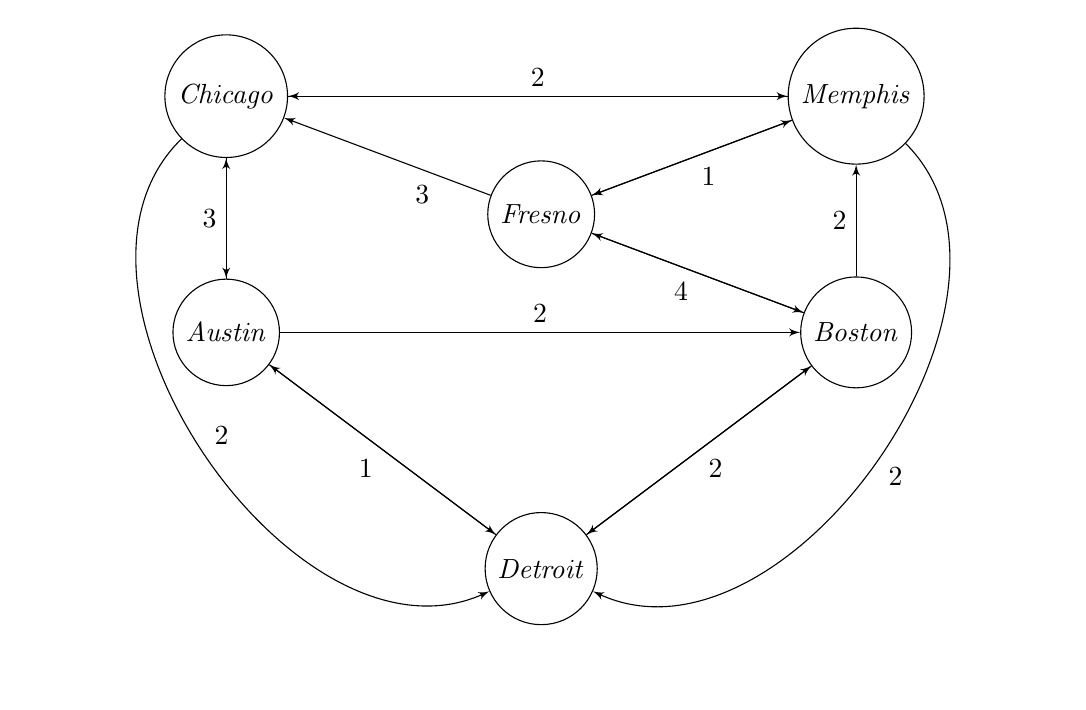
\begin{tikzpicture}
\tikzset{vertex/.style = {shape=circle,draw,minimum 
size=1.5em}}
\tikzset{edge/.style = {->,> = latex'}}
% vertices
\node[vertex] (a) at  (0,0) {$\mathit{Chicago}$};
\node[vertex] (b) at  (4,-6) {$\mathit{Detroit}$};
\node[vertex] (c) at  (8,0) {$\mathit{Memphis}$};
\node[vertex] (d) at  (8,-3) {$\mathit{Boston}$};
\node[vertex] (a1) at (0,-3) {$\mathit{Austin}$};
\node[vertex] (a2) at (4,-1.5) {$\mathit{Fresno}$};
%edges
\draw[edge] (a) to [bend right=80pt] node [auto] {2} (b);
\draw[edge] (a) to (a1);
\draw[edge] (a) to node [auto] {2} (c);
\draw[edge] (b) to (d);
\draw[edge] (b) to node [auto] {1} (a1);
\draw[edge] (c) to (a);
\draw[edge] (c) to node [auto] {1} (a2);
\draw[edge] (c) to [bend left=80pt] node [auto] {2}(b);
\draw[edge] (d) to node [auto] {2} (c);
\draw[edge] (d) to node [auto] {4} (a2);
\draw[edge] (d) to node [auto] {2} (b);
\draw[edge] (a1) to node [auto] {3} (a);
\draw[edge] (a1) to node [auto] {2} (d);
\draw[edge] (a1) to (b);
\draw[edge] (a2) to node [auto,near start] {3} (a);
\draw[edge] (a2) to (c);
\draw[edge] (a2) to (d);
\end{tikzpicture}
\end{center}
\caption{Graph of the cities}
\end{figure}
The \hex{}-program for the Travelling salesperson problem is 
encoded as follows:
\begin{exmp}
\label{travellingsalesperson}
\begin{align*}
\rowprefix{r_1} & startingCity(austin).\\
\rowprefix{r_2} & budgetB(11).\\
\\
\rowprefix{r_3} & \mathit{cityOfDegree(P,0,P,0)} \leftimpl 
\mathit{startingCity(P).} \\
& \\
\rowprefix{r_4} & \mathit{cityOfDegree(F1, DegPlus, F2, Cost)} 
\leftimpl \mathit{cityOfDegree(\_, Deg, F1, \_)}, \\ 
&\ext{edges}{F1}{F2, Cost}, \mathit{DegPlus=DegPlus+1}, 
DegPlus < 4, \\ & \#int(DegPlus), \#int(Deg)), \#int(Cost). 
\\
\rowprefix{r_5}& \mathit{node(Y)} \leftimpl 
\mathit{cityOfDgree(X, V, Y, C)}.\\
\rowprefix{r_6}& \mathit{edge}(X, Y) \leftimpl 
\mathit{cityOfDegree(X, V, Y, C).} \\
\rowprefix{r_7} & cost(X,Y,C) \leftimpl cityOfDegree(X, V, Y, C). 
\end{align*}
\begin{align*}
\rowprefix{r_8} & \{ cycle(X,Y) : edge(X,Y) \} = 1 \leftimpl 
node(X). \\
\rowprefix{r_9} &  \{ cycle(X,Y) : edge(X,Y) \} = 1 \leftimpl 
node(Y). \\
& \\
\rowprefix{r_{10}} & costCalculated(X) \leftimpl \#sum \{C,X,Y : 
cycle(X,Y), cost(X,Y,C)\} = X \\
\rowprefix{r_{11}} & withinBudget(B,C) \leftimpl budget(B), 
costCalculated(C), B \geeq C. \\
\rowprefix{r_{12}} & \leftimpl  budgetB(B), costCalculated(C), 
\nott \thinspace \mathit{withinBudget(B,C).} \\
& \\
\rowprefix{r_{13}} & reached(Y) \leftimpl cycle(C, Y), startingCity(C). \\
\rowprefix{r_{14}} & reached(Y) \leftimpl cycle(X,Y), 
reached(X). \\
\rowprefix{r_{15}} & \leftimpl node(Y), \nott \thinspace 
\mathit{reached(Y)}. \\
& \\
\rowprefix{r_{16}} & :\sim cycle(X,Y), cost(X,Y,C). [C:1] 
\end{align*}
\end{exmp}
In rule $\row{r_1}$ we have a fact which specifies the starting 
city. 
It is important to notice that in our program the starting 
point for the travelling salesperson may change and it is not 
fixed. The salesperson should start his trip from the 
city specified by the fact from $\row{r_1}$ and also finish 
his trip there if there is such a cycle which covers all 
other cities in the graph. Rule $\row{r_2}$ is a fact which defines the 
available budget of the salesperson. An atom $\mathit{cityOfDegree(R,D,S,C)}$ keeps 
track of the cities newly discovered defined as successor 
nodes $S$ for the root node $R$, their distances from the 
root node as $D$ and the weight of the edge between $R$ and $S$ 
denoted as $C$. Rule $\row{r_3}$ defines the starting city for 
the path candidate. Rule $\row{r_4}$ is responsible for 
generating a graph of 
the cities discovered. It is using the external atom 
$\mathit{\&edges}$ to load new cities from the external 
file and use them in the program. An external atom is of 
the form $\ext{edges}{F1}{F2,Cost}$ where $\mathit{F1}$ 
represents the predecessor node for which we are finding 
all successor 
nodes. $\mathit{F2}$ returns all successor nodes of 
$\mathit{F1}$ and $\mathit{Cost}$ is an integer value which 
represents weight of the edge between $\mathit{F1}$ and 
$\mathit{F2}$. $\mathit{DegPlus}$ is here set to be 4, which means we can go at most three edges far from the root node. 
There are many advantages of using an external atom of this
type:
\begin{itemize}
\item The graph may be very large and it is not possible to load it 
at once as a set of edges specified manually.
\item We do not know the graph completely (e.g., due to limited capabilities of a web service).
\item We want to analyze only a subgraph of the graph that is 
reachable from the node specified.
\end{itemize}    
In $\row{r_5}$, $\row{r_6}$ and $\row{r_7}$ the program is extracting 
$\mathit{nodes}, \mathit{edges}$ and $\mathit{costs}$ of 
the edges from the $\mathit{cityOfDegree}$ atoms. 

The rules $\row{r_8}$ and $\row{r_9}$ assert that every 
node must have exactly one outgoing and exactly one 
incoming edge, respectively, belonging to the cycle. The meaning of the two rules is described before in Section 
\ref{conditions}.

In $\row{r_{10}}$ we use aggregates (cf. Section 
\ref{aggregates}) to find the sum $X$ of the costs over the 
$\mathit{cycle(X,Y)}$. In rule $\row{r_{11}}$, an atom 
$\mathit{withinBudget(B,C)}$ is true if the term of the 
$\mathit{costCalculated(C)}$ is less than or equal to the 
term of $\mathit{budgetB(B)}$ available. The integrity 
constraint $\row{r_{12}}$ ensures that in the answer 
set overall sum of the costs for the cycle will be less 
than or equal to the budget available. The same rules can be applied to limit length travelled or time spent.

Rules $\row{\row{r_{13}}}$ and $\row{r_{14}}$ check whether all 
nodes 
are reached by a cycle candidate produced by the rules 
$\row{r_8}$ and $\row{r_9}$.  Note that rule $\row{r_8}$ builds on the
assumption that the cycle starts at city Austin. The second 
rule in $\row{r_9}$ states that, from a reached node $X$, an 
adjacent node $Y$ can be reached via a further edge in the 
cycle. It makes sure that all nodes will be reached with the 
cycle given \cite{gkklorst2015}. The integrity constraint $\row{r_{15}}$ 
eliminates answer sets where not all nodes in the graph are reached.

In order to minimize costs, we add the following 
optimization statement: \\
\centerline{$:\sim cycle(X,Y), cost(X,Y,C). \  [C:1].$}
Here, edges belonging to the cycle are weighted according 
to their costs and \dlvhex{} lists optimal answer sets only.

\subsubsection{Problem Solution}
For this example optimal answer set 
is as follows:
\begin{align*}
\{&  cycle(austin,boston), 
cycle(boston,memphis),cycle(detroit,austin), \\
& cycle(chicago,detroit), 
cycle(memphis,fresno),cycle(fresno,chicago) \} \\
& <[11:1]>.
\end{align*}
Note that we omitted input facts and intermediate results from the answer and show only the atoms specifying the final tour (optimal) to make 
answer set easier to read. The route which satisfies all given constraints is: Austin $\rightarrow$ Boston $\rightarrow$ Memphis $\rightarrow$ Fresno $\rightarrow$ Chicago $\rightarrow$ Detroit $\rightarrow$ Austin with the minimum cost of 11. 




\subsection{Example 3}
\label{example3}
The last example is from the group of pathfinding problems and it considers pathfinding for multiple agents.
 
\subsubsection{Problem Instance}
Pathfinding for a single agent is the problem of planning a 
route from an initial
location to a goal location in an environment, going around 
obstacles. 
Pathfinding for multiple agents also aims to plan such 
routes for each agent, 
subject to different constraints, such as restrictions on 
the length of each path 
or on the total length of paths, no self-intersecting 
paths, no intersection of 
paths/plans, no crossing/meeting each other.  It also has 
variations for finding optimal solutions, e.g., with 
respect 
to the maximum path length, or the sum of plan lengths. 
These problems are important
for many real-life applications, such as motion planning, 
vehicle routing, environmental monitoring, patrolling, 
computer games \cite{ekos2013}. We consider the 
problem 
where multiple agents need to find paths 
from their respective starting locations to their goal 
locations, ensuring that 
paths do not collide with static obstacles and that no two 
agents collide with 
each other. 

\subsubsection{Problem Encoding}
The \hex-program for the problem introduced in the previous 
subsection is as follows:
\begin{exmp}
\label{pathfindingAgent}
\begin{align*}
\rowprefix{r_1} & startingNode(one). \\
\rowprefix{r_2} & nodeOfDegree(P,0,P) \leftimpl startingNode(P). 
\\
\rowprefix{r_3} & nodeOfDegree(F1, DegPlus, F2) \leftimpl 
nodeOfDegree(\_, Deg, F1), \\ & \ext{edges}{F1}{F2}, 
DegPlus=Deg+1, DgPlus <= 5, \#int(DegPlus), \\ &\#int(Deg). 
\\
\rowprefix{r_4} & node(Y) \leftimpl nodeOfDegre(X, V, Y).  \\
\rowprefix{r_5} & edge(X,Y) \leftimpl nodeOfDegree(X,V,Y).\\
\\
\rowprefix{r_6} &  \mathit{agent(1). } \ \mathit{ agent(2). }\\
\rowprefix{r_7} & \mathit{start(1,one).} \ \mathit{ 
start(2,four).} \\
\rowprefix{r_8} & \mathit{goal(1,ten).} \ \mathit{ 
goal(2,eleven).} \\
\\
\rowprefix{r_9} & clear(V) \leftimpl \mathit{node(V)}, V \neq 
\mathit{three}\\ 
\\
\rowprefix{r_{10}} & guessPath(I,0,V) \leftimpl start(I,V). \\
\rowprefix{r_{11}} &  \mathit{guessPath(I, TPlus, U)} \vee 
\mathit{nguessPath(I, TPlus, U)} \leftimpl 
\mathit{agent(I)}, \\ &  \mathit{guessPath(I, T, V)},  
\mathit{edge(U,V)}, \mathit{TPlus=T+1}, 
\mathit{\#int(TPlus)}, \mathit{\#int(T).}  \\
\rowprefix{r_{12}} &  \leftimpl 1 \neq \mathit{\#count\{ U 
\colon guessPath(I, T, U) \}}, \mathit{agent(I)}, 
\mathit{\#int(T)}.  \\
\\
\row{\row{r_{13}}} \colon &  visit(I, V) \leftimpl guessPath(I,T,V). \\
\\
\rowprefix{r_{14}} & \leftimpl goal(I, V), \nott \thinspace  
\mathit{visit(I, V).} \\
\rowprefix{r_{15}} &  \leftimpl guessPath(I, T, V), 
path(I^{\prime},T,V), X \lesseq XP. \\
\rowprefix{r_{16}} &  \leftimpl guessPath(I,T,V), \nott \thinspace  
\mathit{clear(V).}\\
\\
\rowprefix{r_{17}} &  \mathit{path(I,V,U,T,ValidOrNot)} 
\leftimpl \mathit{agent(I)}, \\ & \mathit{guessPath(I, T, 
V)}, \mathit{guessPath(I, TPlus, U)}, \\ & \ext{check}{U, 
V, T, I}{ValidOrNot}, \mathit{TPlus=T+1}, \#int(T), 
\#int(TPlus).  \\
\rowprefix{r_{18}} & \leftimpl path(I, V, U, T, invalid). 
\end{align*}
\end{exmp}


In the first part of the program we load the graph using 
the $\&edges$ external atom. This atom cyclically discovers 
nodes and edges from the external file. In $\row{r_4}$ we 
extract node $Y$ whenever an atom $\mathit{nodeOfDegree(X, 
V, Y)}$ is true. Similar as in the previous rule $\row{r_5}$ extracts an edge from $X$ to $Y$ if an atom 
$\mathit{nodeOfDegree(X, V,Y)}$ is true. 

From $\row{r_6}$ to $\row{r_8}$ we define a set of facts. 
The facts $\row{r_6}$ represent different agents in the program. 
Facts $\row{r_7}$ and $\row{r_8}$ define initial and 
destination nodes for the agents.  

Rule $\row{r_9}$ 
represents that vertex $V$ is free and does not have any 
obstacle on it. Rules $\row{r_{10}}$, $\row{r_{11}}$ and 
$\row{r_{12}}$ guesses the next node to be visited by the agent, from 
node $U$ to the node $V$. The agent can either visit a new node 
using an existing edge or stay at the same node and wait. 
In rule $\row{r_{10}}$, the initial location for the path is set. Rule $\row{r_{11}}$ 
with a disjunctive head (cf. Section~\ref{disjunction}) decides either to include the outgoing edge 
from the node $U$ to the path or to omit it from the path. 
This step is cyclically performed until the goal nodes are not 
reached. The constraint $\row{r_{12}}$ eliminates all answer sets in which there is more than one outgoing edge 
selected at some time point from node $U$. Thus, for each step 
the agent has to select a single edge since it cannot be at the 
two different locations at the same time. Rule $\row{\row{r_{13}}}$ computes which nodes are visited using the path 
guessed. The integrity constraint $\row{r_{14}}$ ensures that 
each agent reaches its destination node. We ensure that 
agents do not collide with each other using constraint 
$\row{r_{15}}$. We also ensure that agents do not go through 
obstacles using constraint $\row{r_{16}}$. 

We represent path plans by atoms of the form 
$\mathit{path(I, V, U, T, ValidOrNot)}$ which specify that 
at time step $T$, agent $I$ moves from a node $V$ to a 
node $U$. An external atom is used to decide whether that move is valid or invalid. The last 
two rules $\row{r_{17}}$ and $\row{r_{18}}$ check if the overall path is valid or invalid. Agents can only know what are the edges 
available in the graph and make the guess in which 
direction they should go. Consider that an agent selects 
some 
edge but it becomes unusable because of some reasons in the meantime. 
The reasons may be obstacles in the environment, too narrow corners, too small doors or any change on 
the graph or on the environment which is not considered as 
a fact in the program. By introducing this property we have a dynamic problem. To perform this check we 
can use only an external source. The external source is of the 
form \ext{check}{U,V,T,I}{ValidOrNot} and checks is the 
guessed move of the agent $I$ from $U$ to $V$ at time $T$ is 
$\mathit{valid}$ or $\mathit{invalid}$. In the case that 
any of the moves in the guessed path is invalid, the whole 
answer set is eliminated. If no invalid moves are guessed in the path, it means that solution is the answer set of the program.            

\subsubsection{Problem Solution} 
Let us solve the problem using the following graph.  
\begin{figure}
\begin{center}
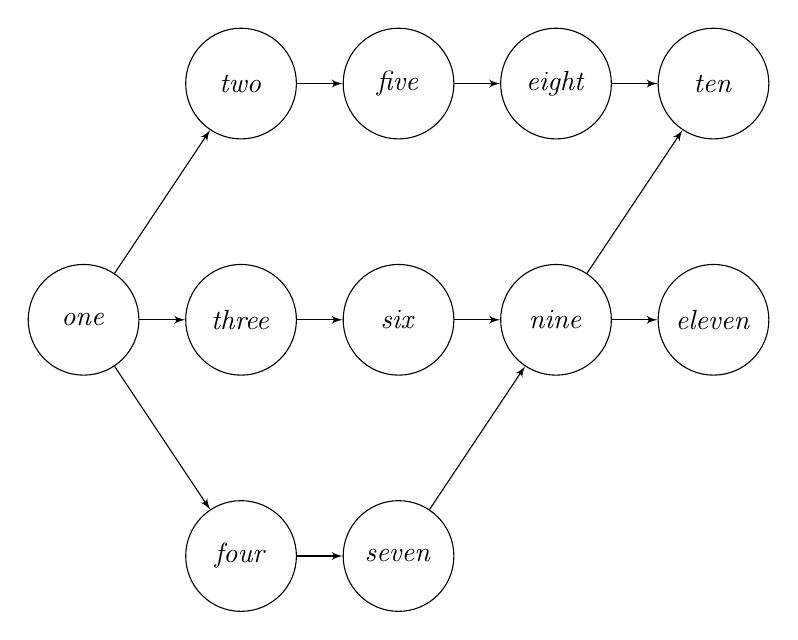
\begin{tikzpicture}
\tikzset{vertex/.style = {shape=circle,draw,minimum 
size=4em}}
\tikzset{edge/.style = {->,> = latex'}}
% vertices
\node[vertex] (a) at  (0,3) {$\mathit{one}$};
\node[vertex] (b) at  (2,6) {$\mathit{two}$};
\node[vertex] (c) at  (2,3) {$\mathit{three}$};
\node[vertex] (d) at  (2,0) {$\mathit{four}$};
\node[vertex] (e) at  (4,6) {$\mathit{five}$};
\node[vertex] (f) at  (4,3) {$\mathit{six}$};
\node[vertex] (g) at  (4,0) {$\mathit{seven}$};
\node[vertex] (i) at  (6,6) {$\mathit{eight}$};
\node[vertex] (j) at  (6,3) {$\mathit{nine}$};
\node[vertex] (k) at  (8,6) {$\mathit{ten}$};
\node[vertex] (l) at  (8,3) {$\mathit{eleven}$};
%edges
\draw[edge] (a) to (b);
\draw[edge] (a) to (c);
\draw[edge] (a) to (d);
\draw[edge] (b) to (e);
\draw[edge] (c) to (f);
\draw[edge] (d) to (g);
\draw[edge] (e) to (i);
\draw[edge] (f) to (j);
\draw[edge] (g) to (j);
\draw[edge] (i) to (k);
\draw[edge] (j) to (l);
\draw[edge] (j) to (k);
\end{tikzpicture}
\end{center}
\caption{Simulation of the environment used by agents}
\end{figure}
The graph is again loaded from the external file and not 
specified as a set of facts. We know that there is an obstacle at node $\mathit{three}$, so any answer set with node 
$\mathit{three}$ in the path is removed. All other 
constraints must be satisfied as well. Note that we have 
omitted most of the atoms in order to emphasize the actual 
solution (in order to see how to filter out answer sets and 
show only specific atoms at the output refer to the 
Section~\ref{sec:commandline}; in our answer set, we are 
interested only in $\mathit{path}$ atoms since we want to 
see what is the path from the initial node $U$ to the 
destination node $V$). One answer set is as follows:
\\Answer Set 1:
\begin{align*}
\{ & path(1,one,two,0,valid), path(1,two,five,1,valid),
\\ & path(1,five,five,2,valid), path(2,four,four,0,valid),
\\ & path(2,four,seven,1,valid), 
path(1,five,eight,3,valid),
\\ & path(2,seven,nine,2,valid), path(1,eight,ten,4,valid),
\\ & 
path(2,nine,eleven,3,valid),path(2,eleven,eleven,4,valid) 
\}
\end{align*} 
Here, $\mathit{agent(1)}$ follows the path:
one $\rightarrow$ two $\rightarrow$ five $\rightarrow$ five 
$\rightarrow$ eight $\rightarrow$ ten. At each time 
point an agent chooses either to wait or to move to 
the another node. At $t=2$ the $\mathit{agent(1)}$ chooses 
to wait and not to move. The same logic is applied for the 
$\mathit{agent(2)}$. To show different possible choices we are 
giving two answer sets more:
\\Answer Set 2:
\begin{align*}
\{ & path(1,one,two,0,valid),path(1,two,five,1,valid),
\\ & path(1,five,five,2,valid),path(2,four,seven,0,valid),
\\ & path(1,five,eight,3,valid),path(2,seven,nine,1,valid),
\\ & path(2,nine,nine,2,valid),path(1,eight,ten,4,valid),
\\ & 
path(2,nine,eleven,3,valid),path(2,eleven,eleven,4,valid)\}
\end{align*}
In the second answer set, the path for the first agent did not 
change. However, the second agent changes its path and instead 
of waiting at $t=0$ at node four it moves to the node 
seven.  
\\Answer Set 3:
\begin{align*}
\{ & path(1,one,four,0,valid), path(1,four,seven,1,valid),
\\ & path(1,seven,nine,2,valid), path(2,four,seven,0,valid),
\\ & path(2,seven,nine,1,valid), 
path(1,nine,ten,3,valid),
\\ & path(2,nine,eleven,2,valid), path(1,ten,ten,4,valid),
\\ & 
path(2,eleven,eleven,3,valid),path(2,eleven,eleven,4,valid) 
\}
\end{align*} 

\section{External Interfaces}
\label{sec:externalInterfaces}
This section discusses the implementation of external sources. One important design principle was to provide a 
mechanism to easily add further external atoms, as introduced in Section~\ref{extatoms}, without 
having to recompile the main application.
 
Formally, an external atom is defined to evaluate to true
or false, depending on a number of parameters:
\begin{itemize}
\item An interpretation (a set of atoms)
\item A list of input constants
\item A list of output constants
\end{itemize}  
However, it is more intuitive and convenient to think of an 
external atom not as being boolean, but rather functional:
depending on a given interpretation and a list of input 
constants, it returns output tuples for which it is true. For instance, the 
external atom to import triples from RDF files has the 
form: \\
\centerline{$\ext{rdf}{uri}{X,Y,Y}$} 
where $\mathit{uri}$ stands for a string denoting the RDF-source and X,Y, and Z are variables that represent an RDF-triples from the specified source.

\subsection{Information Flow}
The interface that is used by \dlvhex{} to access a plugin 
follows very closely this semantics. For each atom, a 
retrieval function has to be implemented, which receives a 
query object and has to return an answer-object. The 
query object carries the input interpretation as well as 
the ground input parameters of the external atom call, 
while the answer object is a container for the output 
tuples of the external atom's function.   

\subsection{Types of Input Parameters}
In practice, only 
parts of the interpretation might be needed. Considering 
this as well as for efficiency reasons, there are three types of input parameters: 
\begin{itemize}
\item Constant parameters
\item Predicate parameters
\item Tuples
\end{itemize}

A parameter of type \emph{constant} is not related to the 
interpretation at all, like in the previous example of the 
RDF-atom where we have strings as a constant input to the external atom. 

A parameter is of type \emph{predicate} means that 
all atoms in the interpretation with this predicate are 
necessary for the external atom. Let us assume, we have an external 
atom that calculates the overall price of a number of books 
given by their ISBN number:\\
\centerline{$\ext{overallbookprice}{isbn}{X}$}
The single input parameter of this atom would be of type 
\emph{predicate}, meaning that not the constant itself is 
necessary for the atom's function, but the part of the 
interpretation with this predicate. So if we have, e.g.,\\ 
I = \{$\mathit{isbn(``0}$-$\mathit{19}$-$\mathit{82183}$-$\mathit{6")}$, $ \mathit{isbn(``0}$-$\mathit{201}$-$\mathit{99954}$-$\mathit{4")}$, $p(a)$, $q(b)$ $\dots$ \}
the atom's function will be called with the filtered interpretation: \\
$I=$\{$\mathit{isbn(``0}$-$\mathit{19}$-$\mathit{82183}$-$\mathit{6")}$, $ \mathit{isbn(``0}$-$\mathit{201}$-$\mathit{99954}$-$\mathit{4")}$\}

A parameter of type \emph{tuple} represents a meta category standing for an arbitrary number of constant input parameters. This is useful when we have to send multiple constant parameters separately, e.g., for \\
\centerline{$\ext{concat}{string1, string2, string3, \dots}{Out}$}. 

Specifying the type of input parameters not only helps to 
single out the relevant part of the interpretation, but 
also supports \dlvhex{} in calculating the dependencies 
within a \hex-program. Plugins can be implemented either in Python or C++, as shown in the following two subsections.

\subsection{Python}
With \dlvhex{} version 2.4.0, a Python plugin interface was 
introduced, which supports Python scripts that provide 
functions to realise custom external atoms. For every Python plugin two tasks are to be carried out:
\begin{itemize}
\item Write a new Python script which contains a register function and imports the package \dlvhex{}.
\item Write another function for each external atom, and export this function using the $\mathit{register}$ function. 
\end{itemize}
The \verb+register+ function has the following form:
\begin{verbatim} 
def register():
  dlvhex.addAtom("Atom_Name",(Input_Parameters),Output_Arity) 
\end{verbatim}
It contains a call of \verb+addAtom+ for each external atom. Each call specifies a tuple of arity 3:
\begin{itemize}
\item \verb+Atom_Name+ is the name of the 
external predicate.
\item \verb+Input_Parameters+ is a tuple of arbitrary many input parameter types. Each input parameter type is one of the 
following: \verb+dlvhex.CONSTANT+, \verb+dlvhex.PREDICATE+ or 
\verb+dlvhex.TUPLE+, as it is introduced in the previous section.
\item \verb+Output_Arity+ is an integer value representing the output arity of an atom.  
\end{itemize}
Consider the $\mathit{\&concat}$ external atom which we introduced in the previous section. It takes two strings as input and outputs their concatenation. The register function then would be as follows:
\begin{verbatim}
def register():
  dlvhex.addAtom("concat", (dlvhex.CONSTANT, dlvhex.CONSTANT), 1)  
\end{verbatim}
Once the external atom is registered successfully, it has 
to be implemented in the form of another Python function 
with an appropriate number of input parameters. It has the 
following form:  
\begin{verbatim}
def Atom_Name(Input_Parameter_1, Input_Parameter_2, ...)
  dlvhex.output((Output_Parameter_1, ...))
\end{verbatim}

The implementation of the \verb+concat+ function is as follows:
\begin{verbatim}
def concat(a,b)
  # Function body goes here
  dlvhex.output((str, ))
\end{verbatim} 
To get more familiar with Python plugins we are providing three examples as there are three possible input parameter types.

The plugin in Example~\ref{constantAsInput} uses a constant (string) input parameter. It is used in Example~\ref{faceQuery} to query all direct friends of the person of interest.
\begin{exmp}
\label{constantAsInput}
\begin{verbatim}

1:  import dlvhex
2:  import networkx as nx

3:  def friendsOf(personOfInterest):
4:    g = nx.read_weighted_edgelist("test.edgelist",nodetype=str,
                                    create_using=nx.DiGraph())
5:    friendList = g.successors(personOfInterest.value())
6:    for item in friendList:
7:      dlvhex.output((item, ))

8:  def register():
9:  prop = dlvhex.ExtSourceProperties()
10: prop.addFiniteOutputDomain(0)
11: dlvhex.addAtom("friendsOf", (dlvhex.Constant, ),1,prop)
\end{verbatim}
\end{exmp}

In the lines 1 and 2 we have imported two libraries which 
are required. We have to import the \verb+dlvhex+ 
library as for every plugin. The \verb+networkx+ library is needed in this particular example since we are 
performing graph operations (i.e. loading graphs from the file, get all successors of the node etc). 

Lines \verb+3+ to \verb+7+ implement the \verb+friendsOf+ external atom. 
It receives the name of the person as string and searches for all 
direct friends of that person in the graph, which is loaded from the file in line \verb+4+. All discovered friends, are output in line \verb+7+. 

Lines \verb+8+ to \verb+11+ register the external atom 
\verb+friendsOf+ with constant input parameter and 
single output parameter. 

The following example uses a predicate input parameter 
for the \verb+&rq+ external atom as used in Example~\ref{swimExample}. The external atom is performing 
a Web search to check the requirements for the selected location. It is of the form 
$\ext{\mathit{rq}}{\mathit{location\_choice}}
{\mathit{required\_resource}}$ which intuitively evaluates 
to true if a given location\_choice requires a certain 
required\_resource and represents such resources and their 
origin (inoutd, or loc) using predicate $\mathit{need}$. 
\begin{exmp}
\label{predicateAsInput}
\begin{verbatim}

1:  import dlvhex 

2:  def rq(location_chioce)
3:    for x in dlvhex.getTrueInputAtoms():
4:      io = {"ind":"money","amalB":"goggles","altD":"yogamat",
              "gansD":"money"}
5:      if location_chioce == x.tuple()[0]:
6:        inp = x.tuple()[1].value()
7:          if inp in io:
8:            dlvhex.output((io[inp], ))

9:  def register():
10:   dlvhex.addAtom("rq", (dlvhex.PRDICATE), ), 1)
\end{verbatim}
\end{exmp}

From line \verb+2+ to line \verb+8+ we implement the \verb+rq+ function. Line \verb+5+ filters the atoms according to the given predicate. In Line 6 we check if the predicate of the current input atom is equivalent to \texttt{location\_choice}, which specifies the selected location. Line \verb+8+ is returning  
the requirements (if any) of the location specified by variable 
\verb+inp+. Lines \verb+9+ to \verb+10+ define the register 
function for the \verb+rq+ external atom.

As mentioned above, there exists a third parameter type \emph{tuple}. It stands for an arbitrary number of constant input parameters. The following example presents the usage of a tuple in a plugin used to implement string concatenation for arbitrary many strings.  
\begin{exmp}
\label{tupleAsInput}
\begin{verbatim}

1:  import dlvhex

2:  def concat(tup):
3:    ret=" "
4:    for x in tup:
5:      ret = ret + x.value()
6:    dlvhex.output((ret, ))

7:  def register():
8:    dlvhex.addAtom("concat", (dlvhex.TUPLE, ), 1)
\end{verbatim}
\end{exmp}
This plugin receives a tuple of strings, concatenates 
them and outputs them as a single string value. The function \verb+concat+ is implemented from line \verb+2+ to \verb+6+. In line \verb+3+, an 
empty string is initialized. Inside the for loop, the input 
strings are appended to the string initialized. This process 
is continued until all strings from the tuple have been processed.  
 
A more detailed description of all methods available for the \dlvhex{} Python module can be found at:\\ \url{http://www.kr.tuwien.ac.at/research/systems/dlvhex/doc2x/}\\
\url{group__pythonpluginframework.html}
\subsection{C++}
TODO

\section{Command Line options}
\label{sec:commandline}
In this section, we briefly describe the meaning of the command line options supported by \dlvhex{}. 
Calling only \dlvhex{} without any arguments will show all 
command line options available. For each option, we indicate whether it requires an argument, and if so, we also describe its meaning. An abstract invocation of \dlvhex{} looks as follows:\\
\texttt{dlvhex2 [OPTION] FILENAME [FILENAME ...]} or \texttt{dlvhex2 [OPTION] --}

\bigskip
The following set of commands is related with Input, Output and  Reasoning options and they directly affect the result.
% Sets column space
%\def\arraystretch{2}\tabrowsep=50pt
% Sets row space
\renewcommand{\arraystretch}{1.6}
\begin{longtable}{p{2.2cm}  p{2.5cm} p{0.6cm} p{6.3cm}  } 
 & \texttt{--}& & Parse from standard input. \\ 
\texttt{-s} & \texttt{--silent}&& Do not display anything than the actual result \\ 
\texttt{-f} & \texttt{--filter=foo[,bar[,...]]} && \\
& & & Only display instances of the specified predicate(s).\\
& \texttt{--nofacts} && Do not output EDB facts. EDB facts are the facts of the program.  \\
\texttt{-n} & \texttt{--number=<num>} && Limit number of displayed models to $\langle$\texttt{num}$\rangle$, Default value is 0, which means to display all models.\\ 
\texttt{-N} & \texttt{--maxint=<num>} && Set maximum integer (\# \texttt{maxint} in the program takes precedence). \\
 & \texttt{--weaksafety} && Skip strong safety check.\\
 & \texttt{--strongsafety} && Applies traditional strong safety criteria. \\
  & \texttt{--liberalsafety} && Uses more liberal safety condition than strong safety. \\
  &\texttt{--mlp}&& Use \dlvhex{}$+$mlp solver (modular nonmonotonic logic programs).\\
  & \texttt{--forget} && Forget previous instantiations that are not involved in current computation (mlp setting). \\
  & \texttt{--split} &&Use instantiation splitting techniques.\\
  & \texttt{--noeval} && Parse the program, but do not evaluate it (only useful with \texttt{--verbose}). \\
  & \texttt{--keepnsprefix} && Keep specified namespace-prefixes in the result. \\
  & \texttt{--keepauxpreds} && Keep auxiliary predicates in answer sets. \\
\end{longtable}
\bigskip
\subsection{Plugin Options}
\begin{center}
\begin{tabular}{p{2.2cm}  p{2.5cm} p{0.6cm} p{6.3cm}  } 
 \texttt{-p}&\texttt{--plugindir=DIR}&&Specify additional directory where to look for plugin libraries (additionally to the installation plugin-dir and \texttt{\$HOME/.dlvhex/plugins}). Start with \texttt{!} to reset the preset plugin paths, e.g., ``\texttt{!:/lib}'' will use only \texttt{/lib/}.
 \\
\end{tabular}
\end{center}

\subsection{Performance Tuning Options}
\begin{center}
\begin{longtable}{p{0.7cm}  p{2.2cm} p{0.3cm} p{6.3cm}  } 
%--EXTLEARN
\multicolumn{4}{p{6cm}}{\texttt{--extlearn[=none,iobehavior,monotonicity,functionality,}} \\[-1.5ex]
\multicolumn{4}{p{6cm}}{\texttt{\hphantom{--extlearn[}linearity,neg,user,generalize]}} \\

& & & Learn nogoods from external atom evaluation (only useful with \texttt{--solver=genuineii} or \texttt{--solver=genuinegi)}.\\
&\texttt{none}:& & Deactivate external learning. \\
&\texttt{iobehaviour}:& &Apply generic rules to learn input-output behaviour. \\
&\texttt{monotonicity}:& &Apply special rules for monotonic and antimonotonic external atoms.\\
&\texttt{functionality}:& &Apply special rules for external atoms which are linear in all predicate parameters.\\
&\texttt{linearity}:& &Apply special rules for external atoms which are linear in all predicate parameters.\\
&\texttt{neg}:& &Learn negative information\\
&\texttt{user}:& &Apply user-defined rules for nogood learning\\
&\texttt{generalize}:& &Generalize learned ground nogoods to ground nogoods.\\
& & & By default all options above except ``\texttt{generalize}'' are enabled.\\
%%%%%%%%%%%%%%%%%%%
\multicolumn{4}{l}{\texttt{--supportsets}}\\
& & &Exploits support sets for evaluation.\\
%%%%%%%%%%%%%%%%%%%
\multicolumn{4}{l}{\texttt{--evalall}}\\
& & &Evaluate all external atoms in every compatibility check, even if previous external atoms already failed.  This makes nogood learning more independent of the sequence of external atom checks. Only useful with \texttt{--extlearn}.\\
%%%%%%%%%%%%%%%%%%%
\multicolumn{4}{l}{\texttt{--nongroundnogoods}}\\
& & &Automatically instantiate learned nonground nogoods.\\
%%%%%%%%%%%%%%%%%%%
\multicolumn{4}{l}{\texttt{--flpcheck=[explicit,ufs,ufsm,aufs,aufsm,none]}}\\
& & &Sets the strategy used to check if a candidate is a subset-minimal model of the reduct.\\
&\texttt{explicit}:&&Compute the reduct and compare its models with the candidate\\
&\texttt{ufs}:&&Use unfounded sets for minimality checking
\\
&\texttt{ufsm}:&&Use unfounded sets for minimality checking, do not decompose the program for UFS checking.\\
&\texttt{aufs (default)}:&&Use unfounded sets for minimality checking by exploiting assumptions\\
&\texttt{aufs}:&&Use unfounded sets for minimality checking by exploiting assumptions. Do not decompose the program for UFS checking.\\
&\texttt{none}:&&Disable the check.\\
%%%%%%%%%%%%%%%%%%%
\multicolumn{4}{l}{\texttt{--flpcriterion=[all,head,e,none]}}\\
& & & Defines the kind of cycles whose absence is exploited for skipping minimality checks.\\
&\texttt{all (default)}:&&Exploit head- and e-cycles for skipping minimality checks\\
&\texttt{head}:&& Exploit head-cycles for skipping minimality checks\\
&\texttt{e}:&&Exploit e-cycles for skipping minimality checks\\
&\texttt{none}:&& Do not exploit head- or e-cycles for skipping minimality checks\\
%%%%%%%%%%%%%%%%%%%
\multicolumn{4}{l}{\texttt{--noflpcriterion}}\\
& & & Do no apply decision criterion to skip the FLP check. (equivalent to \texttt{--flpcriterion=none)}\\
\multicolumn{4}{l}{\texttt{--ufslearn=[none,reduct,ufs]}}\\
& & & Enable learning from UFS checks (only useful with \texttt{--flpcheck=[a]ufs[m]}).\\
&\texttt{none}:&&No learning\\
&\texttt{reduct}:&&Learning is based on the FLP-reduct\\
&\texttt{ufs (default)}:&&Learning is based on the unfounded set\\
%%%%%%%%%%%%%%%%%%%
\multicolumn{4}{l}{\texttt{--eaevalheuristics=[always,periodic,inputcomplete,}}\\
\multicolumn{4}{l}{\texttt{eacomplete,post,never}}\\
& & & Selects the heuristic for external atom evaluation.\\
&\texttt{always}:&&Evaluate whenever possible\\
&\texttt{periodic}:&&Evaluate in regular intervals.\\
&\texttt{incomplete}:&&Evaluate whenever the input to the external atom is complete\\
&\texttt{eacomplete}:&& Evaluate whenever all atoms relevant for the external atom are assigned\\
&\texttt{post (default)}:&&Only evaluate at the end\\
&\texttt{never}:&&Only evaluate at the end and also ignore custom heuristics provided by plugins\\
&&&Except for heuristics "never", custom heuristics provided by external atoms overrule the global heuristics for the particular external atom.\\
%%%%%%%%%%%%%%%%%%%
\multicolumn{4}{l}{\texttt{--ufscheckheuristic=[post,max,periodic]}}\\
& & & Specifies the frequency of unfounded set checks (only useful with \texttt{--flpcheck=[a]ufs[m])}.\\
&\texttt{post (default)}:&&Do UFS check only over complete interpretations\\
&\texttt{max}:&&Do UFS check as frequent as possible and over maximal subprograms\\
&\texttt{periodic}:&&Do UFS check in periodic intervals\\
%%%%%%%%%%%%%%%%%%%
\multicolumn{4}{l}{\texttt{--modelqueuesize=N}}\\
& & & Size of the model queue, i.e. number of models which can be computed in parallel. Default value is 5. The option is only useful for clasp solver.\\
%%%%%%%%%%%%%%%%%%%
\multicolumn{4}{l}{\texttt{--solver=S}}\\
& & & Use S as ASP engine, where S is one of \dlv{}, \dlvdb{}, \libdlv{}, \libclingo{}, \genuineii{}, \genuinegi{}, \genuineic{}, \genuinegc{} (\texttt{genuineii}=(i)nternal grounder and (i)nternal solver; \texttt{genuinegi}=(g)ringo grounder and (i)nternal solver \texttt{genuineic}=(i)nternal grounder and (c)lasp solver; \texttt{genuinegc}=(g)ringo grounder and (c)lasp solver).\\
%%%%%%%%%%%%%%%%%%%
\multicolumn{4}{l}{\texttt{--claspconfig=C}}\\
& & & If clasp is used, configure it with \texttt{C} where \texttt{C} is parsed by clasp config parser, or \texttt{C} is one of the predefined strings frumpy, jumpy, handy, crafty, or trendy.\\
%%%%%%%%%%%%%%%%%%%
\texttt{-e}& \multicolumn{3}{l}{\texttt{--heuristics=H}}\\
& & & Use \texttt{H} as evaluation heuristics, where \texttt{H} is one of\\
&\texttt{old}:&&Old dlvhex behavior\\
&\texttt{trivial}:&&Use component graph as eval graph (much overhead)\\
&\texttt{easy}:&&Simple heuristics, used for LPNMR2011\\
&\texttt{greedy (default)}:&& Heuristics with advantages for external behaviour learning\\
&\texttt{monolithic}:&& Put entire program into one unit\\
&\texttt{manual:<file>:} &&  Read ``collapse'' $\langle$ idxs $\rangle$ share $\langle$idxs$\rangle$ commands from $\langle$file$\rangle$ where component indices $\langle$idx$\rangle$ are from \texttt{--graphviz=comp}\\
&\texttt{asp:<script>}:&&Use asp program $\langle$\texttt{script}$\rangle$ as eval heuristic\\
%%%%%%%%%%%%%%%%%%%
\multicolumn{4}{l}{\texttt{--forcegc}}\\
& & & Always use the guess and check model generator.\\
%%%%%%%%%%%%%%%%%%%
\texttt{-m}& \multicolumn{3}{l}{\texttt{--modelbuilder=M}}\\
& & & Use \texttt{M} as model builder, where \texttt{M} is one of (online,offline).\\
%%%%%%%%%%%%%%%%%%%
\multicolumn{4}{l}{\texttt{--nocache}}\\
& & &Do not cache queries to and answers from external atoms.\\
%%%%%%%%%%%%%%%%%%%
\multicolumn{4}{l}{\texttt{--iauxinaux}}\\
& & &Keep auxiliary input predicates in auxiliary external atom predicates (can increase or decrease efficiency).\\
%%%%%%%%%%%%%%%%%%%
\multicolumn{4}{l}{\texttt{--constspace}}\\
& & &Free partial models immediately after using them. This may cause some models to be computed multiple times. (Not with monolithic.)\\
\end{longtable}
\end{center}
\subsection{Debugging and General Options}
\begin{center}
\begin{longtable}{p{2.2cm}  p{2.5cm} p{0.6cm} p{6.3cm}  }
%%%%%%%%%%%%%%%%%%%
\multicolumn{4}{l}{\texttt{--dumpevalplan=F}}\\
& & & Dump evaluation plan (usable as manual heuristics) to file \texttt{F}.\\
%%%%%%%%%%%%%%%%%%%
\texttt{-v}& \multicolumn{3}{l}{\texttt{--verbose[=N]}}\\
& & & Specify verbose category (if option is used without [\texttt{=N}] then default is 1):\\
&\texttt{1}:&& Program analysis informations (including dot-file)\\
&\texttt{2}:&& Program modifications by plugins\\
&\texttt{4}:&& Intermediate model generation info\\
&\texttt{8}:&& Timing information (only if configured with \texttt{\texttt{--enable-benchmark}})\\
&&&add values for multiple categories.\\
%%%%%%%%%%%%%%%%%%%
\multicolumn{4}{l}{\texttt{--dumpstats}}\\
& & & Dump certain benchmarking results and statistics in CSV format. (Only if configured with --enable-benchmark.)\\
%%%%%%%%%%%%%%%%%%%
\multicolumn{4}{l}{\texttt{--graphviz=G}}\\
& & & Specify comma separated list of graph types to export as .dot files. Default is none, graph types are:\\
&\texttt{dep}:&& Dependency Graph (once per program)\\
&\texttt{cycinp}:&& Graph for analysis cyclic predicate inputs (once per G\&C-eval unit)\\
&\texttt{comp}:&& Component Graph (once per program)\\
&\texttt{eval}:&& Evaluation Graph (once per program)\\
&\texttt{model}:&& Model Graph (once per program, after end of computation)\\
&\texttt{imodel}:&& Individual Model Graph (once per model)\\
&\texttt{attr}:&& Attribute dependency graph (once per program)\\
%%%%%%%%%%%%%%%%%%%
\multicolumn{4}{l}{\texttt{--version}}\\
& & & Shows version information.\\
%%%%%%%%%%%%%%%%%%%
\multicolumn{4}{l}{Plugin help for dlvhex-manualevalheuristicsplugin[internal]:}\\
\multicolumn{4}{l}{\texttt{--manualevalheuristics-enable}}\\
& & & Enable parsing and processing of ``\texttt{\#evalunit(...)}'' instructions.\\
%%%%%%%%%%%%%%%%%%%
\multicolumn{4}{l}{Plugin help for dlvhex-manualevalheuristicsplugin[internal]:}\\
\multicolumn{4}{l}{\texttt{--query-enable=[true,false]}}\\
& & & Enable or disable the querying plugin (default is disabled).\\
\multicolumn{4}{l}{\texttt{--query-brave}}\\
& & & Do brave reasoning.\\
\multicolumn{4}{l}{\texttt{--query-all}}\\
& & & Give all witnesses when doing ground reasoning.\\
\multicolumn{4}{l}{\texttt{--query-cautious}}\\
& & & Do cautious reasoning.\\
%%%%%%%%%%%%%%%%%%%
\multicolumn{4}{l}{Plugin help for dlvhex-aggregateplugin[internal]:}\\
\multicolumn{4}{l}{\texttt{--aggregate-enable[=true,false]}}\\
& & & Enable aggregate plugin (default is enabled).\\
%%%%%%%%%%%%%%%%%%%
\multicolumn{4}{l}{\texttt{--aggregate-mode=[native,ext]}}\\
& & & Enable aggregate plugin (default is enabled).\\
&\texttt{native (default)}:&& Keep aggregates (but simplify them to some basic types).\\
&\texttt{ext}:&& Rewrite aggregates to an external atoms.\\
%%%%%%%%%%%%%%%%%%%
\multicolumn{4}{l}{\texttt{--aggregate-allowaggextcycles}}\\
& & & Allows cycles which involve both aggregates and external atoms. If the option is not specified, such cycles lead to abortion; if specified, only a warning is printed but the models might be not minimal. With \texttt{--aggregate-mode=ext}, the option is irrelevant as aggregates are replaced by external atoms (models will be minimal in that case). See examples/aggextcycle1.hex..\\
%%%%%%%%%%%%%%%%%%%
\multicolumn{4}{l}{Plugin help for dlvhex-strongnegationplugin[internal]:}\\
\multicolumn{4}{l}{\texttt{--strongnegation-enable[=true,false]}}\\
& & & Enable or disable strong negation plugin (default is enabled).\\ 
%%%%%%%%%%%%%%%%%%%
\multicolumn{4}{l}{Plugin help for dlvhex-weakconstraintplugin[internal]:}\\
\multicolumn{4}{l}{\texttt{--weak-enable[=true,false]}}\\
& & & Enable or disable weak constraint plugin (default is enabled). \texttt{--weak-allmodels} Display all models also under weak constraints.\\ 
%%%%%%%%%%%%%%%%%%%
\multicolumn{4}{l}{Plugin help for dlvhex-functionplugin[internal]:}\\
\multicolumn{4}{l}{\texttt{--function-maxarity=<N>}}\\
& & & Maximum number of output terms in functionDecompose.\\ 
%%%%%%%%%%%%%%%%%%%
\multicolumn{4}{l}{\texttt{--function-rewrite}}\\
& & & Rewrite function symbols to external atoms.\\ 
%%%%%%%%%%%%%%%%%%%
\multicolumn{4}{l}{Plugin help for dlvhex-choicePlugin[internal]:}\\
\multicolumn{4}{l}{\texttt{--choice-enable[=true,false]}}\\
& & & Enable choice rules (default is enabled).\\
%%%%%%%%%%%%%%%%%%%
\multicolumn{4}{l}{Plugin help for dlvhex-conditionalLiteralPlugin[internal]:}\\
\multicolumn{4}{l}{\texttt{--conditinal-enable[=true,false]}}\\
& & & Enable conditional literals (default is enabled).\\
%%%%%%%%%%%%%%%%%%%
\multicolumn{4}{l}{Plugin help for dlvhex-pythonplugin[internal]:}\\
\multicolumn{4}{l}{\texttt{--python-plugin=[PATH]}}\\
& & & Add Python script "PATH" as new plugin.\\
\multicolumn{4}{l}{\texttt{--python-main=PATH}}\\
& & & Call method "main" in the specified Python script (with dlvhex support) instead of evaluating a program.\\
\multicolumn{4}{l}{\texttt{--python-arg=ARG}}\\
& & &Passes arguments to Python (sys.argv) (can be used multiple times).\\
\end{longtable}
\end{center}


\section{Input-related warnings and errors}
\label{sec:inputRelatedWarnings}
This section explains the most frequent errors, warnings, and info messages related
to inappropriate inputs or command line options. All messages are printed to the
standard error stream.

\subsection{Syntax Errors}
In this section we consider errors emitted during the parsing and checking of logic programs.
These errors include information to ease finding and fixing the problem. Each of the error messages below
shows a line in which the error appears, followed by the type of the error and a short description of the error in standard error stream.
\begin{align*}
 & \texttt{8 \ unparsed \  ``go $\leftimpl$ goto(X)'' }\\
 & \texttt{8 ----------$\widehat{}$} \\
 & \texttt{GeneralError:Syntax \ Error: \ Could \ not \ parse \ complete \ input!}
\end{align*}

To correct this error, please investigate the indicated location and make sure that the input respects the grammar as shown in Section~\ref{sec:inputLang} (like a missing period, an unmatched parenthesis,
etc.).

\subsection{Plugin-related errors}
In this section we explain exceptions and errors 
which may occur while working with external atoms 
or plugins in which we have implemented desired external atom functionality (e.g. Python or C++ plugin). 

The following exception occurs whenever we try to
load a plugin from a nonexisting file, either from the Python or C++ file.
\begin{align*}
\texttt{Exception: nonexisting\_file\_name.py : no such file}
\end{align*}
$\texttt{nonexisting\_file\_name.py}$ does not exist in the current directory and should be replaced with
the right file which contains implementation for the external atom(s) used in \hex{}-program.

The following error occurs if we do not provide an external atom specification and implementation 
in the source file but we use it in the \hex{}-program. The error looks as below:
\begin{align*}
& \texttt{GeneralError: Fatal: did not find plugin atom for predicate}\\ 
& \texttt{"ext\_atom"}
\end{align*}  
From the description above we can see that there is no plugin atom for the predicate \texttt{ext\_atom}
in the source file which is passed as parameter from the command line. Implementation for the predicate 
\texttt{ext\_atom} should be added to the plugin source file.

Another error occurs if the output arity of an external atom does not 
match its specification in the source file. The error is given below:
\begin{align*}
& \texttt{GeneralError: External Atom \ext{rq}{ind}{C,A} has a wrong} \\
& \texttt{output arity (should be 1)}
\end{align*}  

\subsection{Safety Checking}
\label{safetyCheck}
If any of the variables used in the \hex{}-program does not satisfy safety conditions listed below, the program is not safe and an error occurs. Examples and explanations in the following subsections are used from \cite{brfwilvpg2009}. 

\subsubsection{Regular Safety}
\dlvhex{} imposes a safety condition on variables in rules. 
This guarantees that a rule has only finitely many ground instances.

\paragraph{Standard, Arithmetic and Comparative Predicates}
A variable $X$ in an aggregate-free rule is safe if at least one 
of the following conditions is satisfied:
\begin{itemize}
\item $X$ occurs in a positive standard predicate in the 
body of the rule;
\item $X$ occurs in a true negated standard predicate in 
the body of the rule;
\item $X$ occurs in the last argument of an arithmetic 
predicate $A$ and all other arguments of $A$ are safe.
\end{itemize}
A rule is safe if all its variables are safe.
\begin{exmp} \textbf{Safe rules and Constraints}
\begin{align*}
a(X)& \leftimpl not \ b(X), c(X). \\
a(X)& \leftimpl X \geeq Y, node(X), node(Y).\\
a(Y)& \leftimpl number(X), \#precc(X,Y). \\
a(Z)& \leftimpl number(X), \#succ(X,Y),Z=X+Y.\\
    &\leftimpl number(X), number(Y), \#mod(X,Y,2).\\
    &\leftimpl a(Y), not \ b(Y), not \ c(Y). 
\end{align*}
\end{exmp}

\begin{exmp} \textbf{Unsafe Rules and Constraints}
\begin{align*}
a(X) &\vee \clasneg a(X). \\
a(X)&\leftimpl not \ b(X). \\
a(X)&\leftimpl number(Y), X=Y+Z. \\
a(X)&\leftimpl number(Y), \#succ(X,Y). \\
    & \leftimpl \nott \thinspace number(X), \#succ(X,Y). \\
    & \leftimpl \nott \thinspace b(Y).\\
    & \leftimpl X \geeq Y, node(X). 
\end{align*}
\end{exmp}

\paragraph{Aggregates}
A variable $X$ appearing in the symbolic set of an aggregate is safe if it does not appear elsewhere outside the aggregate atom and at least one of the following conditions is satisfied:
\begin{itemize}
\item $X$ occurs in a positive standard predicate in the symbolic set;
\item $X$ occurs in a true negated standard predicate in the symbolic set;
\item $X$ occurs in the last argument of an arithmetic predicate A in the symbolic set and all other arguments of A are safe.
\end{itemize}
All other variables (including guards) appearing in an aggregate atom have to be made safe by some other literal of the body.
\begin{exmp} \textbf{Safe Rules and Constraints}
\begin{align*}
a(X) & \leftimpl node(X), \#count\{ V \colon ege(V,X)\} \geeq 0. \\
a(X) & \leftimpl node(X), not \ \#count\{ V \colon edge(v,x)\} = 0\\
& \leftimpl \#count\{V \colon edge(V,Y), not \ edge(Y,V)\}=X, X\geq2.\\
& \leftimpl not \ node(X), \#count\{ V \colon edge(V,Y)\}=X\\
\end{align*}
\end{exmp}

\begin{exmp} \textbf{Unsafe Rules and Constraints}
\begin{align*}
a(X) & \leftimpl not \ node(X), \#count\{V \colon edge(V,X)\} \geeq 0. \\
a(X) & \leftimpl node(X), \#count\{V \colon edge(V,X)\} \geeq Z. \\
a(X) & \leftimpl node(X), \#count\{V \colon edge(V,Y), not \ edge(V,Y)\} \geeq 0. \\
& \leftimpl \#count\{ V \colon edge(V,Y)\} \geeq 0, X > Y. \\
& \leftimpl not node(X), \#count\{V \colon edge(V,Y)\} > X. 
\end{align*}
\end{exmp}

\paragraph{Arithmetic predicates}
By evaluating a program with arithmetic predicates it is possible to derive new numeric constants, different from those already occurring in the program. In case of arithmetic rules, this could cause the non-termination of the evaluation so an error message is issued in this case.
\begin{exmp} \textbf{Non finite domain program}
\begin{align*}
& d(0). \\
& d(Y) \leftimpl d(X), Y=X+1.
\end{align*}
\end{exmp}
To safely evaluate this kind of programs an upper integer limit N has to be specified either on the command-line (cf. Section~\ref{sec:commandline}) or in the program (with \texttt{\#maxint=N.}).


\paragraph{Complex Terms}
Evaluation of a program might not terminate if a complex term occurs in the head of a recursive rule.
\begin{exmp} \textbf{Non finite domain program}
\begin{align*}
p(0).&\\
p(f(X)) & \leftimpl q(X).\\
q(X) & \leftimpl p(X).
\end{align*}
\end{exmp}
Some programs can be safely evaluated even if there are complex terms appearing in the head of a rule. This is the case when all arguments of a functional term are restricted to range over a finite domain thanks to the presence of some other atoms in the body.
\begin{exmp} \textbf{Finite domain program}
\begin{align*}
p(0). \ r(0). \\
p(f(X)) & \leftimpl r(X), q(X). \\
q(X) & \leftimpl p(X).
\end{align*}
\end{exmp}
When a program is not recognized to have a finite domain and termination thus cannot be guaranteed, an error is issued. 

\subsubsection{Strong Safety}
By evaluating a program with external atoms it is possible to derive new numeric constants, different from those already occurring in the program, and generate a cycle over that atom. In case of cyclic rules, this could cause the non-termination of the evaluation and the safety condition is violated.

An atom $b=\ext{g}{X}{Y}$ in a rule r of the program is \emph{strongly safe} if either there is no cyclic dependency over $b$   or every variable in $Y$ occurs also in a positive ordinary atom not depending on $b$. A program is safe, if every external atom in a rule is strongly safe. 


\begin{exmp} \textbf{Consider the following program:}
\label{strongSafetyExmp}
\begin{align*}
& \rowprefix{r_1} p(a). \\
& \rowprefix{r_2} q(aa). \\
& \rowprefix{r_3} s(Y) \leftimpl p(X), \ext{concat}{X,a}{Y}. \\
& \rowprefix{r_4} p(X) \leftimpl s(X), q(X).
\end{align*}
\end{exmp}
It is not \emph{strongly safe} because Y in the cyclic external atom $\ext{concat}{X,a}{Y}$ in $\row{r_3}$ does not occur in an
ordinary body atom that does not depend on 
\\$\ext{concat}{X,a}{Y}$. When we run the program above, with the \texttt{--strongsafety} option enabled (cf. Section~\ref{sec:commandline}), the error that is generated looks as follow:
\begin{align*}
& \texttt{GeneralError: Syntax Error: [Rule] is not strongly safe! }  \\
& \texttt{Variable [Var] fails strong safety check in rule Rule.}
\end{align*}
To make $\row{r_3}$ strongly safe we could add an ordinary atom in order to break the cycle. $\row{r_3}$ could be modified as follows: \\ \centerline{$s(Y) \leftimpl p(X), \ext{concat}{X,a}{Y},q(Y).$} Adding atom $q(Y)$ makes program strongly safe since $Y$ appears in the body atom which does not depend on $\ext{concat}{X,a}{Y}$.
 
Along with the error message, the affected \texttt{[Rule]} and a list of all unsafe variable occurrences \texttt{[Var]} are reported. 
The first action to take usually consists of checking whether variable \texttt{[Var]} is actually in the scope of any atom (in the positive body of \texttt{[Rule]}) that can bind it. Also check for variables that occur in aggregate elements (cf. Section~\ref{aggregates}) or conditional literals (cf. Section~\ref{conditions}), you might have to bind them with additional positive atoms in the conditions. 



\subsubsection{Liberal Safety}
Strong domain-expansion safety is overly restrictive, as it also excludes programs that clearly are finitely
restrictable. To overcome unnecessary restrictions of strong safety, liberal domain-expansion safety (lde-safety)
has been introduced \cite{eite-etal-14a}, which incorporates both syntactic and semantic properties of a program. All lde-safe programs have finite groundings with the same answer sets.

Unlike strong safety, liberal de-safety is not a property of entire atoms but of attributes, i.e., pairs of
predicates and argument positions. Intuitively, an attribute is lde-safe, if the number of different terms in
an answer-set preserving grounding (i.e. a grounding which has the same answer sets if restricted to the
positive atoms as the original program) is finite. A program is lde-safe, if all its attributes are lde-safe \cite{efikrs2015}.

Since the program from Example~\ref{strongSafetyExmp} is finitely restrictable, the cycle is “broken” by $\mathit{q(X)}$ in $\row{r_4}$, it is also \emph{liberally safe}. The program executes successfully with \texttt{--liberalsafety} option enabled (cf. Section~\ref{sec:commandline}) and outputs:
\begin{align*}
\{ & 
\texttt{p(a),q(aa),p(aa),s(aa),s(aaa)}
\}
\end{align*}
The details of the notion are beyond the cope of this guide, more information about liberal safety is available at \cite{eite-etal-14a}.



\section{Future work}
\label{sec:future}
\newpage
\bibliographystyle{amsplain}
\bibliography{Manual}
% TO COMPILE
% pdflatex begining.tex
% bibtex begining.aux
% pdflatex begining.tex
% pdflatex begining.tex
\end{document}
\documentclass[a4paper, titlepage]{article}
\usepackage{graphicx}
\usepackage{url}
\usepackage{hyperref}
\usepackage{listings}
\usepackage{amsmath}
\usepackage{array}
\usepackage{longtable}
\usepackage{multirow}
\usepackage{color}

\usepackage{tikz}
\usetikzlibrary{arrows}

\usepackage{csquotes}
\newcommand{\ext}[3]{\ensuremath{\&{#1}[#2](#3)}}
\DeclareMathOperator{\leftimpl}{:-}
\setlength{\tabcolsep}{1.5pt}
\lstset{
    literate={~} {$\sim$}{1}
}

\newcounter{examplecounter}
\newenvironment{example}{\begin{quote}%
    \refstepcounter{examplecounter}%-
  \textbf{Example \arabic{examplecounter}}%
  \quad
}

\newcommand{\row}[1]{%
  \ensuremath{\it \color{black} #1 \color{black}}%
}

\newcommand{\rowprefix}[1]{%
  \ensuremath{\color{black}\mathbf{#1{:}}\ }%
}


\begin{document}
\setcounter{page}{3}
\newcommand{\dlvhex}{{\sc dlvhex}}
\newcommand{\hex}{{\sc hex}}
\newcommand{\dlv}{{\sc dlv}}
\newcommand{\dlvdb}{{\sc dlvdb}}
\newcommand{\libdlv}{{\sc libdlv}}
\newcommand{\libclingo}{{\sc libclingo}}
\newcommand{\genuineii}{{\sc genuineii}}
\newcommand{\genuinegi}{{\sc genuinegi}}
\newcommand{\genuineic}{{\sc genuineic}}
\newcommand{\genuinegc}{{\sc genuinegc}}

\setcounter{secnumdepth}{4} % how many sectioning levels to assign numbers to
\setcounter{tocdepth}{4}    % how many sectioning levels to show in ToC

\newtheorem{exmp}{Example}[section]


\begin{titlepage}
    \centering
    \vfill
    
\includegraphics[width=1.0\textwidth,natwidth=800,natheight=800]{biglogo_whitebg.png}
    \vfill
    {\bfseries\Large
        {\Huge User Guide} \\
        {\Large \dlvhex{} 2.4} \\
        \vskip0.5cm
	    {\Large \today}        
        \vskip4cm
        Mustafa Mehulji\'{c} \vskip1cm Christoph Redl
        \vskip4cm
        
    }    
    
\end{titlepage}
%
% pdflatex begining.tex 
% bibtex begining.aux
% pdflatex begining.tex 
% pdflatex begining.tex 
%
% Abstract part
\begin{abstract}
This document provides a user guide for the Answer Set 
Programming (ASP) system called \dlvhex{} developed at 
Vienna University of Technology. ASP is a declarative 
problem solving paradigm, rooted in logic programming and 
nonmonotonic reasoning, which has been gaining increasing 
attention during the last years. The \dlvhex{} system is a 
reasoner for computing the models of so-called \hex{}-programs, which are an extension of \emph{answer-set 
programs} towards integration of \emph{external computation 
sources}. This guide aims at enabling users of this system 
to interoperate with a broad set of external computation 
sources. The guide refers to release 2.4.     
\end{abstract}

% Generates table of contents
\tableofcontents
\newpage

\section{Introduction} % Section No.1
\label{sec:intro}
The \dlvhex{} system is a logic-programming reasoner for 
computing the models of so-called \hex{}-programs, which 
are an extension of \emph{answer-set programs} towards 
integration of \emph{external computation sources}. To 
enable access to external information, \hex{}-programs 
extend programs with external atoms, which allow for a 
bidirectional communication between the logic program and 
external sources of computation (e.g. description logic 
reasoners and Web resources) \cite{efkr2012}. The system is 
developed motivated by the need to interoperate with a 
broad set of external computation sources and the 
observation, that for meta-reasoning in the context of the 
Semantic Web, no adequate support is available in ASP to 
date. To overcome this, \hex{}-programs have been 
introduced, which support higher-order logic programs 
(which accommodate meta-reasoning through higher-order 
atoms) with external atoms for software interoperability.

This guide helps beginners to make use of the system and 
provides a reference of the features of the tool. The language of \hex{}-programs is an extension of disjunctive datalog. It largely 
implements the ASP-Core-2 Standard \cite{cffiklrs2013} and 
extends it with external and high-order atoms. 


\subsection{Download and Installation}
\dlvhex{} is written in the C++ programming-language
and published under the GNU Lesser General 
Public License \cite{licnc}. 
In this section we provide an overview of the 
download and installation process. For a quick overview, 
some examples and the possibility to evaluate 
\hex{}-programs directly in the browser, the online demo at 
\url{http://www.kr.tuwien.ac.at/research/systems/dlvhex/demo.php} 
is provided. However the system can also be installed 
locally. 

\subsubsection{Building from source}
There are two possibilities to install \dlvhex{} system 
from source: install the latest stable release of the 
system or install the latest development version which may 
not be stable. Both ways are described in the following 
sections.  

\paragraph{Latest release version (tarball)}
\label{sec:steps}
Packages (tarballs) of \dlvhex{} can be downloaded from the 
project page \url{http://www.kr.tuwien.ac.at/resea} \\ 
\url{rch/systems/dlvhex/}. The latest release of the 
software runs on Linux-based systems, Mac OS X and 
Microsoft Windows. Installation instructions are given in 
the {\tt INSTALL} and {\tt README} files of \dlvhex{} 
and plugin source directories. Changes between versions can 
be found in the {\tt NEWS} files and in detail in the {\tt 
ChangeLog} file. 

The system requires the following packages: git, gcc 
(version 4.8 or later), g++ (version 4.8 or later), BZ2 
library, Python (version 2.7 or later), bison, scons, 
cmake, automake, autoconf, standard C++ library (version 
4.8 or later), Curl library (version 4 or later) and 
libtool. Also the Boost library (version 1.55 or later) is 
required. 

The latest Boost library version is available at 
\url{http://www.boost.org/}. After downloading it to the 
new folder, the following steps should be followed in order 
to properly install it. After extraction, the folwing 
commands need to be executed:
\\ \centerline{\texttt{./bootstrap.sh}}
\centerline{\texttt{./b2 install --prefix=PREFIX}} In this 
command, \texttt{PREFIX} is the directory where Boost should 
be installed. 

After downloading the latest release version of \dlvhex{} by 
executing the following sequence of commands \dlvhex{} will 
be successfully installed:
\\ \centerline{\texttt{./configure}} To enable the Python 
features of \dlvhex{}, \texttt{--enable-python} is to be 
added as option of \texttt{configure}. Afterwards, the 
following command builds the system:
\\ \centerline{\texttt{make}} To allow using of multiple 
cores one should specify the \texttt{-jN} option to make 
use of N cores. Finally, the following
\\ \centerline{\texttt{make install}} installs the package 
in the location specified with configure.  
   
\paragraph{Development version (git clone)}
The source code of \dlvhex{} is hosted on github at 
\url{https://github.com/hexhex/}. To get the latest 
development version it is necessary to git clone system as 
follows:
\\ \centerline{\texttt{git clone 
https://github.com/hexhex/core --recursive}} 
After cloning to the desired directory it is necessary to 
execute the \texttt{bootstrap.sh} script from there by invoking: \\ 
\centerline{\texttt{./bootstrap.sh}}. 
After cloning and bootstrapping, the steps from 
Section~\ref{sec:steps} (\texttt{configure, make} and 
\texttt{make install}) are to be followed in order to 
complete the installation.

We provide a script which installs \dlvhex{} 
automatically on Ubuntu systems and can be found at 
\url{https://github.com/hexhex/core/blob/master/scripts/setupdlvhex.sh}.

Once installation is completed, the system can be used from 
the terminal as follows:\\ 
\centerline{\texttt{shell\$ dlvhex2 program.hex}} where 
\texttt{program.hex} refers to the input program. Various 
additional command line options are available and explained in Section~\ref{sec:commandline}.    

\subsubsection{Pre-built binaries}
We provide pre-built binaries of \dlvhex{} for some 
systems. For details see our website 
\url{http://www.kr.tuwien.ac.at/research/systems/dlvhex/}. 

\subsection{Outline}
This guide is organized as follows. Section~\ref{sec:quick} 
provides an introductory example which will be used to 
explain the problem instance, the encoding and its 
solution. Section~\ref{sec:inputLang} is focused on the input 
language of the \dlvhex{}. In Section~\ref{sec:examples} we 
introduce three real life problems which can be solved 
using our system. Section~\ref{sec:externalInterfaces} is 
focused on the description of external interfaces which are 
written in C++ or Python. Input-related warnings and errors 
are described into more details in 
Section~\ref{sec:inputRelatedWarnings}. And finally, in 
Section~\ref{sec:future} we describe possible future work 
that may be considered.

\section{Quickstart} % Section No.2
\label{sec:quick}
As an introductory example, we consider a \emph{social 
graph} as used in social networks. Beginning from a 
simplified scenario, we stepwise extend it to present 
various features of \dlvhex{}.

\subsection{Problem Instance}
A \emph{social graph} is a graph that represents 
interconnections among people, groups 
and organizations in a social network. Services such as 
Facebook facilitate the exchange 
of information, news, photographs, literary works, music, 
art, software, opinions or even 
money among users. In this environment, the social graph 
for a particular user consists 
of the set of nodes and edges which model other users that 
are directly connected, to that actor. 
Individuals and organizations, called actors, are nodes of 
the graph. Interdependencies, 
called ties, can be multiple and diverse, including 
characteristics or concepts such as age, 
gender, ethnical group, genealogy, chain of command, ideas, financial 
transactions, trade relationships, 
political affiliations, club memberships, occupation, 
education and economic status. 
Social graphs contain edges between one person and related 
people, places, and things they interact 
with online. For this particular example, we consider a 
simulation of social graphs as used e.g. by Facebook. 

Consider the situation where a birthday party should be 
organized and a specific number of friends will be invited. 
The \emph{person $X$} who organizes the event wants to 
call his or her friends and friends of these friends up to 
some distance from the root node $X$. A \emph{depth 
constraint} specifies how many edges we can go away from 
the root node $X$.
 

We make use of an external source which returns for a given 
person all direct friends, while a direct access to the 
full graph is not available due to privacy issues imposed 
by social networks. Also, due to the large amount of data, 
importing the whole graph would be infeasible (billions of 
users), while only a small fraction is relevant for the 
application. The external source finds for a person $X$ all 
neighbour nodes (successor nodes). More details about the 
external source implementation are given in 
Section~\ref{sec:externalInterfaces}. 
               

\subsection{Problem Encoding}
The problem can be modeled as a \hex{}-program as follows:
\begin{exmp}
\label{faceQuery}
\begin{align*}
\row{\row{r_1}}\colon & \mathit{personOfInterest}(\mathit{john}). \\
\rowprefix{r_2} & \mathit{friendOfDegree}(\mathit{P, 0, P}) 
\leftimpl  \mathit{personOfInterest}(P).\\
\end{align*}
\begin{align*}
\rowprefix{r_3} \mathit{friendOfDegree}(\mathit{P, DegPlus, 
F2}) \leftimpl 
& \mathit{friendsOfDegree}(\mathit{P,Deg,F1)},\\
& \ext{friendsOf}{F1}{F2},\\ 
& \mathit{DegPlus = Deg + 1}, \\
& \mathit{DegPlus < 2},\\
& \mathit{\#int(DegPlus)}, \mathit{\#int(Deg)}.\\
\end{align*}
\begin{align*}
\rowprefix{r_4} & \mathit{invite(P)} \vee \mathit{ninvite(P) 
\leftimpl  friendOfDegree(john,X,P), \#int(X).}\\
\rowprefix{r_5} & \leftimpl   \nott \thinspace 4 = \mathit{\#count} 
\{ P : \mathit{invite(P)} \}. \\
\end{align*}
\end{exmp}
Rule $\row{\row{r_1}}$ specifies the person who organizes the event 
and initializes the search. Rule $\row{r_2}$ specifies that the initiating person has 
distance 0 from him- or herself. 


The main computational part of the program is rule $\row{r_3}$ of 
the program above. It cyclically queries all  friends of 
already known persons and increments the distance with each 
derivation. Variables used in these predicates are: 

\begin{itemize}
\item $\mathit{F1}$ to represent the person for which we are 
looking for the successors.

\item $\mathit{F2}$ is the variable which holds the successor 
nodes of $F1$. 

\item $P$ represents the person of interest.

\item $\mathit{Deg}$ and $DegPlus$ are variables used to 
compute the distance from the root node.
\end{itemize}
The external atom \ext{friendsOf}{F1}{F2} has one input and 
one output parameter. For input $\mathit{F1}$, 
it finds all successor nodes of it and returns them in 
$\mathit{F2}$. The implementation of the plugin is 
discussed in Section~\ref{sec:externalInterfaces}. The atom
\begin{align*}
& \mathit{friendOfDegree(P, Deg, F1)}
\end{align*}
binds the variable $\mathit{F1}$ to a person for which we 
will find successor nodes. This value is sent as input to 
the external source \ext{\mathit{friendsOf}}{$F1$}{$F2$}, 
which returns all friends $F2$ of $F1$. For each such $F2$, 
we derive:
\begin{align*}
& \mathit{friendOfDegree(P, DegPlus, F2)}
\end{align*} 
where $\mathit{DegPlus}$ is $\mathit{Deg}$ incremented by 
$1$ to represent that the distance to $F2$ is by $1$ 
greater than to $F1$. The condition
\begin{align*}
& \mathit{DegPlus < 2}
\end{align*}
ensures the distance is limited to 2. 

We now move to the part where we handle invitations. Rule $\row{r_4}$ guesses all possible 
persons to be invited or not. Since atom 
$\mathit{friendOfDegree(john, X, P)}$ is true for person $P$, that person will be either invited or not.

We limit the number of invited persons by using an 
\emph{integrity constraint} from the $\row{r_5}$
It ensures that exactly 4 persons are invited to the party. 
It is possible to replace $\row{r_5}$ by $\row{r_5} \prime $ which allows for specifying 
lower and upper bound on the number of persons independently. Rule $\row{r_5} \prime $ can be written as follows:
\begin{align*}
\row{r_5} \prime  \colon \leftimpl \ not \ & 3 \lesseq \{ invite(P) \ \colon \ friendOfDegree(john,X,P)\} \lesseq 3.
\end{align*} 
  

\subsection{Problem Solution}
Now we are ready to solve our \emph{social graph} problem. 
Consider that we have the data as specified in the Figure~\ref{fig:socialnetwork}.
\begin{figure}
\begin{center}
\begin{tikzpicture}
\tikzset{vertex/.style = {shape=rectangle,draw,minimum 
size=5em}}
\tikzset{edge/.style = {->,> = latex'}}
% vertices
\node[vertex] (a) at  (0,0) {$\mathit{John}$};
\node[vertex] (b) at  (4,5) {$\mathit{Mike}$};
\node[vertex] (c) at  (4,0) {$\mathit{Charly}$};
\node[vertex] (d) at  (4,-5) {$\mathit{David}$};
\node[vertex] (e) at (7,7) {$\mathit{Jenifer}$};
\node[vertex] (f) at (7,5) {$\mathit{Alex}$};
\node[vertex] (g) at (7,3) {$\mathit{Serena}$};
\node[vertex] (h) at (7,0) {$\mathit{Roger}$};
\node[vertex] (i) at (7,-3) {$\mathit{Chris}$};
\node[vertex] (j) at (7,-7) {$\mathit{Joe}$};
\node[vertex] (k) at (10,7) {$\mathit{Angel}$};
\node[vertex] (l) at (10,5) {$\mathit{Thomas}$};
\node[vertex] (m) at (10,3) {$\mathit{Carolina}$};
\node[vertex] (n) at (10,0) {$\mathit{Steve}$};
\node[vertex] (o) at (10,-3) {$\mathit{Mark}$};
\node[vertex] (p) at (10,-7) {$\mathit{Christopher}$};


%edges
%\draw[edge] (a) to node [auto] {2} (b);
\draw[edge] (a) to (b);
\draw[edge] (a) to (c);
\draw[edge] (a) to (d);
\draw[edge] (b) to (e);
\draw[edge] (b) to (f);
\draw[edge] (b) to (g);
\draw[edge] (c) to (h);
\draw[edge] (d) to (i);
\draw[edge] (d) to (j);
\draw[edge] (e) to (k);
\draw[edge] (f) to (l);
\draw[edge] (g) to (m);
\draw[edge] (h) to (n);
\draw[edge] (i) to (o);
\draw[edge] (j) to (p);
\end{tikzpicture}
\end{center}
\caption{Social Network Graph}
\label{fig:socialnetwork}
\end{figure}
To compute the answer sets representing 
the solution, the following command is to be invoked:
\\ \centerline{\texttt{shell\$ dlvhex2 --
pythonplugin=extsource.py program.hex}}
where \texttt{program.hex} is \hex-program and 
\texttt{extsource.py} represents the Python file with 
external source implementation (cf. Section~\ref{sec:externalInterfaces}). The output of the 
\dlvhex{} is as follows:
\begin{align*}
   \{ &\mathit{personOfInterest(john), \ friendOfDegree(john,0,john), }\\
      &\mathit{invite(john), \ friendOfDegree(john,1,mike),}\\ 
      & \mathit{friendOfDegree(john,1,david), \ friendOfDegree(john,1,charly),} \\
      & \mathit{invite(mike), \ invite(david), \ invite(charly)}
       \}
 \end{align*}
Note that the order of the atoms and the order of answer sets 
does not bear any meaning. As we specified in the previous 
section, we can travel at most 1 edge far from the root 
node. Considering the graph given above only, $\mathit{John, 
Mike, Charly}$ and $\mathit{David}$ are found since they 
are at most one edge away from the root node. The next three atoms 
express who are the new friends discovered and at which 
depth 
level. For the invitations, it is specified by using 
aggregates that answer sets must have four distinct 
$\mathit{invites}$ atoms.
In the single answer set we have four $\mathit{invites}$ atoms 
which are $\mathit{invite(john), 
invite(mike), invite(david), invite(charly)}$. Note that 
this is the only answer set possible 
from this program since aggregate constraint is 4 and there 
are only 4 distinct persons that are discovered with depth 
level 1. 

If we allow the depth level to be larger there may be more 
answer sets found due to the fact that more nodes will be 
discovered. If we decrease the minimum number of friends to be 
invited to the party there may be more than one answer set. 
Consider the different example where instead of 4 
persons we want to invite only 3 persons to the party. 
The integrity constraint at $\row{r_5}$ will be modified to:
\begin{align*}
& \row{r_5} \prime \prime \colon \leftimpl \ \mathit{ not } \  \mathit{\#count} \{ P : \mathit{invite(P)} \} = 3.
\end{align*} 
 This time we have more than one answer set. Since the depth 
 level is still 2 there will be 4 persons discovered again, 
 however, out of these 4 persons we have to invite only 
 three of them and one of them will not be invited. 
 According to this we have 4 answer sets. Two of them are 
 shown bellow:\\
Answer set 1:
\begin{align*}
   \{ &\mathit{personOfInterest(john), 
      friendOfDegree(john,0,john),}\\
      &\mathit{invite(john), friendOfDegree(john,1,mike), 
      \mathit{ninvite(charly)},}\\
      &\mathit{friendOfDegree(john,1,david), 
      friendOfDegree(john,1,charly),}\\
      &\mathit{invite(mike),invite(david)}  \}
 \end{align*}
\\ Answer set 2:
 \begin{align*}
   \{&\mathit{personOfInterest(john), 
   friendOfDegree(john,0,john),} \\
   &\mathit{invite(john), friendOfDegree(john,1,mike), 
   \mathit{ninvite(mike)},}\\
   &\mathit{friendOfDegree(john,1,david), 
   friendOfDegree(john,1,charly),} \\
   &\mathit{invite(david),invite(charly)}\}
 \end{align*}
 This time in the answer set we have 
$\mathit{ninvite(charly)}$ and $\mathit{ninvite(mike)}$ 
since one friend must be discarded and only three will be 
invited. One can experiment with the \emph{depth constraint} and 
\emph{aggregate atom} to see how the output and 
answer sets will be affected.    


\section{Input Language}% Section No. 3
\label{sec:inputLang}
This section provides an overview of the input language of 
\dlvhex{} and some examples to illustrate the concepts. 

\subsection{Terms and Atoms}
The vocabulary consists of terms, constants, variables and 
external predicates. Terms may be integers, constants, function terms, 
strings and variables as well as the \enquote{\_} token. 
Constant names begin with lowercase letters or are strings 
enclosed in quotation marks and variable names begin with 
uppercase letters.

Next, (uninterpreted) functions are \emph{complex terms} composed of a name
(like a constant) and one or more terms as arguments.
For instance,
$\mathit{at(peter,at(10),X)}$ is a function with three arguments: constant $\mathit{peter}$,
another function $\mathit{at(12})$ with an integer argument, and variable $X$ \cite{gkklorst2015}.

While a constant, function term, or string represents itself, a variable is 
placeholder for all variable-free terms in the language of 
a logic program. There is a special feature, which is 
called anonymous variable. The anonymous variable is 
denoted by ``\_" (the underscore) and is different from a 
usual variable. Each occurrence of \enquote{\_} represents 
a new and unique variable, which does not occur anywhere 
else in the same rule. This might be used to specify that 
an argument can be ignored or does not matter.

An \emph{atom} has the form $\mathit{p(t_1,\dots,t_n)}$ where 
$p$ is a predicate name, $t_1,\dots,t_n$ are terms and $n$ 
$\geeq$ $0$ is the arity of the predicate atom; a predicate 
atom $p()$ of arity 0 is likewise represented by its 
predicate name $p$ without parentheses. Classical atoms 
are: $q$ and -$q$.
\begin{exmp}
\text{   }
\\ \text{Constants:} $a$, $1$, $\mathit{a1}$, 
$\mathit{9862}$, $\mathit{c1}$, ''hello''
\\ \text{Variables:} $X$, $Y$, $Z$
\\ \text{Atoms:} $\mathit{parent}(X,Y)$, $\mathit{employee}
(name, salary, ID, location)$
\\ \text{Predicates:} $\mathit{parent}$ $\mathit{employee}$
\end{exmp}


\subsection{Normal Programs and Integrity Constraints}
A \hex{}-program is constructed using \emph{facts, rules 
and integrity constraints}. 

\begin{center}
\begin{tabular}{ r l r }
\text{Fact:} & \texttt{$A_0$}. & \\
\text{Rule:} & \texttt{$A_0$}& $\leftimpl$  \texttt{$L_1$},\dots, \texttt{$L_n$}. \\
\text{Constraint:}&& $\leftimpl$  \texttt{$L_1$},\dots, \texttt{$L_n$}. 
\end{tabular}
\end{center}
The sign \enquote{$\leftimpl$} is meant to be an 
implication to the left. The left side of a rule is called 
its head, and right side is called its body. The head 
\texttt{$A_0$} of a rule or a fact is an atom. In the body of a 
rule or an integrity constraint, every \texttt{$L_j$} for 1 
$\lesseq$ j $\lesseq$ n is a literal of the form $\mathit{A}$ or 
$\mathit{not \ A}$, where $A$ is an atom and the 
connective $\nott$ denotes default negation. We say 
that literal $L$ is positive if it is an atom and negative 
otherwise. While the head atom $A_0$ of a fact 
must unconditionally be true, the intuitive reading of a 
rule corresponds to an implication: if all positive atoms 
in the rule body are true and negated atoms are false, then 
$A_0$ must be true. On the other hand, an integrity 
constraint is a rule that filters solution candidates, 
meaning that the literals in its body must not jointly be 
satisfied. A result of a \dlvhex{} computation is called an 
\emph{answer set} which is a consistent explanation (model) 
of the world.

\begin{exmp} 
Consider the following logic program:
\begin{align*}
\rowprefix{r_1}\mathit{ joke }.& \\
\rowprefix{r_2}\mathit{ laugh } & \leftimpl \mathit{ joke }.
\end{align*} 
\end{exmp}
The first line here represents an \emph{atom} which is 
always true. The second line is a \emph{rule} and reads as 
\enquote{If $\mathit{joke}$ is true, $\mathit{laugh}$ must 
also be true}. Also we can read this as \enquote{from 
$\mathit{joke}$ follows $\mathit{laugh}$}. The single 
\emph{model} of the program above is $\{\mathit{joke}, 
\mathit{laugh}\}$ since they are the atoms which are true 
in the program. 
 
Another important feature of \dlvhex{} is \emph{default 
negation}. Negation is treated as ``negation as failure". 
In other words: if an atom is not true in some model, then 
its negation should be considered to be true in that model. 
With this mechanism we can, for example, define the 
complementary graph of a given graph. This is the graph 
which has the same nodes, but of all possible edges, it has 
exactly those edges which do not exist in the original 
graph. Note that $\mathit{node}(X)$ and $\mathit{node}(Y)$ 
need to be included in the body in order to satisfy the 
following safety requirement for rules: \emph{Variables}, 
which occur in a negated literal, must also occur in a 
positive literal in the body.
\begin{exmp}
\begin{align*}
\rowprefix{r_1}& \mathit{node}(X) \leftimpl \mathit{edge}(X, \_).
\\
\rowprefix{r_2}& \mathit{node}(Y) \leftimpl \mathit{edge}(\_, Y). 
\\ \\
\rowprefix{r_3}& \mathit{comp\_edge}(X, Y) \leftimpl 
\mathit{node}(X), \mathit{node}(Y), \mathit{ not } \ \mathit{ 
edge }(X, Y). 
\end{align*}
\end{exmp}
Here, $\mathit{comp\_edge}$ describes the set of edges in 
the complementary graph. Such an edge must go from one node 
to another node (possibly the same one), and this edge must 
not be contained in the original edge set. 

To explain the concept of \emph{integrity 
constraints} we will consider the following example:
\begin{exmp}
\label{nodecoloring}
\begin{align*}
\rowprefix{r_1} & \mathit{node}(X) \leftimpl \mathit{edge}(X, Y). 
&\\
\rowprefix{r_2} & \mathit{node}(Y) \leftimpl \mathit{edge}(X, Y). 
& \\
\rowprefix{r_3} & \mathit{colored}(X, r) \leftimpl \mathit{node}(X), not \  colored(X,g),not \ colored(X,b). & \\
\rowprefix{r_4} & \mathit{colored}(X, g) \leftimpl \mathit{node}(X), not \  colored(X,r),not \ colored(X,b). & \\
\rowprefix{r_5} & \mathit{colored}(X, b) \leftimpl \mathit{node}(X), not \  colored(X,r),not \ colored(X,g). & \\
\\
\rowprefix{r_6} & \leftimpl \mathit{edge}(X, Y), \mathit{colored}
(X, C), \mathit{colored}(Y, C) & \\
\\
\rowprefix{r_7} & \mathit{edge}(2, 4). \  \mathit{edge}(2, 3). \  
\mathit{edge}(5, 5). & \\
\rowprefix{r_8} & \mathit{edge}(4, 6). \  \mathit{edge}(4, 5). \ 
\mathit{edge}(5, 7). & \\
\rowprefix{r_9} & \mathit{edge}(6, 7). &
\end{align*} 
\end{exmp}
In the first two lines we extract the nodes implicitly given by the edges of the graph.
$X$ and $Y$ are 
variables since they begin with uppercase letters. It says 
that: \enquote{If $\mathit{edge}(X,Y)$ is true then 
$\mathit{node(X)}$ is also true}. In the 
\emph{guessing part} from line $3$ to $5$, all possible node color combinations 
are generated. Each node may be colored either red, 
green or black. In the checking part, the integrity constraint 
deletes all color combinations which do not satisfy the 
requirement that there may be no edge between two nodes of 
equal color.

\subsection{Classical Negation}
\dlvhex{} supports two kinds of negation. Here we will 
emphasize the difference between explicitly expressing 
falseness of an atom and having it done by \emph{Closed 
World Assumption}. The connective $\nott$ expresses 
default negation, i.e. a literal $\nott \thinspace A$ is assumed 
to hold unless atom $A$ is derived to be true. In contrast, 
the classical (or strong) negation of an atom holds only if 
it can be derived. In other words if there is no evidence 
that an atom is true, it is considered to be false. 
Classical negation, indicated by symbol ``$-$'', is 
permitted in from of an atoms. The semantic relationship 
between $A$ and $\mathit{-A}$ is simply that they must not jointly 
hold.

\begin{exmp} 
Imagine a situation where an agent has to cross a railroad. 
The agent should cross it if there is no train approaching. 
With this description, one might specify the following 
program:
\begin{align*}
 \rowprefix{r_1}& \mathit{cross\_railroad} \leftimpl \mathit{ not 
 } \mathit{ train\_approaches}.
\end{align*}
\end{exmp}
The following program has the model 
\{$\mathit{cross\_railroad}$\} because 
$\mathit{train\_approaches}$ is assumed to be false (as it 
being true is not stated anywhere). This kind of negation 
is called \emph{negation as failure}.
\begin{exmp}
The next program uses so-called true or classical negation. 
Since $\mathit{- train\_approaches}$ is not known to be 
true, the following program has only an empty model.
\begin{align*}
\rowprefix{r_1}\mathit{cross\_railroad} \leftimpl \mathit{- 
train\_approaches}.
\end{align*}
\end{exmp}
The difference between the two kinds of negation is 
important: in the first example, the railroad track is 
crossed if there is no information on any trains 
approaching, which is quite dangerous, while in the second 
example, it is only crossed if is is known for sure that no 
train comes. It is important to note that classical 
negation is stronger than negation as finite failure.

\subsection{Disjunction}
\label{disjunction}
Disjunctive logic programs permit the connective ``$\vee$" 
between atoms in rule heads.
\begin{center}
\begin{tabular}{ r l l}
  \text{Fact:} & $A_0$ $\vee$ \dots $\vee$ $A_m$ \\
  \text{Rule:} & $A_0$ $\vee$ \dots $\vee$ $A_m$ 
  $\leftimpl$ $L_1,\dots,L_n. $ \\
 \end{tabular}
\end{center}
A \emph{disjunctive head} holds if at least one of its 
atoms is true. If all body literals $L_1,\dots,L_n$ of the 
rule specified above are known to be true then the head also needs to hold, i.e. one of the atoms in $A_0$ $\vee$ \dots 
$\vee$ $A_m$ needs to be true. In a simple disjunctive program 
$\mathit{a} \vee \mathit{b.}$, we have the two answer sets 
\{$a$\} and \{$b$\}.

In the Example~\ref{nodecoloring} we could replace lines $3$ to $5$ by a single disjunctive rule as follows:\\
\centerline{$\mathit{colored(X,r)} \vee \mathit{colored(X,g)} \vee \mathit{colored(X,b)} \leftimpl \mathit{node(X).}$} 
\\which generates all possible node color combinations 
\begin{exmp}
\begin{align*}
\rowprefix{r_1}& \mathit{left\_arm\_broken} \vee 
\mathit{right\_arm\_broken}.\\
\rowprefix{r_2}& \mathit{can\_write} \leftimpl 
\mathit{left\_arm\_broken}.\\
\rowprefix{r_3}& \mathit{be\_angry} \leftimpl 
\mathit{can\_write}.
\end{align*}
\end{exmp}
Suppose we met a friend recently and know that he had one 
of his arms broken, but do not know which one. Now suppose 
we did not receive a greeting card for your birthday and 
wonder if you should be angry on him or he just could not 
write because his right hand is broken. In the example, 
\dlvhex{} will generate two possible explanations. The 
first rule is called a disjunctive rule which is read as 
\enquote{For sure, either the left or the right arm is broken.} Without being sure which arm is broken \dlvhex{} 
will evaluate the program and produce the two models 
$\mathit{\{left\_arm\_broken, can\_write, be\_angry\}}$ and 
$\mathit{\{right\_arm\_broken\}}$.

\subsection{Built-in Arithmetic Functions}
Besides integers (constant arithmetic functions), written 
as sequence of digits $0$,\dots,$9$, \dlvhex{} supports 
other types of arithmetic functions. We are using the 
following operators for those functions: $+$ (addition), 
$-$ (subtraction), $*$ (multiplication), $/$ (integer 
division). 
\begin{exmp}
\begin{align*}
\rowprefix{r_1}& \mathit{a}(6). \\
\rowprefix{r_2}& \mathit{b}(2). \\
\rowprefix{r_3}& c(X,Y,XX) \leftimpl a(X), b(Y),+(X, Y, XX). \\
\rowprefix{r_4}& d(X,Y,XX) \leftimpl a(X), b(Y),-(X, Y, XX). \\
\rowprefix{r_5}& e(X,Y,XX) \leftimpl a(X), b(Y),*(X, Y, XX). \\
\rowprefix{r_6}& f(X,Y,XX) \leftimpl a(X), b(Y),/(X, Y, XX).
\end{align*}
\end{exmp}
An atom $+(X,Y,XX)$ is true, iff $XX$ is the sum of $X$ and $Y$ (likewise for other operators).
The single answer set for the example above is:\\ 
\centerline{$\mathit{\{a(6),b(2),e(6,2,12),f(6,2,3),c(6,2,8),d(6,2,4)\}}$.}
\\Alternatively to \emph{prefix notation} one can also use 
\emph{infix notation} to use built-in arithmetic functions 
in \dlvhex{}. For instance $\mathit{+(X, Y, XX)}$ 
alternatively can be written as $\mathit{XX=X+Y}$. 

\subsection{Built-in Comparison Predicates}
\dlvhex{} feature a total order among variable-free terms 
using built-in predicates $==$ (equal), $\neq$ (not equal), 
$<$ (less than), $\lesseq$ (less than or equal), $>$ (greater 
than) and $\geeq$ (greater than or equal). All kinds of 
constants (symbols and integers) may be compared to 
each other freely. If two integers are compared, the 
semantics is according to numeric values. All other 
comparisons are just guaranteed to impose a fixed ordering 
over all constants. The application of comparison literals 
to integers is illustrated by the following example.
\begin{exmp}
\begin{align*}
\rowprefix{r_1}& a(1). \\
\rowprefix{r_2}& a(2). \\
\rowprefix{r_3}& b(1). \\
\\
\rowprefix{r_4}& c(X,Y) \leftimpl a(X), b(Y), X \neq2 Y. \\
\rowprefix{r_5}& d(X,Y) \leftimpl a(X), b(Y), X \neq1 Y. \\
\rowprefix{r_6}& e(X,Y) \leftimpl a(X), b(Y), X < Y. \\
\rowprefix{r_7}& f(X,Y) \leftimpl a(X), b(Y), X > Y. \\
\rowprefix{r_8}& g(X,Y) \leftimpl a(X), b(Y), X \lesseq Y. \\
\rowprefix{r_9}& h(X,Y) \leftimpl a(X), b(Y), X \geeq Y. \\
\rowprefix{r_{10}}& i(X,Y) \leftimpl a(X), b(Y), Y == 1. 
\end{align*}
\end{exmp}
The single answer set for the example above is:
\begin{align*}
\{ & \mathit{a(1),a(2),b(1),i(1,1),i(2,1),c(2,1),d(2,1),f(2,1),g(1,1),h(1,1)},\\
   & \mathit{h(2,1)}\}
\end{align*}

\subsection{Conditions and Conditional Literals}
\label{conditions}
A \emph{conditional literal} is of the form \\ 
\centerline{$L_0:L_1,\dots,L_n$} where every $\mathit{L_j}$ 
for $0 \lesseq j \lesseq n$ is a literal, $L_1,\dots,L_n$ is 
called \emph{condition}, and \enquote{:} resembles 
mathematical set notation. Whenever $\mathit{n = 0}$, it is 
a regular literal and we denote it usually by $L_0$.

For example, the rule $\mathit{a \leftimpl b : c.}$ yields 
$a$ whenever either $c$ is false (whether $b$ holds or not) 
or both $b$ and $c$ are true. Logically, $L_0$ and $L_1$,
\dots,$L_n$ act as head and body, respectively, which gives 
$L_0$:$L_1$,\dots,$L_n$ the flavour of a nested implication 
\cite{gkklorst2015}.

Together  with variables, conditions allow for specifying 
collections of expressions within a single rule or 
aggregate. This is particularly useful for encoding 
conjunctions (or disjunctions) over arbitrarily many ground 
atoms as well as for the compact representation of 
aggregates \cite{gkklorst2015}. 
\begin{exmp}
\begin{align*}
\rowprefix{r_1}& \mathit{person}(\mathit{jane}). \  \mathit{person}
(\mathit{john}).\\
\rowprefix{r_2}& \mathit{day}(\mathit{mon}). \ \mathit{day}
(\mathit{tue}). \ \mathit{day}(\mathit{wed}). \ \mathit{day}
(\mathit{thu}). \ \mathit{day}(\mathit{fri}). \ \\
\rowprefix{r_3}& \mathit{available}(\mathit{jane}) \leftimpl not \  
\mathit{on}(\mathit{fri}).\\
\rowprefix{r_4}& \mathit{available}(\mathit{john}) \leftimpl 
\nott \thinspace \mathit{on}(\mathit{mon}), \nott \thinspace 
\mathit{on}(\mathit{wed}).\\
\rowprefix{r_5}& \mathit{meet} \leftimpl \mathit{available}(X) : 
\mathit{person}(X).\\
\rowprefix{r_6}& \mathit{on}(X) : \mathit{day}(X) \leftimpl 
\mathit{meet}.
\end{align*}
\end{exmp}  
Conditions are used in the last two lines of the code. 
The \emph{conjunction} in the body of rule $\row{r_5}$ is obtained by 
replacing $X$ in $\mathit{available(X)}$ with all ground 
terms $t$ such that $\mathit{person(t)}$ holds, namely, 
with $\mathit{t=jane}$ and $\mathit{t=john}$. The condition 
for the rule $\row{r_6}$ is contained in the head of the rule. It 
turns into a \emph{disjunction} over all ground instances of 
$\mathit{on(X)}$ such that $X$ is substituted by terms $t$ 
for which $\mathit{day(t)}$ holds, i.e., whenever $\mathit{meet}$ holds, one of $\mathit{on(t)}$ for which $\mathit{day(t)}$ is true should hold. Consider that except $\mathit{on(X)}$ we have also an atom $\mathit{travel(X)}$. These two atoms are separated with a ``;'' sign, the rule would look like:
\centerline{\{$\mathit{on}(X);\mathit{travel}(X) : \mathit{day}(X)\} \leftimpl 
\mathit{meet}.$}
where for all ground instances of $\mathit{on(X)}$ and $\mathit{travel(X)}$ such that $X$ is substituted by terms $t$ for which $\mathit{day(t)}$ holds. 

Any variable occurring 
within a condition does not count as a positive occurrence 
outside the condition in the sense of safety. A variable 
$X$ in an aggregate-free rule is safe if at least one of 
the safety conditions specified in Section~\ref{safetyCheck} is satisfied.
Variables occurring in atoms not subject to any conditions 
are global. Each variable within an atom in front of a 
condition must be global or have a positive occurrence on 
the right hand-side of the condition. During grounding, the 
instantiation of global variables take precedence over non-global ones, that is, the former are instantiated before 
the latter. As a consequence, variables that occur globally 
are substituted by terms before a condition is further 
evaluated \cite{gkklorst2015}.    

\subsection{Aggregates}
\label{aggregates}
Aggregates allow to express properties over sets of 
elements. \hex{}-programs with aggregates often allow clean 
and concise problem encodings by minimizing the use of 
auxiliary predicates and recursive programs, and help the 
programmers to depict problems in a more natural way. For 
instance, we may state that the sum of a semester's course 
credits must be at least 20, or that the sum of shopping 
items must not exceed 30 Euros. We can say that an 
aggregate is a function on a set of tuples that are 
normally subject to conditions. By comparing an aggregated 
value with given values, we can extract a truth value from 
an aggregate's evaluation, thus obtaining an aggregate 
atom. They can occur in the bodies of rules and constraints, 
possibly negated using negation-as-failure \cite{gkklorst2015}.

The form of an \emph{aggregate atom} occuring in a rule 
body is as follows:\\ \centerline{$s_1 \prec_1 \alpha \{ 
t_1:L_1;...;t_n:L_n\} \prec_2 s_2$} 
\\ Here, all $\mathit{t_i}$ and $\mathit{L_i}$, forming 
\emph{aggregate elements}, are non-empty tuples of terms 
and literals, respectively. $\alpha$ is the name of some 
function that is applied to the term tupples \texttt{$t_i$} 
that remain after evaluating the conditions expressed by 
$L_i$. Finally,  the result of applying $\alpha$ is 
compared by means of the comparison predicates $\prec_1 and 
\prec_2$ to the terms $s_1$ and $s_2$ respectively. 
$\mathit{\#count}$, $\mathit{\#sum}$, $\mathit{\#times}$, 
$\mathit{\#min}$, and $\mathit{\#max}$ are called aggregate 
functions, and \dlvhex{} currently supports exactly these 
five. An aggregate function is applied over a set and 
returns a numeric value. Let $f(S)$ be an aggregate 
function. A variable, X, is a \emph{local variable} to 
$f(S)$ if and only if $X$ appears in $S$ and $X$ does not 
appear in any aggregate function that is outside of $f(S)$. 
\begin{exmp}
\begin{align*}
\rowprefix{r_1}& emp(1,goofie,1250).\\
\rowprefix{r_2}& emp(2,willy,750).\\
\rowprefix{r_3}& emp(3,woody,750).\\
\rowprefix{r_4}& emp(4,jerry,900).\\
\rowprefix{r_5}& emp(5,tom,1050). \\
\rowprefix{r_6}& over1000(I,S) \leftimpl emp(I,N,S), S > 1000.\\
\rowprefix{r_7}& over1000nr(X) \leftimpl \#count\{I : 
over1000(I,W)\} = X, \#int(X).
\end{align*}
\end{exmp}
Intuitively the symbolic set appearing in the aggregate 
predicate consists of two ground predicates: \\ 
\centerline{$\{\langle 1 \rangle,\langle 5 \rangle\}$}
\\which are both true w.r.t. the unique model of the whole 
program, hence \\ \centerline{$ 
\#count\{over1000(1,1250),over1000(5,1050)\}$} \\returns 2 
as output of the aggregate function and outputs:
\begin{align*}
\{ & \mathit{emp(1,goofie,1250),emp(2,willy,700),emp(3,woody,750),emp(4,jerry,900),}\\
& \mathit{emp(5,tom,1050),over1000(1,1250),over1000(5,1050),over1000nr(2)} \}
\end{align*}
as a result of the program.
The aggregate function $\mathit{\#count}$ returns the 
cardinality of the symbolic set to which it is applied. We 
want to count how many employees of the company earn more 
than 1000. 

The aggregate function $\mathit{\#sum}$ returns the 
sum of the first local variable to be aggregated over in 
the symbolic set. Suppose we want to know how much the 
Cartoon Co. spends on salaries.
\begin{align*}
\mathit{\rowprefix{r_8} \ salaryTotal(X)} \leftimpl \mathit{\#sum}\{S,I : 
\mathit{emp(I,N,S)}\} = X.
\end{align*}
In $\row{r_8}$ except term tuple $S$ we need also an $I$ in order to get the correct result. This is because we have two persons with same salaries and aggregate function will return only one element in the symbolic set for both of them. Since one element is missing from the symbolic set, we get incorrect result at the end.  
The symbolic set for the rule $\row{r_8}$ consists of 5 elements:\\ 
\centerline{$\{ \langle 1250,1 \rangle, \langle 750,2 \rangle, \langle 750,3 \rangle, \langle 900,4 \rangle, \langle 1050,5 \rangle\}$} 
\\The 
aggregate function applied to the given set returns the sum 
of the salaries of all the employees, the output thus is: 
\\ \centerline{
\{$\mathit{salaryTotal(4700)}$\}.} $\mathit{\#times}$ is 
similar to $\mathit{\#sum}$, but computes the product of 
the first local variable to be aggregated over in the 
symbolic set. When applied over the empty set, 
$\mathit{\#times}$ returns 1.

The aggregate function $\mathit{\#min}$ returns 
the minimum value of the first local variable to be 
aggregated over in the symbolic set. The following rule then returns the lowest income among all employees.
\begin{align*}
& lowest(X) \leftimpl \#min\{S : emp(I,N,S)\} = X.
\end{align*}
The aggregate function applied to the given set returns the 
minimum salary among of all the employees, the output thus 
is:
{$\mathit{lowest(750)}$}.

The aggregate function $\mathit{\#max}$ returns 
the maximum value of the first local variable to be 
aggregated over in the symbolic set. The following program 
computes the maximum income earned in the company
\begin{align*}
& \mathit{highest}(X) \leftimpl \mathit{\#max}\{S : 
\mathit{emp}(I,N,S)\} = X.
\end{align*}
and it outputs $\{highest(1250)\}$ as a highest income in 
the company.

\subsection{Optimization}
\label{optimize}
Introducing \emph{weak constraints} into \hex-programs 
allows us to formulate several optimization problems in an 
easy and natural way. These weak constraints are adopted 
from \emph{DLV}. While standard constraints (integrity 
constraints, strong constraints) always have to be 
satisfied, weak constraints \emph{should} be satisfied if it is 
possible, but may be violated if necessary.


The answer sets of a program P with a set W of weak 
constraints are those answer sets of P which minimize the 
violation of weak constraints respecting their weights and 
levels. They are called best models of (P,W). Note that a 
program may have several best models.


Weak constraints can be weighted according to their 
importance (the higher the weight, the more important the 
constraint). In the presence of weights, best models 
minimize the sum of the weights of the violated weak 
constraints. Weak constraints can also be prioritized. 
Under prioritization, the semantics minimizes the violation 
of the constraints of the highest priority level first; 
then the lower priority levels are considered one after the 
other in descending order. Syntactically, weak constraints 
are specified as follows. \\ \centerline{:$\sim$ $\mathit{Conj}. \  
[\mathit{Weight}\colon\mathit{Level}]$} \\ where $\mathit{Conj}$ 
is a conjunction of (possibly negated) literals, and both 
$\mathit{Weight}$ and $\mathit{Level}$ are positive 
integers. Weights and priority levels are allowed to be 
variables, provided that these variables also appear in a 
positive literal in $\mathit{Conj}$.
The following program, computes the minimum spanning trees 
of a weighed directed graph.
\begin{exmp}
\begin{align*}
\rowprefix{r_1}& \mathit{root}(a). \\
\rowprefix{r_2}& \mathit{node}(a). \ \mathit{node}(b). \ 
\mathit{node}(c). \ \mathit{node}(d). \ \mathit{node}(e). \ \\
\rowprefix{r_3}& \mathit{edge}(a,b,4). \ \mathit{edge}(a,c,3). \ 
\mathit{edge}(c,b,2). \ \mathit{edge}(c,d,3). \ \\
\rowprefix{r_4}& \mathit{edge}(b,e,4). \ \mathit{edge}(d,e,5). \ \\
\\
\rowprefix{r_5} & \mathit{in\_tree}(X,Y,C) \vee 
\mathit{out\_tree}(X,Y) \leftimpl \mathit{edge}(X,Y,C), 
\mathit{reached}(X). \\
\rowprefix{r_6}& \leftimpl \mathit{root}(X), \mathit{in\_tree}
(\_,X,C).\\
\rowprefix{r_7}& \leftimpl \mathit{in\_tree}(X,Y,C), 
\mathit{in\_tree}(Z,Y,C), X \neq Z. \\
\\
\rowprefix{r_8}& \mathit{reached}(X) \leftimpl \mathit{root}
(X). \\
\rowprefix{r_9}& \mathit{reached}(Y) \leftimpl 
\mathit{reached}(X), \mathit{in\_tree}(X,Y,C). \\
\rowprefix{r_{10}}& \leftimpl \mathit{node}(X), \nott \thinspace 
\mathit{reached}(X). \\
\\
\rowprefix{r_{11}}&\mathit{ : \sim in\_tree}(X,Y,C). [C:1]
\end{align*}
\end{exmp}
Best model:
\begin{align*}
\{ & \mathit{reached(a), out\_tree(a,b), 
   in\_tree(a,c,3), reached(b), reached(c),}\\ 
   & \mathit{in\_tree(b,e,4), in\_tree(c,b,2), in\_tree(c,d,3), 
   reached(e), reached(d),}\\ 
   &\mathit{  out\_tree(d,e)\}} \ \ Cost ([Weight:Level]): <[12:1]>
\end{align*}

The fact $\row{r_1}$ of the example above defines the root node 
of a tree. Nodes and edges are defined in $\row{r_2}$ and $\row{r_3}$. 
Rule $\row{r_5}$ guesses for each edge from node 
$X$ to a node $Y$ (node $X$ is already reached) whether it is in the minimum spanning 
tree or out of it. The integrity constraint $\row{r_6}$ ensures 
that there is no incoming edge to the root node. Rule $\row{r_7}$ 
eliminates all answer sets where there are two outgoing 
edges going to the same node $Y$. In $\row{r_8}$ and $\row{r_9}$ 
we compute all reached nodes and $\row{r_{10}}$ removes all answer sets where there is some node 
which is not reached. Rule $\row{r_{11}}$ of the program is a weak 
constraint with weight $C$ and level 1. The weak constraint 
should be satisfied, but its violation does not kill the 
model. The aim is to minimize the number of violated weak 
constraints. In our best model the cost value is 12 because the minimum spanning tree contains edges with a total weight of 12.  


Finally, we show an example where both weights and 
priorities are specified. This example and some others are 
taken from the DLV-User Manual \cite{brfwilvpg2009}. Consider the 
problem of assigning a given set of employees to two 
projects. As a minor desideratum, we wish that members of 
the same group already know each other. Higher level 
constraints ask each group to be heterogeneous as far as 
skills are concerned, and require that people married with 
one another do not work in the same group.
\begin{exmp}
\begin{align*}
\rowprefix{r_1}& \mathit{employee}(a). \ \mathit{employee}(b). \ 
\mathit{employee}(c). \ \mathit{employee(d)}. \ \\
\rowprefix{r_2}& \mathit{employee}(e). \\
\rowprefix{r_3}& \mathit{know}(a,b). \ \mathit{know}(b,c). \ 
\mathit{know}(c,d). \ \mathit{know}(d,e). \ \\
\rowprefix{r_4}& \mathit{same\_skill}(a,b). \\
\rowprefix{r_5}& \mathit{married(c,d)}. \\
\\ 
\rowprefix{r_6}& \mathit{member}(X,p1) \vee \mathit{member}(X,p2) 
\leftimpl \mathit{employee}(X).\\
\rowprefix{r_7}& : \sim \mathit{member}(X,P), \mathit{member}
(Y,P), X \neq Y, \nott \thinspace \mathit{know(X,Y)}.& 
[1:1] \\
\rowprefix{r_8}& : \sim  \mathit{member}(X,P), \mathit{member}
(Y,P), X \neq Y, \mathit{marrie}d(X,Y). & [1:2]\\
\rowprefix{r_9}& : \sim member(X,P), member(Y,P), X \neq Y, 
same\_skill(X,Y). & [1:2] 
\end{align*}
\end{exmp}
This program has two best models:
\begin{align*}
\{ & \mathit{member}(a,p2), \mathit{member}(b,p1), 
   \mathit{member}(c,p1), \mathit{member}(d,p2), 
   \mathit{member}(e,p2) \} \\
   & \mathit{Cost} [ \mathit{Weight:Level]}):  \langle 
   [6:1],[0:2] \rangle \\ 
\{ & \mathit{member}(a,p1), \mathit{member}(b,p2), 
   \mathit{member}(c,p2), \mathit{member}(d,p1), 
   \mathit{member}(e,p1) \} \\
   & \mathit{Cost} ([ \mathit{Weight:Level]}):\langle 
   [6:1],[0:2] \rangle
\end{align*}

In $\row{r_1}$ and $\row{r_2}$ we defined employees as a set of the 
facts. Rules $\row{r_3}$, $\row{r_4}$ and $\row{r_5}$ specify $\mathit{know}$, 
$\mathit{same\_skill}$ and $\mathit{married}$ relations 
between some of employees. Since $\mathit{employee}(X)$ is 
true, each $\mathit{employee}$ will be assigned either to 
the project 1 or project 2 which is given in $\row{r_6}$. Rules $\row{r_7}$, $\row{r_8}$ and $\row{r_9}$ 
are weak constraints, this time with the 
same weights but different levels of priority. Under 
prioritization, \dlvhex{} minimizes the violation of 
the constraints of the highest priority level first; then 
the lower priority levels are considered one after the 
other in descending order. This time we have two best 
models in our solution.     


\subsection{Higher-order Atoms}
\hex{}-programs are 
nonmonotonic logic programs admitting \emph{high-order 
atoms}, and we extend the well known answer-set semantics 
to this class of programs. A high-order 
atom allows to quantify values over predicate names, and to 
freely exchange predicate symbols with constant symbols, 
like in the rule\\ \centerline{\\$C(X) \leftarrow 
\textit{subclassOf(D,C),D(X)}$}
A \textit{high-order atom} is a tuple ($Y_0, Y_1,
\dots,Y_n$), where $Y_0, Y_1,\dots,Y_n$ are terms; $ n \ge 
0$ is the \textit{arity} of the atom. Intuiitively, $Y_0$ 
is the predicate name, and we thus also use the more 
familiar notation $Y_0(Y_1,\dots,Y_n)$. The atom is 
\textit{ordinary}, if $Y_0$ is a constant. For example, 
\textit{(x,rdf:type,c),node(X), and D(a,b),} are atoms; the 
first two are ordinary atoms.

\subsection{External Atoms}
\label{extatoms}
Through external atoms, \hex{}-programs can communicate 
with other sources of computation; this can be used to 
model extensions of ASP.  
An \emph{external atom} facilitates to determine the truth 
value of an atom through an external source of computation.
An \emph{external atom} is of the form \\ \centerline{ 
\&g[$Y_1,\dots,Y_n$]($X_1,\dots,X_m$),} \\where $Y_1,
\dots,Y_n$ and $X_1,\dots,X_m$ are the two lists of terms 
(called \textit{input} and \textit{output} lists, 
respectively), and \&g $\in$ \textit{G} is an external 
predicate name. We assume that \&g has fixed lengths 
$in$($\&g$) = n and $out$($\&g$) = m for 
input and output lists, respectively. Intuitively, an 
external atom provides a way for deciding the truth value 
of an output tuple depending on the extension of a set of 
input predicates.
For instance, the rule \\ \centerline{ \textit{$reached(X) 
\leftarrow \&reach[edge,a](X)$}}
\\computes the predicate \textit{reached} taking values 
from the predicate $\&reach$, which computes via 
\textit{$\&reach[edge,a](X)$} all the reachable nodes in 
the graph \textit{edge} from node \textit{a}, 
delegating this task to an external computational source.
\begin{exmp}
\begin{align*}
\rowprefix{r_1}& \mathit{systems} \ (\mathit{dlvhex}). \ 
\mathit{systems}(\mathit{clasp}). \\  
\rowprefix{r_2}& \mathit{sayhello(X)} \leftimpl 
\ext{\mathit{concat}}{\mathit{hello, Y}}{\mathit{X}}, 
\mathit{systems(Y).}  \\ 
\\
\rowprefix{r_3}& \mathit{set1}(a). \ \mathit{set1}(b). \ 
\mathit{set1}(c).\\
\rowprefix{r_4}& \mathit{set2}(b). \ \mathit{set2}(c). \ 
\mathit{set2}(d).\\
\rowprefix{r_5}& \mathit{set3}(X) \leftimpl 
\ext{\mathit{setdiff}}{\mathit{set1, set2}}{\mathit{X}}. 
\end{align*}
\end{exmp}

There are two different external sources in this program, 
first one is $\mathit{\&concate}$ and second one is 
$\mathit{\&setdiff}$. The first part of the program for each 
system concatenates the string \enquote{hello} and a system 
name using $\mathit{\&concat}$ external source. As output 
we have the answer set:\\ 
\centerline{ \{ $\mathit{sayhello}(\mathit{hellodlvhex}), 
\mathit{sayhello}(\mathit{helloclasp})$ \}}
\\In this case the $\mathit{concat}$ external source receives 
constant input parameters. It concatenates all constants from input sequence and outputs the result as one string.

The second part of the program works with an external source 
which has two predicate input parameters. It computes $\mathit{set1}$ minus $\mathit{set2}$, i.e., the set of all elements in the extension of $\mathit{set1}$ but not in that of $\mathit{set2}$. 

\section{Examples}
\label{sec:examples}
We now present three real life examples  
which are encoded and solved by \hex-programs. In Section~\ref{example1} we solve a basic ``swimming 
problem". In Section~\ref{traveling} we present the ``traveling salesperson" problem. In Section~\ref{example3} we show how we can use \dlvhex{} to plan routes of one or multiple agents in the dynamic 
environment controlled by the external atoms.

\subsection{Example 1}
\label{example1}
In this example we present a program which selects  
the best swimming location among all available locations 
for a swim in Vienna. While selecting a location has to 
satisfy all constraints given from the user and all swimming location's specifications are obtained from the internet using  
an external atom.
 
\subsubsection{Problem Instance}
Imagine Alice wants to go for a swim in Vienna. She knows 
two indoor pools called Margarethenbad and Amalienbad 
(represented by $\mathit{margB}$ and $\mathit{amalB}$, 
respectively), and she knows that outdoor swimming is 
possible in the river Danube at two locations called 
Gansehaufel and Alte Donau (denoted $\mathit{gansD}$ and 
$\mathit{altD}$, respectively). She looks up on the Web 
whether she needs to pay an entrance fee, and what 
additional equipment she needs. Finally she has the 
contraint that she does not want to pay for swimming. 
Assume Alice finds out that indoor pools in general have an 
admission fee, and that one also
has to pay at Gansehaufel, but not at Alte Donau. 
Furthermore Alice reads some reviews about swimming 
locations and finds out that she will need her Yoga mat for 
Alte Donau because the ground is so hard, and she will need 
goggles for Amalienbad because there is so much chlorine in 
the water \cite{efikrs2015}. Once the problem is defined we can 
proceed with encodings.    

\subsubsection{Problem Encoding}
A \hex-program used to decide about the swimming location is as 
follows:
\begin{exmp}
\label{swimExample}
\begin{align*}
\rowprefix{r_1}& location(ind, margB). \ location(ind, amalB). \ \\& 
location(outd, gansD). \ location(outd, altD). \\  
\rowprefix{r_2}& swim(ind) \vee swim(outd).\\ 
\rowprefix{r_3}& need(inoutd, C) \leftimpl \ext{\mathit{rq}}
{\mathit{swim}}{\mathit{C}}. \\
\\
\rowprefix{r_4}& goto(X) \vee ngoto(X) \leftimpl swim(P), 
location(P, X).\\
\rowprefix{r_5}& go \leftimpl goto(X).\\
\rowprefix{r_6}& \leftimpl not \ go. \\
\rowprefix{r_7}& \leftimpl goto(X), goto(Y), X \neq Y. \\
\\
\rowprefix{r_8}& \mathit{need}(loc, C) \leftimpl 
\ext{\mathit{rq}}{\mathit{goto}}{\mathit{C}}. \\ 
\rowprefix{r_9}& \leftimpl need(X, money).
\end{align*}
\end{exmp}
The \hex{} program above represents Alice's reasoning 
problem. Rule $\row{r_1}$ contains a set of facts about possible 
swimming locations (where $\mathit{ind}$ and 
$\mathit{outd}$ are short for indoor and outdoor, 
respectively). Rule $\row{r_2}$ chooses indoor vs. outdoor 
swimming locations, and $\row{r_3}$ collects requirements that 
are caused by this choice using the external atom. 

Web research is performed by using an external atom of the 
form 
\\ \centerline{$\ext{\mathit{rq}}{\mathit{location}$-$
\mathit{choice}}{\mathit{required}$-$\mathit{resources}}$}
which intuitively 
evaluates to true if a given $\mathit{location}$-$\mathit{choice}$ 
requires a certain $\mathit{required}$-$\mathit{resource}$ and 
represents such resources  and their origin 
($\mathit{inoutd}$ or $\mathit{loc}$) using the predicate 
$\mathit{need}$. The external atom $\mathit{\&rq}$ has 
input and output arity $\mathit{in(\&rq)}$ = 
$\mathit{out(\&rq)}$ = 1. Intuitively  $\ext{\mathit{rq}}
{\mathit{\alpha}}{\mathit{\beta}}$ is true if a resource 
$\beta$ is required when swimming is a place in the 
extension of predicate $\alpha$. For example, 
$\ext{\mathit{rq}}{\mathit{swim}}{\mathit{money}}$ is true 
if $\mathit{swim(ind)}$ is true because indoor swimming 
pools charge money for swimming \cite{efikrs2015}. 

In $\row{r_4}$ it is decided what is to be visited, indoor or 
outdoor location. By $\row{r_5}$ we ensure that at least one location is selected. The integrity constraint $\row{r_6}$ removes all answer sets in which there is no selected location to go. Integrity constraint $\row{r_7}$ ensures that only a single location is selected since Alice can not go to different location at the same time. Rule $\row{r_8}$ collects all requirements caused by 
the choice of $\mathit{goto}$ location. And finally, the constraint $\row{r_9}$ states that all answer sets where 
Alice has to pay for the swimming are removed.

An important thing to notice is that an external atom 
$\mathit{\&rq}$ receives a predicate as an input parameter. If instead of sending a predicate we send 
constants, $\row{r_6}$ should be replaced with:
\begin{align*}
\rowprefix{r_1}& need(loc, C) \leftimpl \ext{rq}{margB}{C}, 
goto(margB).\\
\rowprefix{r_2}& need(loc, C) \leftimpl \ext{rq}{amalB}{C}, 
goto(amalB).\\
\rowprefix{r_3}& need(loc, C) \leftimpl \ext{rq}{altD}{C}, 
goto(altD).\\
\rowprefix{r_4}& need(loc, C) \leftimpl \ext{rq}{gansD}{C}, 
goto(gansD).
\end{align*}    
where $\&rq$ receives constant input parameters. This gives us three additional rules which are just 
repetitions of the same rule just with different constant 
terms. Sending a predicate as input parameter does this in a 
single line. However, it is not always the case that we can send constant terms of the predicate instead of predicate itself  as a parameter. Since input parameters of the external atom are of different type, the external atom implementation changes. The implementation details of the plugins are discussed in Section~\ref{sec:externalInterfaces}.

\subsubsection{Problem Solution}
\hex{}-program from the Example \ref{swimExample} has a 
single answer set:
\begin{align*}
\{ & 
location(ind,margB),location(ind,amalB),location(outd,altD), 
\\
& location(outd,gansD), 
swim(outd),go,ngoto(gansD),goto(altD),\\
& need(loc,yogamat) \} 
\end{align*}
Under this answer set, the external atom $\ext{rq}{goto}
{yogamat}$ is true and all others ($\ext{rq}{swim}
{money}, \ext{rq}{goto}{money}, \ext{rq}{swim}{yogamat}, 
\dots $) are false. Intuitively, the answer set tells Alice to 
take her Yoga mat and go for a swim to Alte Donau (outside) 
which is free of charge. This is the only answer set which 
satisfies the given constraints.    

\subsection{Example 2}
\label{traveling}
In this section we consider the well-known travelling 
salesperson problem, where the task is to decide whether there 
is a round trip that visits each node in a graph exactly 
once and whose accumulated edge costs must not exceed some 
budget B.

\subsubsection{Problem Instance}
The travelling salesperson problem describes a salesperson who 
must travel between N cities. The order is not relevant as long as all cities are visited exactly once and the route is closed. Each of the 
links between the cities has a weight (or the 
costs) attached. The costs describe how ``difficult'' it is to 
traverse this edge on the graph, and may be given, for 
example, by the cost of an airplane ticket or train ticket, 
or perhaps by the length of the edge, or time required to 
complete the traversal \cite{wiki}.

This example is interesting for us because it is a typical 
optimization problem. Among all answer sets \dlvhex{} 
should select the best one according to the weak constraints 
concept explained in Section \ref{optimize}. In the 
classical solver we are able to load only small graphs 
because it is not feasible to load a large graph at once. In 
this example we are using an external atom which is loading 
graph from the external source edge by edge up to a  specified 
depth level what makes it able to solve problems with 
extremely large graphs.        
\subsubsection{Problem encoding}
\begin{figure}
\begin{center}
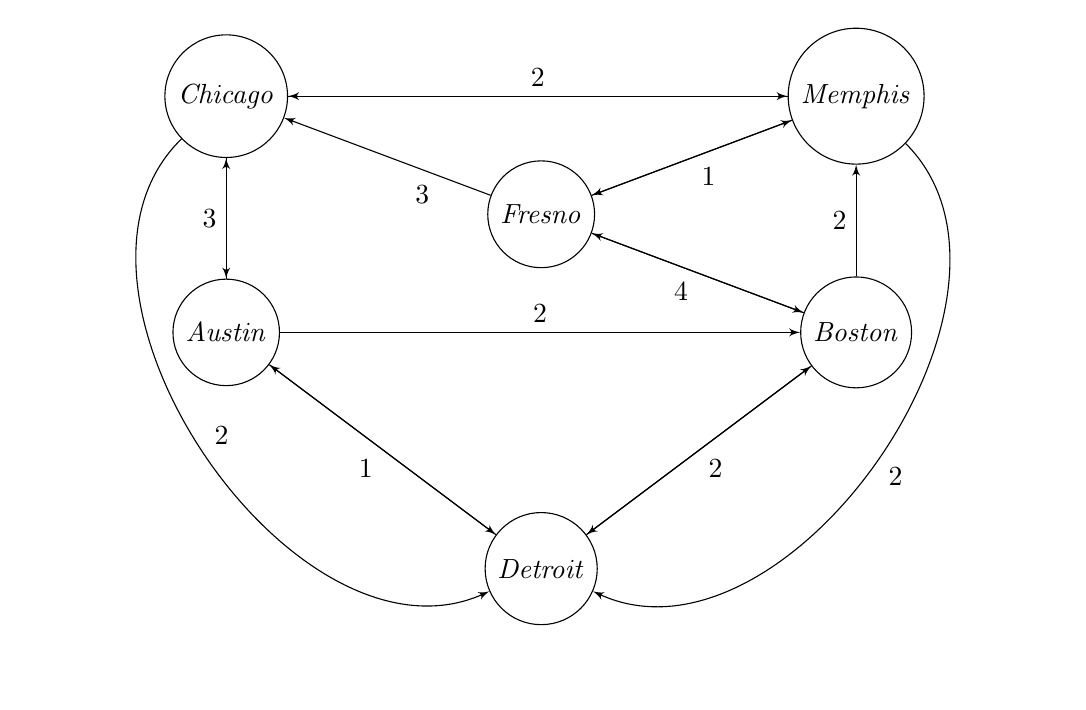
\begin{tikzpicture}
\tikzset{vertex/.style = {shape=circle,draw,minimum 
size=1.5em}}
\tikzset{edge/.style = {->,> = latex'}}
% vertices
\node[vertex] (a) at  (0,0) {$\mathit{Chicago}$};
\node[vertex] (b) at  (4,-6) {$\mathit{Detroit}$};
\node[vertex] (c) at  (8,0) {$\mathit{Memphis}$};
\node[vertex] (d) at  (8,-3) {$\mathit{Boston}$};
\node[vertex] (a1) at (0,-3) {$\mathit{Austin}$};
\node[vertex] (a2) at (4,-1.5) {$\mathit{Fresno}$};
%edges
\draw[edge] (a) to [bend right=80pt] node [auto] {2} (b);
\draw[edge] (a) to (a1);
\draw[edge] (a) to node [auto] {2} (c);
\draw[edge] (b) to (d);
\draw[edge] (b) to node [auto] {1} (a1);
\draw[edge] (c) to (a);
\draw[edge] (c) to node [auto] {1} (a2);
\draw[edge] (c) to [bend left=80pt] node [auto] {2}(b);
\draw[edge] (d) to node [auto] {2} (c);
\draw[edge] (d) to node [auto] {4} (a2);
\draw[edge] (d) to node [auto] {2} (b);
\draw[edge] (a1) to node [auto] {3} (a);
\draw[edge] (a1) to node [auto] {2} (d);
\draw[edge] (a1) to (b);
\draw[edge] (a2) to node [auto,near start] {3} (a);
\draw[edge] (a2) to (c);
\draw[edge] (a2) to (d);
\end{tikzpicture}
\end{center}
\caption{Graph of the cities}
\end{figure}
The \hex{}-program for the Travelling salesperson problem is 
encoded as follows:
\begin{exmp}
\label{travellingsalesperson}
\begin{align*}
\rowprefix{r_1} & startingCity(austin).\\
\rowprefix{r_2} & budgetB(11).\\
\\
\rowprefix{r_3} & \mathit{cityOfDegree(P,0,P,0)} \leftimpl 
\mathit{startingCity(P).} \\
& \\
\rowprefix{r_4} & \mathit{cityOfDegree(F1, DegPlus, F2, Cost)} 
\leftimpl \mathit{cityOfDegree(\_, Deg, F1, \_)}, \\ 
&\ext{edges}{F1}{F2, Cost}, \mathit{DegPlus=DegPlus+1}, 
DegPlus < 4, \\ & \#int(DegPlus), \#int(Deg)), \#int(Cost). 
\\
\rowprefix{r_5}& \mathit{node(Y)} \leftimpl 
\mathit{cityOfDgree(X, V, Y, C)}.\\
\rowprefix{r_6}& \mathit{edge}(X, Y) \leftimpl 
\mathit{cityOfDegree(X, V, Y, C).} \\
\rowprefix{r_7} & cost(X,Y,C) \leftimpl cityOfDegree(X, V, Y, C). 
\end{align*}
\begin{align*}
\rowprefix{r_8} & \{ cycle(X,Y) : edge(X,Y) \} = 1 \leftimpl 
node(X). \\
\rowprefix{r_9} &  \{ cycle(X,Y) : edge(X,Y) \} = 1 \leftimpl 
node(Y). \\
& \\
\rowprefix{r_{10}} & costCalculated(X) \leftimpl \#sum \{C,X,Y : 
cycle(X,Y), cost(X,Y,C)\} = X \\
\rowprefix{r_{11}} & withinBudget(B,C) \leftimpl budget(B), 
costCalculated(C), B \geeq C. \\
\rowprefix{r_{12}} & \leftimpl  budgetB(B), costCalculated(C), 
\nott \thinspace \mathit{withinBudget(B,C).} \\
& \\
\rowprefix{r_{13}} & reached(Y) \leftimpl cycle(C, Y), startingCity(C). \\
\rowprefix{r_{14}} & reached(Y) \leftimpl cycle(X,Y), 
reached(X). \\
\rowprefix{r_{15}} & \leftimpl node(Y), \nott \thinspace 
\mathit{reached(Y)}. \\
& \\
\rowprefix{r_{16}} & :\sim cycle(X,Y), cost(X,Y,C). [C:1] 
\end{align*}
\end{exmp}
In rule $\row{r_1}$ we have a fact which specifies the starting 
city. 
It is important to notice that in our program the starting 
point for the travelling salesperson may change and it is not 
fixed. The salesperson should start his trip from the 
city specified by the fact from $\row{r_1}$ and also finish 
his trip there if there is such a cycle which covers all 
other cities in the graph. Rule $\row{r_2}$ is a fact which defines the 
available budget of the salesperson. An atom $\mathit{cityOfDegree(R,D,S,C)}$ keeps 
track of the cities newly discovered defined as successor 
nodes $S$ for the root node $R$, their distances from the 
root node as $D$ and the weight of the edge between $R$ and $S$ 
denoted as $C$. Rule $\row{r_3}$ defines the starting city for 
the path candidate. Rule $\row{r_4}$ is responsible for 
generating a graph of 
the cities discovered. It is using the external atom 
$\mathit{\&edges}$ to load new cities from the external 
file and use them in the program. An external atom is of 
the form $\ext{edges}{F1}{F2,Cost}$ where $\mathit{F1}$ 
represents the predecessor node for which we are finding 
all successor 
nodes. $\mathit{F2}$ returns all successor nodes of 
$\mathit{F1}$ and $\mathit{Cost}$ is an integer value which 
represents weight of the edge between $\mathit{F1}$ and 
$\mathit{F2}$. $\mathit{DegPlus}$ is here set to be 4, which means we can go at most three edges far from the root node. 
There are many advantages of using an external atom of this
type:
\begin{itemize}
\item The graph may be very large and it is not possible to load it 
at once as a set of edges specified manually.
\item We do not know the graph completely (e.g., due to limited capabilities of a web service).
\item We want to analyze only a subgraph of the graph that is 
reachable from the node specified.
\end{itemize}    
In $\row{r_5}$, $\row{r_6}$ and $\row{r_7}$ the program is extracting 
$\mathit{nodes}, \mathit{edges}$ and $\mathit{costs}$ of 
the edges from the $\mathit{cityOfDegree}$ atoms. 

The rules $\row{r_8}$ and $\row{r_9}$ assert that every 
node must have exactly one outgoing and exactly one 
incoming edge, respectively, belonging to the cycle. The meaning of the two rules is described before in Section 
\ref{conditions}.

In $\row{r_{10}}$ we use aggregates (cf. Section 
\ref{aggregates}) to find the sum $X$ of the costs over the 
$\mathit{cycle(X,Y)}$. In rule $\row{r_{11}}$, an atom 
$\mathit{withinBudget(B,C)}$ is true if the term of the 
$\mathit{costCalculated(C)}$ is less than or equal to the 
term of $\mathit{budgetB(B)}$ available. The integrity 
constraint $\row{r_{12}}$ ensures that in the answer 
set overall sum of the costs for the cycle will be less 
than or equal to the budget available. The same rules can be applied to limit length travelled or time spent.

Rules $\row{\row{r_{13}}}$ and $\row{r_{14}}$ check whether all 
nodes 
are reached by a cycle candidate produced by the rules 
$\row{r_8}$ and $\row{r_9}$.  Note that rule $\row{r_8}$ builds on the
assumption that the cycle starts at city Austin. The second 
rule in $\row{r_9}$ states that, from a reached node $X$, an 
adjacent node $Y$ can be reached via a further edge in the 
cycle. It makes sure that all nodes will be reached with the 
cycle given \cite{gkklorst2015}. The integrity constraint $\row{r_{15}}$ 
eliminates answer sets where not all nodes in the graph are reached.

In order to minimize costs, we add the following 
optimization statement: \\
\centerline{$:\sim cycle(X,Y), cost(X,Y,C). \  [C:1].$}
Here, edges belonging to the cycle are weighted according 
to their costs and \dlvhex{} lists optimal answer sets only.

\subsubsection{Problem Solution}
For this example optimal answer set 
is as follows:
\begin{align*}
\{&  cycle(austin,boston), 
cycle(boston,memphis),cycle(detroit,austin), \\
& cycle(chicago,detroit), 
cycle(memphis,fresno),cycle(fresno,chicago) \} \\
& <[11:1]>.
\end{align*}
Note that we omitted input facts and intermediate results from the answer and show only the atoms specifying the final tour (optimal) to make 
answer set easier to read. The route which satisfies all given constraints is: Austin $\rightarrow$ Boston $\rightarrow$ Memphis $\rightarrow$ Fresno $\rightarrow$ Chicago $\rightarrow$ Detroit $\rightarrow$ Austin with the minimum cost of 11. 




\subsection{Example 3}
\label{example3}
The last example is from the group of pathfinding problems and it considers pathfinding for multiple agents.
 
\subsubsection{Problem Instance}
Pathfinding for a single agent is the problem of planning a 
route from an initial
location to a goal location in an environment, going around 
obstacles. 
Pathfinding for multiple agents also aims to plan such 
routes for each agent, 
subject to different constraints, such as restrictions on 
the length of each path 
or on the total length of paths, no self-intersecting 
paths, no intersection of 
paths/plans, no crossing/meeting each other.  It also has 
variations for finding optimal solutions, e.g., with 
respect 
to the maximum path length, or the sum of plan lengths. 
These problems are important
for many real-life applications, such as motion planning, 
vehicle routing, environmental monitoring, patrolling, 
computer games \cite{ekos2013}. We consider the 
problem 
where multiple agents need to find paths 
from their respective starting locations to their goal 
locations, ensuring that 
paths do not collide with static obstacles and that no two 
agents collide with 
each other. 

\subsubsection{Problem Encoding}
The \hex-program for the problem introduced in the previous 
subsection is as follows:
\begin{exmp}
\label{pathfindingAgent}
\begin{align*}
\rowprefix{r_1} & startingNode(one). \\
\rowprefix{r_2} & nodeOfDegree(P,0,P) \leftimpl startingNode(P). 
\\
\rowprefix{r_3} & nodeOfDegree(F1, DegPlus, F2) \leftimpl 
nodeOfDegree(\_, Deg, F1), \\ & \ext{edges}{F1}{F2}, 
DegPlus=Deg+1, DgPlus <= 5, \#int(DegPlus), \\ &\#int(Deg). 
\\
\rowprefix{r_4} & node(Y) \leftimpl nodeOfDegre(X, V, Y).  \\
\rowprefix{r_5} & edge(X,Y) \leftimpl nodeOfDegree(X,V,Y).\\
\\
\rowprefix{r_6} &  \mathit{agent(1). } \ \mathit{ agent(2). }\\
\rowprefix{r_7} & \mathit{start(1,one).} \ \mathit{ 
start(2,four).} \\
\rowprefix{r_8} & \mathit{goal(1,ten).} \ \mathit{ 
goal(2,eleven).} \\
\\
\rowprefix{r_9} & clear(V) \leftimpl \mathit{node(V)}, V \neq 
\mathit{three}\\ 
\\
\rowprefix{r_{10}} & guessPath(I,0,V) \leftimpl start(I,V). \\
\rowprefix{r_{11}} &  \mathit{guessPath(I, TPlus, U)} \vee 
\mathit{nguessPath(I, TPlus, U)} \leftimpl 
\mathit{agent(I)}, \\ &  \mathit{guessPath(I, T, V)},  
\mathit{edge(U,V)}, \mathit{TPlus=T+1}, 
\mathit{\#int(TPlus)}, \mathit{\#int(T).}  \\
\rowprefix{r_{12}} &  \leftimpl 1 \neq \mathit{\#count\{ U 
\colon guessPath(I, T, U) \}}, \mathit{agent(I)}, 
\mathit{\#int(T)}.  \\
\\
\row{\row{r_{13}}} \colon &  visit(I, V) \leftimpl guessPath(I,T,V). \\
\\
\rowprefix{r_{14}} & \leftimpl goal(I, V), \nott \thinspace  
\mathit{visit(I, V).} \\
\rowprefix{r_{15}} &  \leftimpl guessPath(I, T, V), 
path(I^{\prime},T,V), X \lesseq XP. \\
\rowprefix{r_{16}} &  \leftimpl guessPath(I,T,V), \nott \thinspace  
\mathit{clear(V).}\\
\\
\rowprefix{r_{17}} &  \mathit{path(I,V,U,T,ValidOrNot)} 
\leftimpl \mathit{agent(I)}, \\ & \mathit{guessPath(I, T, 
V)}, \mathit{guessPath(I, TPlus, U)}, \\ & \ext{check}{U, 
V, T, I}{ValidOrNot}, \mathit{TPlus=T+1}, \#int(T), 
\#int(TPlus).  \\
\rowprefix{r_{18}} & \leftimpl path(I, V, U, T, invalid). 
\end{align*}
\end{exmp}


In the first part of the program we load the graph using 
the $\&edges$ external atom. This atom cyclically discovers 
nodes and edges from the external file. In $\row{r_4}$ we 
extract node $Y$ whenever an atom $\mathit{nodeOfDegree(X, 
V, Y)}$ is true. Similar as in the previous rule $\row{r_5}$ extracts an edge from $X$ to $Y$ if an atom 
$\mathit{nodeOfDegree(X, V,Y)}$ is true. 

From $\row{r_6}$ to $\row{r_8}$ we define a set of facts. 
The facts $\row{r_6}$ represent different agents in the program. 
Facts $\row{r_7}$ and $\row{r_8}$ define initial and 
destination nodes for the agents.  

Rule $\row{r_9}$ 
represents that vertex $V$ is free and does not have any 
obstacle on it. Rules $\row{r_{10}}$, $\row{r_{11}}$ and 
$\row{r_{12}}$ guesses the next node to be visited by the agent, from 
node $U$ to the node $V$. The agent can either visit a new node 
using an existing edge or stay at the same node and wait. 
In rule $\row{r_{10}}$, the initial location for the path is set. Rule $\row{r_{11}}$ 
with a disjunctive head (cf. Section~\ref{disjunction}) decides either to include the outgoing edge 
from the node $U$ to the path or to omit it from the path. 
This step is cyclically performed until the goal nodes are not 
reached. The constraint $\row{r_{12}}$ eliminates all answer sets in which there is more than one outgoing edge 
selected at some time point from node $U$. Thus, for each step 
the agent has to select a single edge since it cannot be at the 
two different locations at the same time. Rule $\row{\row{r_{13}}}$ computes which nodes are visited using the path 
guessed. The integrity constraint $\row{r_{14}}$ ensures that 
each agent reaches its destination node. We ensure that 
agents do not collide with each other using constraint 
$\row{r_{15}}$. We also ensure that agents do not go through 
obstacles using constraint $\row{r_{16}}$. 

We represent path plans by atoms of the form 
$\mathit{path(I, V, U, T, ValidOrNot)}$ which specify that 
at time step $T$, agent $I$ moves from a node $V$ to a 
node $U$. An external atom is used to decide whether that move is valid or invalid. The last 
two rules $\row{r_{17}}$ and $\row{r_{18}}$ check if the overall path is valid or invalid. Agents can only know what are the edges 
available in the graph and make the guess in which 
direction they should go. Consider that an agent selects 
some 
edge but it becomes unusable because of some reasons in the meantime. 
The reasons may be obstacles in the environment, too narrow corners, too small doors or any change on 
the graph or on the environment which is not considered as 
a fact in the program. By introducing this property we have a dynamic problem. To perform this check we 
can use only an external source. The external source is of the 
form \ext{check}{U,V,T,I}{ValidOrNot} and checks is the 
guessed move of the agent $I$ from $U$ to $V$ at time $T$ is 
$\mathit{valid}$ or $\mathit{invalid}$. In the case that 
any of the moves in the guessed path is invalid, the whole 
answer set is eliminated. If no invalid moves are guessed in the path, it means that solution is the answer set of the program.            

\subsubsection{Problem Solution} 
Let us solve the problem using the following graph.  
\begin{figure}
\begin{center}
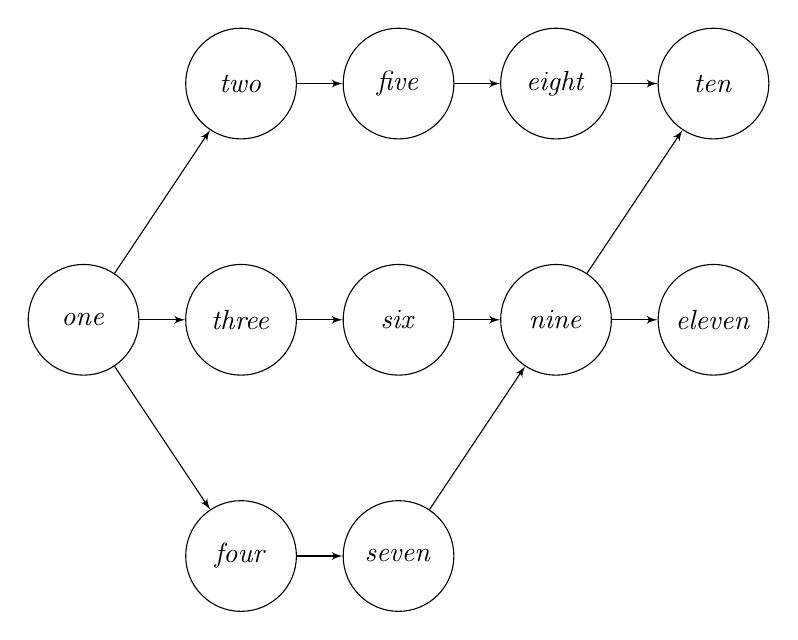
\begin{tikzpicture}
\tikzset{vertex/.style = {shape=circle,draw,minimum 
size=4em}}
\tikzset{edge/.style = {->,> = latex'}}
% vertices
\node[vertex] (a) at  (0,3) {$\mathit{one}$};
\node[vertex] (b) at  (2,6) {$\mathit{two}$};
\node[vertex] (c) at  (2,3) {$\mathit{three}$};
\node[vertex] (d) at  (2,0) {$\mathit{four}$};
\node[vertex] (e) at  (4,6) {$\mathit{five}$};
\node[vertex] (f) at  (4,3) {$\mathit{six}$};
\node[vertex] (g) at  (4,0) {$\mathit{seven}$};
\node[vertex] (i) at  (6,6) {$\mathit{eight}$};
\node[vertex] (j) at  (6,3) {$\mathit{nine}$};
\node[vertex] (k) at  (8,6) {$\mathit{ten}$};
\node[vertex] (l) at  (8,3) {$\mathit{eleven}$};
%edges
\draw[edge] (a) to (b);
\draw[edge] (a) to (c);
\draw[edge] (a) to (d);
\draw[edge] (b) to (e);
\draw[edge] (c) to (f);
\draw[edge] (d) to (g);
\draw[edge] (e) to (i);
\draw[edge] (f) to (j);
\draw[edge] (g) to (j);
\draw[edge] (i) to (k);
\draw[edge] (j) to (l);
\draw[edge] (j) to (k);
\end{tikzpicture}
\end{center}
\caption{Simulation of the environment used by agents}
\end{figure}
The graph is again loaded from the external file and not 
specified as a set of facts. We know that there is an obstacle at node $\mathit{three}$, so any answer set with node 
$\mathit{three}$ in the path is removed. All other 
constraints must be satisfied as well. Note that we have 
omitted most of the atoms in order to emphasize the actual 
solution (in order to see how to filter out answer sets and 
show only specific atoms at the output refer to the 
Section~\ref{sec:commandline}; in our answer set, we are 
interested only in $\mathit{path}$ atoms since we want to 
see what is the path from the initial node $U$ to the 
destination node $V$). One answer set is as follows:
\\Answer Set 1:
\begin{align*}
\{ & path(1,one,two,0,valid), path(1,two,five,1,valid),
\\ & path(1,five,five,2,valid), path(2,four,four,0,valid),
\\ & path(2,four,seven,1,valid), 
path(1,five,eight,3,valid),
\\ & path(2,seven,nine,2,valid), path(1,eight,ten,4,valid),
\\ & 
path(2,nine,eleven,3,valid),path(2,eleven,eleven,4,valid) 
\}
\end{align*} 
Here, $\mathit{agent(1)}$ follows the path:
one $\rightarrow$ two $\rightarrow$ five $\rightarrow$ five 
$\rightarrow$ eight $\rightarrow$ ten. At each time 
point an agent chooses either to wait or to move to 
the another node. At $t=2$ the $\mathit{agent(1)}$ chooses 
to wait and not to move. The same logic is applied for the 
$\mathit{agent(2)}$. To show different possible choices we are 
giving two answer sets more:
\\Answer Set 2:
\begin{align*}
\{ & path(1,one,two,0,valid),path(1,two,five,1,valid),
\\ & path(1,five,five,2,valid),path(2,four,seven,0,valid),
\\ & path(1,five,eight,3,valid),path(2,seven,nine,1,valid),
\\ & path(2,nine,nine,2,valid),path(1,eight,ten,4,valid),
\\ & 
path(2,nine,eleven,3,valid),path(2,eleven,eleven,4,valid)\}
\end{align*}
In the second answer set, the path for the first agent did not 
change. However, the second agent changes its path and instead 
of waiting at $t=0$ at node four it moves to the node 
seven.  
\\Answer Set 3:
\begin{align*}
\{ & path(1,one,four,0,valid), path(1,four,seven,1,valid),
\\ & path(1,seven,nine,2,valid), path(2,four,seven,0,valid),
\\ & path(2,seven,nine,1,valid), 
path(1,nine,ten,3,valid),
\\ & path(2,nine,eleven,2,valid), path(1,ten,ten,4,valid),
\\ & 
path(2,eleven,eleven,3,valid),path(2,eleven,eleven,4,valid) 
\}
\end{align*} 

\section{External Interfaces}
\label{sec:externalInterfaces}
This section discusses the implementation of external sources. One important design principle was to provide a 
mechanism to easily add further external atoms, as introduced in Section~\ref{extatoms}, without 
having to recompile the main application.
 
Formally, an external atom is defined to evaluate to true
or false, depending on a number of parameters:
\begin{itemize}
\item An interpretation (a set of atoms)
\item A list of input constants
\item A list of output constants
\end{itemize}  
However, it is more intuitive and convenient to think of an 
external atom not as being boolean, but rather functional:
depending on a given interpretation and a list of input 
constants, it returns output tuples for which it is true. For instance, the 
external atom to import triples from RDF files has the 
form: \\
\centerline{$\ext{rdf}{uri}{X,Y,Y}$} 
where $\mathit{uri}$ stands for a string denoting the RDF-source and X,Y, and Z are variables that represent an RDF-triples from the specified source.

\subsection{Information Flow}
The interface that is used by \dlvhex{} to access a plugin 
follows very closely this semantics. For each atom, a 
retrieval function has to be implemented, which receives a 
query object and has to return an answer-object. The 
query object carries the input interpretation as well as 
the ground input parameters of the external atom call, 
while the answer object is a container for the output 
tuples of the external atom's function.   

\subsection{Types of Input Parameters}
In practice, only 
parts of the interpretation might be needed. Considering 
this as well as for efficiency reasons, there are three types of input parameters: 
\begin{itemize}
\item Constant parameters
\item Predicate parameters
\item Tuples
\end{itemize}

A parameter of type \emph{constant} is not related to the 
interpretation at all, like in the previous example of the 
RDF-atom where we have strings as a constant input to the external atom. 

A parameter is of type \emph{predicate} means that 
all atoms in the interpretation with this predicate are 
necessary for the external atom. Let us assume, we have an external 
atom that calculates the overall price of a number of books 
given by their ISBN number:\\
\centerline{$\ext{overallbookprice}{isbn}{X}$}
The single input parameter of this atom would be of type 
\emph{predicate}, meaning that not the constant itself is 
necessary for the atom's function, but the part of the 
interpretation with this predicate. So if we have, e.g.,\\ 
I = \{$\mathit{isbn(``0}$-$\mathit{19}$-$\mathit{82183}$-$\mathit{6")}$, $ \mathit{isbn(``0}$-$\mathit{201}$-$\mathit{99954}$-$\mathit{4")}$, $p(a)$, $q(b)$ $\dots$ \}
the atom's function will be called with the filtered interpretation: \\
$I=$\{$\mathit{isbn(``0}$-$\mathit{19}$-$\mathit{82183}$-$\mathit{6")}$, $ \mathit{isbn(``0}$-$\mathit{201}$-$\mathit{99954}$-$\mathit{4")}$\}

A parameter of type \emph{tuple} represents a meta category standing for an arbitrary number of constant input parameters. This is useful when we have to send multiple constant parameters separately, e.g., for \\
\centerline{$\ext{concat}{string1, string2, string3, \dots}{Out}$}. 

Specifying the type of input parameters not only helps to 
single out the relevant part of the interpretation, but 
also supports \dlvhex{} in calculating the dependencies 
within a \hex-program. Plugins can be implemented either in Python or C++, as shown in the following two subsections.

\subsection{Python}
With \dlvhex{} version 2.4.0, a Python plugin interface was 
introduced, which supports Python scripts that provide 
functions to realise custom external atoms. For every Python plugin two tasks are to be carried out:
\begin{itemize}
\item Write a new Python script which contains a register function and imports the package \dlvhex{}.
\item Write another function for each external atom, and export this function using the $\mathit{register}$ function. 
\end{itemize}
The \verb+register+ function has the following form:
\begin{verbatim} 
def register():
  dlvhex.addAtom("Atom_Name",(Input_Parameters),Output_Arity) 
\end{verbatim}
It contains a call of \verb+addAtom+ for each external atom. Each call specifies a tuple of arity 3:
\begin{itemize}
\item \verb+Atom_Name+ is the name of the 
external predicate.
\item \verb+Input_Parameters+ is a tuple of arbitrary many input parameter types. Each input parameter type is one of the 
following: \verb+dlvhex.CONSTANT+, \verb+dlvhex.PREDICATE+ or 
\verb+dlvhex.TUPLE+, as it is introduced in the previous section.
\item \verb+Output_Arity+ is an integer value representing the output arity of an atom.  
\end{itemize}
Consider the $\mathit{\&concat}$ external atom which we introduced in the previous section. It takes two strings as input and outputs their concatenation. The register function then would be as follows:
\begin{verbatim}
def register():
  dlvhex.addAtom("concat", (dlvhex.CONSTANT, dlvhex.CONSTANT), 1)  
\end{verbatim}
Once the external atom is registered successfully, it has 
to be implemented in the form of another Python function 
with an appropriate number of input parameters. It has the 
following form:  
\begin{verbatim}
def Atom_Name(Input_Parameter_1, Input_Parameter_2, ...)
  dlvhex.output((Output_Parameter_1, ...))
\end{verbatim}

The implementation of the \verb+concat+ function is as follows:
\begin{verbatim}
def concat(a,b)
  # Function body goes here
  dlvhex.output((str, ))
\end{verbatim} 
To get more familiar with Python plugins we are providing three examples as there are three possible input parameter types.

The plugin in Example~\ref{constantAsInput} uses a constant (string) input parameter. It is used in Example~\ref{faceQuery} to query all direct friends of the person of interest.
\begin{exmp}
\label{constantAsInput}
\begin{verbatim}

1:  import dlvhex
2:  import networkx as nx

3:  def friendsOf(personOfInterest):
4:    g = nx.read_weighted_edgelist("test.edgelist",nodetype=str,
                                    create_using=nx.DiGraph())
5:    friendList = g.successors(personOfInterest.value())
6:    for item in friendList:
7:      dlvhex.output((item, ))

8:  def register():
9:  prop = dlvhex.ExtSourceProperties()
10: prop.addFiniteOutputDomain(0)
11: dlvhex.addAtom("friendsOf", (dlvhex.Constant, ),1,prop)
\end{verbatim}
\end{exmp}

In the lines 1 and 2 we have imported two libraries which 
are required. We have to import the \verb+dlvhex+ 
library as for every plugin. The \verb+networkx+ library is needed in this particular example since we are 
performing graph operations (i.e. loading graphs from the file, get all successors of the node etc). 

Lines \verb+3+ to \verb+7+ implement the \verb+friendsOf+ external atom. 
It receives the name of the person as string and searches for all 
direct friends of that person in the graph, which is loaded from the file in line \verb+4+. All discovered friends, are output in line \verb+7+. 

Lines \verb+8+ to \verb+11+ register the external atom 
\verb+friendsOf+ with constant input parameter and 
single output parameter. 

The following example uses a predicate input parameter 
for the \verb+&rq+ external atom as used in Example~\ref{swimExample}. The external atom is performing 
a Web search to check the requirements for the selected location. It is of the form 
$\ext{\mathit{rq}}{\mathit{location\_choice}}
{\mathit{required\_resource}}$ which intuitively evaluates 
to true if a given location\_choice requires a certain 
required\_resource and represents such resources and their 
origin (inoutd, or loc) using predicate $\mathit{need}$. 
\begin{exmp}
\label{predicateAsInput}
\begin{verbatim}

1:  import dlvhex 

2:  def rq(location_chioce)
3:    for x in dlvhex.getTrueInputAtoms():
4:      io = {"ind":"money","amalB":"goggles","altD":"yogamat",
              "gansD":"money"}
5:      if location_chioce == x.tuple()[0]:
6:        inp = x.tuple()[1].value()
7:          if inp in io:
8:            dlvhex.output((io[inp], ))

9:  def register():
10:   dlvhex.addAtom("rq", (dlvhex.PRDICATE), ), 1)
\end{verbatim}
\end{exmp}

From line \verb+2+ to line \verb+8+ we implement the \verb+rq+ function. Line \verb+5+ filters the atoms according to the given predicate. In Line 6 we check if the predicate of the current input atom is equivalent to \texttt{location\_choice}, which specifies the selected location. Line \verb+8+ is returning  
the requirements (if any) of the location specified by variable 
\verb+inp+. Lines \verb+9+ to \verb+10+ define the register 
function for the \verb+rq+ external atom.

As mentioned above, there exists a third parameter type \emph{tuple}. It stands for an arbitrary number of constant input parameters. The following example presents the usage of a tuple in a plugin used to implement string concatenation for arbitrary many strings.  
\begin{exmp}
\label{tupleAsInput}
\begin{verbatim}

1:  import dlvhex

2:  def concat(tup):
3:    ret=" "
4:    for x in tup:
5:      ret = ret + x.value()
6:    dlvhex.output((ret, ))

7:  def register():
8:    dlvhex.addAtom("concat", (dlvhex.TUPLE, ), 1)
\end{verbatim}
\end{exmp}
This plugin receives a tuple of strings, concatenates 
them and outputs them as a single string value. The function \verb+concat+ is implemented from line \verb+2+ to \verb+6+. In line \verb+3+, an 
empty string is initialized. Inside the for loop, the input 
strings are appended to the string initialized. This process 
is continued until all strings from the tuple have been processed.  
 
A more detailed description of all methods available for the \dlvhex{} Python module can be found at:\\ \url{http://www.kr.tuwien.ac.at/research/systems/dlvhex/doc2x/}\\
\url{group__pythonpluginframework.html}
\subsection{C++}
TODO

\section{Command Line options}
\label{sec:commandline}
In this section, we briefly describe the meaning of the command line options supported by \dlvhex{}. 
Calling only \dlvhex{} without any arguments will show all 
command line options available. For each option, we indicate whether it requires an argument, and if so, we also describe its meaning. An abstract invocation of \dlvhex{} looks as follows:\\
\texttt{dlvhex2 [OPTION] FILENAME [FILENAME ...]} or \texttt{dlvhex2 [OPTION] --}

\bigskip
The following set of commands is related with Input, Output and  Reasoning options and they directly affect the result.
% Sets column space
%\def\arraystretch{2}\tabrowsep=50pt
% Sets row space
\renewcommand{\arraystretch}{1.6}
\begin{longtable}{p{2.2cm}  p{2.5cm} p{0.6cm} p{6.3cm}  } 
 & \texttt{--}& & Parse from standard input. \\ 
\texttt{-s} & \texttt{--silent}&& Do not display anything than the actual result \\ 
\texttt{-f} & \texttt{--filter=foo[,bar[,...]]} && \\
& & & Only display instances of the specified predicate(s).\\
& \texttt{--nofacts} && Do not output EDB facts. EDB facts are the facts of the program.  \\
\texttt{-n} & \texttt{--number=<num>} && Limit number of displayed models to $\langle$\texttt{num}$\rangle$, Default value is 0, which means to display all models.\\ 
\texttt{-N} & \texttt{--maxint=<num>} && Set maximum integer (\# \texttt{maxint} in the program takes precedence). \\
 & \texttt{--weaksafety} && Skip strong safety check.\\
 & \texttt{--strongsafety} && Applies traditional strong safety criteria. \\
  & \texttt{--liberalsafety} && Uses more liberal safety condition than strong safety. \\
  &\texttt{--mlp}&& Use \dlvhex{}$+$mlp solver (modular nonmonotonic logic programs).\\
  & \texttt{--forget} && Forget previous instantiations that are not involved in current computation (mlp setting). \\
  & \texttt{--split} &&Use instantiation splitting techniques.\\
  & \texttt{--noeval} && Parse the program, but do not evaluate it (only useful with \texttt{--verbose}). \\
  & \texttt{--keepnsprefix} && Keep specified namespace-prefixes in the result. \\
  & \texttt{--keepauxpreds} && Keep auxiliary predicates in answer sets. \\
\end{longtable}
\bigskip
\subsection{Plugin Options}
\begin{center}
\begin{tabular}{p{2.2cm}  p{2.5cm} p{0.6cm} p{6.3cm}  } 
 \texttt{-p}&\texttt{--plugindir=DIR}&&Specify additional directory where to look for plugin libraries (additionally to the installation plugin-dir and \texttt{\$HOME/.dlvhex/plugins}). Start with \texttt{!} to reset the preset plugin paths, e.g., ``\texttt{!:/lib}'' will use only \texttt{/lib/}.
 \\
\end{tabular}
\end{center}

\subsection{Performance Tuning Options}
\begin{center}
\begin{longtable}{p{0.7cm}  p{2.2cm} p{0.3cm} p{6.3cm}  } 
%--EXTLEARN
\multicolumn{4}{p{6cm}}{\texttt{--extlearn[=none,iobehavior,monotonicity,functionality,}} \\[-1.5ex]
&& \multicolumn{2}{l}{\texttt{linearity,neg,user,generalize]}} \\
& & & Learn nogoods from external atom evaluation (only useful with \texttt{--solver=genuineii} or \texttt{--solver=genuinegi)}.\\
&\texttt{none}:& & Deactivate external learning. \\
&\texttt{iobehaviour}:& &Apply generic rules to learn input-output behaviour. \\
&\texttt{monotonicity}:& &Apply special rules for monotonic and antimonotonic external atoms.\\
&\texttt{functionality}:& &Apply special rules for external atoms which are linear in all predicate parameters.\\
&\texttt{linearity}:& &Apply special rules for external atoms which are linear in all predicate parameters.\\
&\texttt{neg}:& &Learn negative information\\
&\texttt{user}:& &Apply user-defined rules for nogood learning\\
&\texttt{generalize}:& &Generalize learned ground nogoods to ground nogoods.\\
& & & By default all options above except ``\texttt{generalize}'' are enabled.\\
%%%%%%%%%%%%%%%%%%%
\multicolumn{4}{l}{\texttt{--supportsets}}\\
& & &Exploits support sets for evaluation.\\
%%%%%%%%%%%%%%%%%%%
\multicolumn{4}{l}{\texttt{--evalall}}\\
& & &Evaluate all external atoms in every compatibility check, even if previous external atoms already failed.  This makes nogood learning more independent of the sequence of external atom checks. Only useful with \texttt{--extlearn}.\\
%%%%%%%%%%%%%%%%%%%
\multicolumn{4}{l}{\texttt{--nongroundnogoods}}\\
& & &Automatically instantiate learned nonground nogoods.\\
%%%%%%%%%%%%%%%%%%%
\multicolumn{4}{l}{\texttt{--flpcheck=[explicit,ufs,ufsm,aufs,aufsm,none]}}\\
& & &Sets the strategy used to check if a candidate is a subset-minimal model of the reduct.\\
&\texttt{explicit}:&&Compute the reduct and compare its models with the candidate\\
&\texttt{ufs}:&&Use unfounded sets for minimality checking
\\
&\texttt{ufsm}:&&Use unfounded sets for minimality checking, do not decompose the program for UFS checking.\\
&\texttt{aufs (default)}:&&Use unfounded sets for minimality checking by exploiting assumptions\\
&\texttt{aufs}:&&Use unfounded sets for minimality checking by exploiting assumptions. Do not decompose the program for UFS checking.\\
&\texttt{none}:&&Disable the check.\\
%%%%%%%%%%%%%%%%%%%
\multicolumn{4}{l}{\texttt{--flpcriterion=[all,head,e,none]}}\\
& & & Defines the kind of cycles whose absence is exploited for skipping minimality checks.\\
&\texttt{all (default)}:&&Exploit head- and e-cycles for skipping minimality checks\\
&\texttt{head}:&& Exploit head-cycles for skipping minimality checks\\
&\texttt{e}:&&Exploit e-cycles for skipping minimality checks\\
&\texttt{none}:&& Do not exploit head- or e-cycles for skipping minimality checks\\
%%%%%%%%%%%%%%%%%%%
\multicolumn{4}{l}{\texttt{--noflpcriterion}}\\
& & & Do no apply decision criterion to skip the FLP check. (equivalent to \texttt{--flpcriterion=none)}\\
\multicolumn{4}{l}{\texttt{--ufslearn=[none,reduct,ufs]}}\\
& & & Enable learning from UFS checks (only useful with \texttt{--flpcheck=[a]ufs[m]}).\\
&\texttt{none}:&&No learning\\
&\texttt{reduct}:&&Learning is based on the FLP-reduct\\
&\texttt{ufs (default)}:&&Learning is based on the unfounded set\\
%%%%%%%%%%%%%%%%%%%
\multicolumn{4}{l}{\texttt{--eaevalheuristics=[always,periodic,inputcomplete,}}\\
\multicolumn{4}{l}{\texttt{eacomplete,post,never}}\\
& & & Selects the heuristic for external atom evaluation.\\
&\texttt{always}:&&Evaluate whenever possible\\
&\texttt{periodic}:&&Evaluate in regular intervals.\\
&\texttt{incomplete}:&&Evaluate whenever the input to the external atom is complete\\
&\texttt{eacomplete}:&& Evaluate whenever all atoms relevant for the external atom are assigned\\
&\texttt{post (default)}:&&Only evaluate at the end\\
&\texttt{never}:&&Only evaluate at the end and also ignore custom heuristics provided by plugins\\
&&&Except for heuristics "never", custom heuristics provided by external atoms overrule the global heuristics for the particular external atom.\\
%%%%%%%%%%%%%%%%%%%
\multicolumn{4}{l}{\texttt{--ufscheckheuristic=[post,max,periodic]}}\\
& & & Specifies the frequency of unfounded set checks (only useful with \texttt{--flpcheck=[a]ufs[m])}.\\
&\texttt{post (default)}:&&Do UFS check only over complete interpretations\\
&\texttt{max}:&&Do UFS check as frequent as possible and over maximal subprograms\\
&\texttt{periodic}:&&Do UFS check in periodic intervals\\
%%%%%%%%%%%%%%%%%%%
\multicolumn{4}{l}{\texttt{--modelqueuesize=N}}\\
& & & Size of the model queue, i.e. number of models which can be computed in parallel. Default value is 5. The option is only useful for clasp solver.\\
%%%%%%%%%%%%%%%%%%%
\multicolumn{4}{l}{\texttt{--solver=S}}\\
& & & Use S as ASP engine, where S is one of \dlv{}, \dlvdb{}, \libdlv{}, \libclingo{}, \genuineii{}, \genuinegi{}, \genuineic{}, \genuinegc{} (\texttt{genuineii}=(i)nternal grounder and (i)nternal solver; \texttt{genuinegi}=(g)ringo grounder and (i)nternal solver \texttt{genuineic}=(i)nternal grounder and (c)lasp solver; \texttt{genuinegc}=(g)ringo grounder and (c)lasp solver).\\
%%%%%%%%%%%%%%%%%%%
\multicolumn{4}{l}{\texttt{--claspconfig=C}}\\
& & & If clasp is used, configure it with \texttt{C} where \texttt{C} is parsed by clasp config parser, or \texttt{C} is one of the predefined strings frumpy, jumpy, handy, crafty, or trendy.\\
%%%%%%%%%%%%%%%%%%%
\texttt{-e}& \multicolumn{3}{l}{\texttt{--heuristics=H}}\\
& & & Use \texttt{H} as evaluation heuristics, where \texttt{H} is one of\\
&\texttt{old}:&&Old dlvhex behavior\\
&\texttt{trivial}:&&Use component graph as eval graph (much overhead)\\
&\texttt{easy}:&&Simple heuristics, used for LPNMR2011\\
&\texttt{greedy (default)}:&& Heuristics with advantages for external behaviour learning\\
&\texttt{monolithic}:&& Put entire program into one unit\\
&\texttt{manual:<file>:} &&  Read ``collapse'' $\langle$ idxs $\rangle$ share $\langle$idxs$\rangle$ commands from $\langle$file$\rangle$ where component indices $\langle$idx$\rangle$ are from \texttt{--graphviz=comp}\\
&\texttt{asp:<script>}:&&Use asp program $\langle$\texttt{script}$\rangle$ as eval heuristic\\
%%%%%%%%%%%%%%%%%%%
\multicolumn{4}{l}{\texttt{--forcegc}}\\
& & & Always use the guess and check model generator.\\
%%%%%%%%%%%%%%%%%%%
\texttt{-m}& \multicolumn{3}{l}{\texttt{--modelbuilder=M}}\\
& & & Use \texttt{M} as model builder, where \texttt{M} is one of (online,offline).\\
%%%%%%%%%%%%%%%%%%%
\multicolumn{4}{l}{\texttt{--nocache}}\\
& & &Do not cache queries to and answers from external atoms.\\
%%%%%%%%%%%%%%%%%%%
\multicolumn{4}{l}{\texttt{--iauxinaux}}\\
& & &Keep auxiliary input predicates in auxiliary external atom predicates (can increase or decrease efficiency).\\
%%%%%%%%%%%%%%%%%%%
\multicolumn{4}{l}{\texttt{--constspace}}\\
& & &Free partial models immediately after using them. This may cause some models to be computed multiple times. (Not with monolithic.)\\
\end{longtable}
\end{center}
\subsection{Debugging and General Options}
\begin{center}
\begin{longtable}{p{2.2cm}  p{2.5cm} p{0.6cm} p{6.3cm}  }
%%%%%%%%%%%%%%%%%%%
\multicolumn{4}{l}{\texttt{--dumpevalplan=F}}\\
& & & Dump evaluation plan (usable as manual heuristics) to file \texttt{F}.\\
%%%%%%%%%%%%%%%%%%%
\texttt{-v}& \multicolumn{3}{l}{\texttt{--verbose[=N]}}\\
& & & Specify verbose category (if option is used without [\texttt{=N}] then default is 1):\\
&\texttt{1}:&& Program analysis informations (including dot-file)\\
&\texttt{2}:&& Program modifications by plugins\\
&\texttt{4}:&& Intermediate model generation info\\
&\texttt{8}:&& Timing information (only if configured with \texttt{\texttt{--enable-benchmark}})\\
&&&add values for multiple categories.\\
%%%%%%%%%%%%%%%%%%%
\multicolumn{4}{l}{\texttt{--dumpstats}}\\
& & & Dump certain benchmarking results and statistics in CSV format. (Only if configured with --enable-benchmark.)\\
%%%%%%%%%%%%%%%%%%%
\multicolumn{4}{l}{\texttt{--graphviz=G}}\\
& & & Specify comma separated list of graph types to export as .dot files. Default is none, graph types are:\\
&\texttt{dep}:&& Dependency Graph (once per program)\\
&\texttt{cycinp}:&& Graph for analysis cyclic predicate inputs (once per G\&C-eval unit)\\
&\texttt{comp}:&& Component Graph (once per program)\\
&\texttt{eval}:&& Evaluation Graph (once per program)\\
&\texttt{model}:&& Model Graph (once per program, after end of computation)\\
&\texttt{imodel}:&& Individual Model Graph (once per model)\\
&\texttt{attr}:&& Attribute dependency graph (once per program)\\
%%%%%%%%%%%%%%%%%%%
\multicolumn{4}{l}{\texttt{--version}}\\
& & & Shows version information.\\
%%%%%%%%%%%%%%%%%%%
\multicolumn{4}{l}{Plugin help for dlvhex-manualevalheuristicsplugin[internal]:}\\
\multicolumn{4}{l}{\texttt{--manualevalheuristics-enable}}\\
& & & Enable parsing and processing of ``\texttt{\#evalunit(...)}'' instructions.\\
%%%%%%%%%%%%%%%%%%%
\multicolumn{4}{l}{Plugin help for dlvhex-manualevalheuristicsplugin[internal]:}\\
\multicolumn{4}{l}{\texttt{--query-enable=[true,false]}}\\
& & & Enable or disable the querying plugin (default is disabled).\\
\multicolumn{4}{l}{\texttt{--query-brave}}\\
& & & Do brave reasoning.\\
\multicolumn{4}{l}{\texttt{--query-all}}\\
& & & Give all witnesses when doing ground reasoning.\\
\multicolumn{4}{l}{\texttt{--query-cautious}}\\
& & & Do cautious reasoning.\\
%%%%%%%%%%%%%%%%%%%
\multicolumn{4}{l}{Plugin help for dlvhex-aggregateplugin[internal]:}\\
\multicolumn{4}{l}{\texttt{--aggregate-enable[=true,false]}}\\
& & & Enable aggregate plugin (default is enabled).\\
%%%%%%%%%%%%%%%%%%%
\multicolumn{4}{l}{\texttt{--aggregate-mode=[native,ext]}}\\
& & & Enable aggregate plugin (default is enabled).\\
&\texttt{native (default)}:&& Keep aggregates (but simplify them to some basic types).\\
&\texttt{ext}:&& Rewrite aggregates to an external atoms.\\
%%%%%%%%%%%%%%%%%%%
\multicolumn{4}{l}{\texttt{--aggregate-allowaggextcycles}}\\
& & & Allows cycles which involve both aggregates and external atoms. If the option is not specified, such cycles lead to abortion; if specified, only a warning is printed but the models might be not minimal. With \texttt{--aggregate-mode=ext}, the option is irrelevant as aggregates are replaced by external atoms (models will be minimal in that case). See examples/aggextcycle1.hex..\\
%%%%%%%%%%%%%%%%%%%
\multicolumn{4}{l}{Plugin help for dlvhex-strongnegationplugin[internal]:}\\
\multicolumn{4}{l}{\texttt{--strongnegation-enable[=true,false]}}\\
& & & Enable or disable strong negation plugin (default is enabled).\\ 
%%%%%%%%%%%%%%%%%%%
\multicolumn{4}{l}{Plugin help for dlvhex-weakconstraintplugin[internal]:}\\
\multicolumn{4}{l}{\texttt{--weak-enable[=true,false]}}\\
& & & Enable or disable weak constraint plugin (default is enabled). \texttt{--weak-allmodels} Display all models also under weak constraints.\\ 
%%%%%%%%%%%%%%%%%%%
\multicolumn{4}{l}{Plugin help for dlvhex-functionplugin[internal]:}\\
\multicolumn{4}{l}{\texttt{--function-maxarity=<N>}}\\
& & & Maximum number of output terms in functionDecompose.\\ 
%%%%%%%%%%%%%%%%%%%
\multicolumn{4}{l}{\texttt{--function-rewrite}}\\
& & & Rewrite function symbols to external atoms.\\ 
%%%%%%%%%%%%%%%%%%%
\multicolumn{4}{l}{Plugin help for dlvhex-choicePlugin[internal]:}\\
\multicolumn{4}{l}{\texttt{--choice-enable[=true,false]}}\\
& & & Enable choice rules (default is enabled).\\
%%%%%%%%%%%%%%%%%%%
\multicolumn{4}{l}{Plugin help for dlvhex-conditionalLiteralPlugin[internal]:}\\
\multicolumn{4}{l}{\texttt{--conditinal-enable[=true,false]}}\\
& & & Enable conditional literals (default is enabled).\\
%%%%%%%%%%%%%%%%%%%
\multicolumn{4}{l}{Plugin help for dlvhex-pythonplugin[internal]:}\\
\multicolumn{4}{l}{\texttt{--python-plugin=[PATH]}}\\
& & & Add Python script "PATH" as new plugin.\\
\multicolumn{4}{l}{\texttt{--python-main=PATH}}\\
& & & Call method "main" in the specified Python script (with dlvhex support) instead of evaluating a program.\\
\multicolumn{4}{l}{\texttt{--python-arg=ARG}}\\
& & &Passes arguments to Python (sys.argv) (can be used multiple times).\\
\end{longtable}
\end{center}


\section{Input-related warnings and errors}
\label{sec:inputRelatedWarnings}
This section explains the most frequent errors, warnings, and info messages related
to inappropriate inputs or command line options. All messages are printed to the
standard error stream.

\subsection{Syntax Errors}
In this section we consider errors emitted during the parsing and checking of logic programs.
These errors include information to ease finding and fixing the problem. Each of the error messages below
shows a line in which the error appears, followed by the type of the error and a short description of the error in standard error stream.
\begin{align*}
 & \texttt{8 \ unparsed \  ``go $\leftimpl$ goto(X)'' }\\
 & \texttt{8 ----------$\widehat{}$} \\
 & \texttt{GeneralError:Syntax \ Error: \ Could \ not \ parse \ complete \ input!}
\end{align*}

To correct this error, please investigate the indicated location and make sure that the input respects the grammar as shown in Section~\ref{sec:inputLang} (like a missing period, an unmatched parenthesis,
etc.).

\subsection{Plugin-related errors}
In this section we explain exceptions and errors 
which may occur while working with external atoms 
or plugins in which we have implemented desired external atom functionality (e.g. Python or C++ plugin). 

The following exception occurs whenever we try to
load a plugin from a nonexisting file, either from the Python or C++ file.
\begin{align*}
\texttt{Exception: nonexisting\_file\_name.py : no such file}
\end{align*}
$\texttt{nonexisting\_file\_name.py}$ does not exist in the current directory and should be replaced with
the right file which contains implementation for the external atom(s) used in \hex{}-program.

The following error occurs if we do not provide an external atom specification and implementation 
in the source file but we use it in the \hex{}-program. The error looks as below:
\begin{align*}
& \texttt{GeneralError: Fatal: did not find plugin atom for predicate}\\ 
& \texttt{"ext\_atom"}
\end{align*}  
From the description above we can see that there is no plugin atom for the predicate \texttt{ext\_atom}
in the source file which is passed as parameter from the command line. Implementation for the predicate 
\texttt{ext\_atom} should be added to the plugin source file.

Another error occurs if the output arity of an external atom does not 
match its specification in the source file. The error is given below:
\begin{align*}
& \texttt{GeneralError: External Atom \ext{rq}{ind}{C,A} has a wrong} \\
& \texttt{output arity (should be 1)}
\end{align*}  

\subsection{Safety Checking}
\label{safetyCheck}
If any of the variables used in the \hex{}-program does not satisfy safety conditions listed below, the program is not safe and an error occurs. Examples and explanations in the following subsections are used from \cite{brfwilvpg2009}. 

\subsubsection{Regular Safety}
\dlvhex{} imposes a safety condition on variables in rules. 
This guarantees that a rule has only finitely many ground instances.

\paragraph{Standard, Arithmetic and Comparative Predicates}
A variable $X$ in an aggregate-free rule is safe if at least one 
of the following conditions is satisfied:
\begin{itemize}
\item $X$ occurs in a positive standard predicate in the 
body of the rule;
\item $X$ occurs in a true negated standard predicate in 
the body of the rule;
\item $X$ occurs in the last argument of an arithmetic 
predicate $A$ and all other arguments of $A$ are safe.
\end{itemize}
A rule is safe if all its variables are safe.
\begin{exmp} \textbf{Safe rules and Constraints}
\begin{align*}
a(X)& \leftimpl not \ b(X), c(X). \\
a(X)& \leftimpl X \geeq Y, node(X), node(Y).\\
a(Y)& \leftimpl number(X), \#precc(X,Y). \\
a(Z)& \leftimpl number(X), \#succ(X,Y),Z=X+Y.\\
    &\leftimpl number(X), number(Y), \#mod(X,Y,2).\\
    &\leftimpl a(Y), not \ b(Y), not \ c(Y). 
\end{align*}
\end{exmp}

\begin{exmp} \textbf{Unsafe Rules and Constraints}
\begin{align*}
a(X) &\vee -a(X). \\
a(X)&\leftimpl not \ b(X). \\
a(X)&\leftimpl number(Y), X=Y+Z. \\
a(X)&\leftimpl number(Y), \#succ(X,Y). \\
    & \leftimpl not \ number(X), \#succ(X,Y). \\
    & \leftimpl not \ -b(Y).\\
    & \leftimpl X \geeq Y, node(X). 
\end{align*}
\end{exmp}

\paragraph{Aggregates}
A variable $X$ appearing in the symbolic set of an aggregate is safe if it does not appear elsewhere outside the aggregate atom and at least one of the following conditions is satisfied:
\begin{itemize}
\item $X$ occurs in a positive standard predicate in the symbolic set;
\item $X$ occurs in a true negated standard predicate in the symbolic set;
\item $X$ occurs in the last argument of an arithmetic predicate A in the symbolic set and all other arguments of A are safe.
\end{itemize}
All other variables (including guards) appearing in an aggregate atom have to be made safe by some other literal of the body.
\begin{exmp} \textbf{Safe Rules and Constraints}
\begin{align*}
a(X) & \leftimpl node(X), \#count\{ V \colon ege(V,X)\} \geeq 0. \\
a(X) & \leftimpl node(X), not \ \#count\{ V \colon edge(v,x)\} = 0\\
& \leftimpl \#count\{V \colon edge(V,Y), not \ edge(Y,V)\}=X, X\geq2.\\
& \leftimpl not \ node(X), \#count\{ V \colon edge(V,Y)\}=X\\
\end{align*}
\end{exmp}

\begin{exmp} \textbf{Unsafe Rules and Constraints}
\begin{align*}
a(X) & \leftimpl not \ node(X), \#count\{V \colon edge(V,X)\} \geeq 0. \\
a(X) & \leftimpl node(X), \#count\{V \colon edge(V,X)\} \geeq Z. \\
a(X) & \leftimpl node(X), \#count\{V \colon edge(V,Y), not \ edge(V,Y)\} \geeq 0. \\
& \leftimpl \#count\{ V \colon edge(V,Y)\} \geeq 0, X > Y. \\
& \leftimpl not node(X), \#count\{V \colon edge(V,Y)\} > X. 
\end{align*}
\end{exmp}

\paragraph{Arithmetic predicates}
By evaluating a program with arithmetic predicates it is possible to derive new numeric constants, different from those already occurring in the program. In case of arithmetic rules, this could cause the non-termination of the evaluation so an error message is issued in this case.
\begin{exmp} \textbf{Non finite domain program}
\begin{align*}
& d(0). \\
& d(Y) \leftimpl d(X), Y=X+1.
\end{align*}
\end{exmp}
To safely evaluate this kind of programs an upper integer limit N has to be specified either on the command-line (cf. Section~\ref{sec:commandline}) or in the program (with \texttt{\#maxint=N.}).


\paragraph{Complex Terms}
Evaluation of a program might not terminate if a complex term occurs in the head of a recursive rule.
\begin{exmp} \textbf{Non finite domain program}
\begin{align*}
p(0).&\\
p(f(X)) & \leftimpl q(X).\\
q(X) & \leftimpl p(X).
\end{align*}
\end{exmp}
Some programs can be safely evaluated even if there are complex terms appearing in the head of a rule. This is the case when all arguments of a functional term are restricted to range over a finite domain thanks to the presence of some other atoms in the body.
\begin{exmp} \textbf{Finite domain program}
\begin{align*}
p(0). \ r(0). \\
p(f(X)) & \leftimpl r(X), q(X). \\
q(X) & \leftimpl p(X).
\end{align*}
\end{exmp}
When a program is not recognized to have a finite domain and termination thus cannot be guaranteed, an error is issued. 

\subsubsection{Strong Safety}
By evaluating a program with external atoms it is possible to derive new numeric constants, different from those already occurring in the program, and generate a cycle over that atom. In case of cyclic rules, this could cause the non-termination of the evaluation and the safety condition is violated.

An atom $b=\ext{g}{X}{Y}$ in a rule r of the program is \emph{strongly safe} if either there is no cyclic dependency over $b$   or every variable in $Y$ occurs also in a positive ordinary atom not depending on $b$. A program is safe, if every external atom in a rule is strongly safe. 


\begin{exmp} \textbf{Consider the following program:}
\label{strongSafetyExmp}
\begin{align*}
& \rowprefix{r_1} p(a). \\
& \rowprefix{r_2} q(aa). \\
& \rowprefix{r_3} s(Y) \leftimpl p(X), \ext{concat}{X,a}{Y}. \\
& \rowprefix{r_4} p(X) \leftimpl s(X), q(X).
\end{align*}
\end{exmp}
It is not \emph{strongly safe} because Y in the cyclic external atom $\ext{concat}{X,a}{Y}$ in $\row{r_3}$ does not occur in an
ordinary body atom that does not depend on 
\\$\ext{concat}{X,a}{Y}$. When we run the program above, with the \texttt{--strongsafety} option enabled (cf. Section~\ref{sec:commandline}), the error that is generated looks as follow:
\begin{align*}
& \texttt{GeneralError: Syntax Error: [Rule] is not strongly safe! }  \\
& \texttt{Variable [Var] fails strong safety check in rule Rule.}
\end{align*}
To make $\row{r_3}$ strongly safe we could add an ordinary atom in order to break the cycle. $\row{r_3}$ could be modified as follows: \\ \centerline{$s(Y) \leftimpl p(X), \ext{concat}{X,a}{Y},q(Y).$} Adding atom $q(Y)$ makes program strongly safe since $Y$ appears in the body atom which does not depend on $\ext{concat}{X,a}{Y}$.
 
Along with the error message, the affected \texttt{[Rule]} and a list of all unsafe variable occurrences \texttt{[Var]} are reported. 
The first action to take usually consists of checking whether variable \texttt{[Var]} is actually in the scope of any atom (in the positive body of \texttt{[Rule]}) that can bind it. Also check for variables that occur in aggregate elements (cf. Section~\ref{aggregates}) or conditional literals (cf. Section~\ref{conditions}), you might have to bind them with additional positive atoms in the conditions. 



\subsubsection{Liberal Safety}
Strong domain-expansion safety is overly restrictive, as it also excludes programs that clearly are finitely
restrictable. To overcome unnecessary restrictions of strong safety, liberal domain-expansion safety (lde-safety)
has been introduced \cite{eite-etal-14a}, which incorporates both syntactic and semantic properties of a program. All lde-safe programs have finite groundings with the same answer sets.

Unlike strong safety, liberal de-safety is not a property of entire atoms but of attributes, i.e., pairs of
predicates and argument positions. Intuitively, an attribute is lde-safe, if the number of different terms in
an answer-set preserving grounding (i.e. a grounding which has the same answer sets if restricted to the
positive atoms as the original program) is finite. A program is lde-safe, if all its attributes are lde-safe \cite{efikrs2015}.

Since the program from Example~\ref{strongSafetyExmp} is finitely restrictable, the cycle is “broken” by $\mathit{q(X)}$ in $\row{r_4}$, it is also \emph{liberally safe}. The program executes successfully with \texttt{--liberalsafety} option enabled (cf. Section~\ref{sec:commandline}) and outputs:
\begin{align*}
\{ & 
\texttt{p(a),q(aa),p(aa),s(aa),s(aaa)}
\}
\end{align*}
The details of the notion are beyond the cope of this guide, more information about liberal safety is available at \cite{eite-etal-14a}.



\section{Future work}
\label{sec:future}
\newpage
\bibliographystyle{amsplain}
\bibliography{Manual}
% TO COMPILE
% pdflatex begining.tex
% bibtex begining.aux
% pdflatex begining.tex
% pdflatex begining.tex
\end{document}
